\documentclass[a4paper,english,12pt]{article}
\usepackage[margin=1.2in]{geometry}
\usepackage[T1]{fontenc}
\usepackage[utf8]{inputenc}
\usepackage{babel}
\usepackage{graphicx}
\usepackage[amssymb]{SIunits}
\usepackage{mathtools}
\usepackage{url}
\usepackage[squares,numbers]{natbib}
\usepackage{subcaption}
\usepackage{parskip}
\usepackage{color}
\usepackage{inconsolata}
\usepackage{xcolor}
\usepackage{listingsutf8}
\usepackage{pdfpages}
\bibliographystyle{abbrvnat} 
\usepackage[]{units}
\usepackage{color}
\definecolor{mygreen}{RGB}{28,172,0} % color values Red, Green, Blue
\definecolor{mylilas}{RGB}{170,55,241}
\usepackage{inconsolata}
\usepackage{float}
\usepackage{rotating}
\usepackage{tikz}
\usepackage{multicol}
\usepackage{multirow}
\usepackage{glossaries}
\usepackage{nomencl}
\usepackage{graphicx}
\usepackage{wrapfig}
\usepackage{mcode} 
\usepackage{listings}
\usepackage{amsmath}
\usepackage{caption}
\usepackage{url}
\newcommand{\RNum}[1]{\uppercase\expandafter{\romannumeral #1\relax}}
\usepackage{amsmath}
\usepackage{tikz}
\usetikzlibrary{arrows,matrix,positioning}
\usepackage{makecell}
\newcommand\x{\times}
\newcommand\y{\colorbox{mygreen}}
\newcommand{\HRule}{\rule{\linewidth}{0.5mm}}
\usepackage{multirow}
\usepackage{wrapfig}
\usepackage{lipsum}
\usepackage{tikz,amsmath}
\newcommand\hlight[1]{\tikz[overlay, remember picture,baseline=-\the\dimexpr\fontdimen22\textfont2\relax]\node[rectangle,fill=blue!50,rounded corners,fill opacity = 0.2,draw,thick,text opacity =1] {$#1$};} 
%\usepackage{gensymb}


\author{Astrid Lescoeur, Martin Olsen, Mayo, Runa Egeland}
\title{Drillbotics}
\date{\today}

\begin{document}
\begin{titlepage}

\begin{figure}[H]
\centering

\includegraphics[width=0.5\textwidth]{figures/logontnu1.png}
\end{figure}

\vspace{2cm}


\center 
{\huge \bfseries Drillbotics - Report}\\[0.4cm]

\Large \emph{}\\
Astrid \textsc{Lescoeur}\\[0.5cm]
Martin \textsc{Olsen}\\[0.5cm]
Mayo \textsc{Mayo}\\[0.5cm]
Runa \textsc{Egeland}\\[0.5cm]


\textsc{\large Course: Party All Night Long }\\[0.5cm] % 

\textsc{\large Supervisor: Sigve Hovda}\\[0.5cm]

{\large \today}\\[0.5cm] 


\begin{figure} [H]
\centering
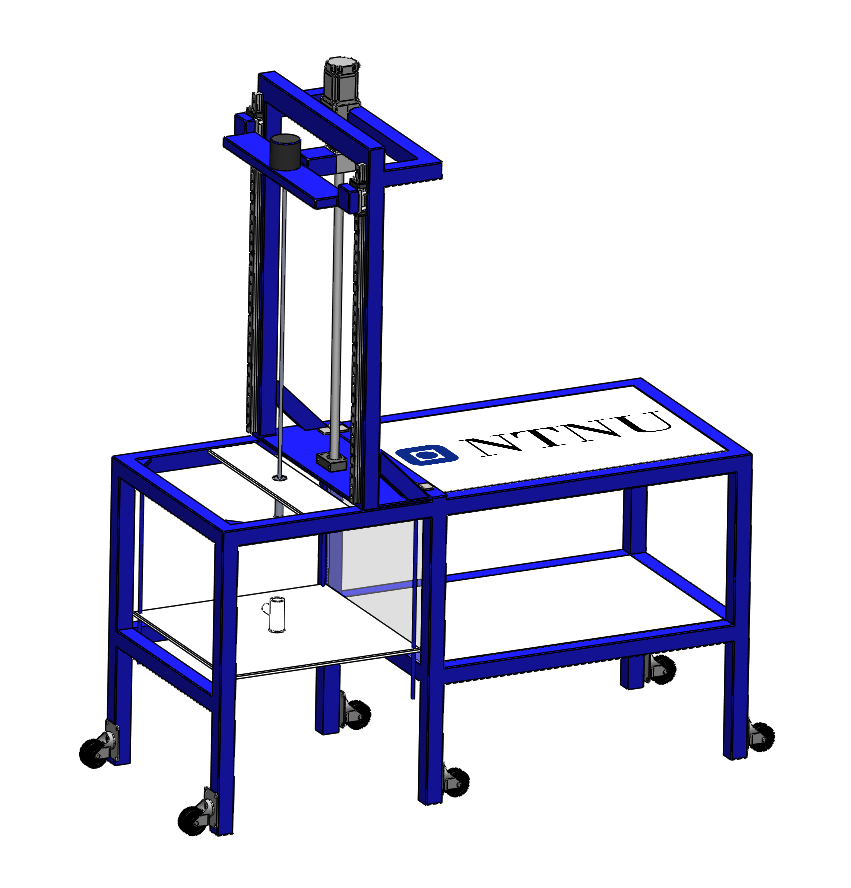
\includegraphics[width=0.5\textwidth]{figures/FrontPage.PNG}
%\caption{rig}
\label{fig:rig}
\end{figure}


% \vspace{2cm}
% \begin{figure}[h]
% \centering
% \includegraphics[width = 12cm]{figures/Forside_gambrel_real.PNG}
% \end{figure} 
\vfill
\end{titlepage}

\clearpage

\pagenumbering{Roman}

\section*{Abstract}
SPE's sub-committee DSATS (Drilling System Automation Technical Section) has organized a student competition in an effort to accelerate the uptake of automation in the drilling industry. The competition is called Drillbotics \texttrademark and this report is NTNU's contribution. 

The drill pipe and the drill bit will be provided by DSATS and the dimensions have been provided in the guidelines. The drill pipe is made of aluminium, has a length of 914 mm, and, an outer diameter of 9.53 mm and an inner diameter of 7.75 mm. The bit is a polycrystalline diamond compact (PDC) bit and has an outer diameter of 28.6 mm. The properties of the formation rock are unknown, but the dimensions are stated and are 30cmx30cmx60cm. The total maximum length of the stabilizers is limited to 90 mm. The total power consumption is limited to 25 hp and the weight on bit (WOB) is unlimited.

The main objective of the competition is to design a fully automated drilling rig that can autonomously drill a vertical well as quickly as possible while maintaining rig and drill string integrity. The purpose of this report is to present the team's solution to the problem and describe the rig's main design features.

The proposed rig design has been developed based on new ideas and innovative solutions, as well as current industry practices and guidelines provided by DSATS. Through research and analysis, an evaluation of the most likely drilling related problems and dysfunctions has been made and this has provided the basis for the dimensioning of the drilling machine and the architecture of the control system.

One of the main issues addressed in the report is how to ensure sufficient WOB without causing pipe failure. The idea is to solve this problem by adding a nozzle in the pipe which will increase its internal pressure and reduce the risk of failure. 

Another important design feature is how the system responds to drilling dysfunctions. Using an optimization function, the control system will use input data from downhole and surface sensors to adjust the control parameters. One of the most important measurements is downhole string vibrations. Large vibrations result in loss of energy and pipe fatigue and the optimization function will therefore seek to minimize their amplitude. In addition to this, key drilling parameters such as torque and ROP will be monitored and included in the optimization function to ensure high drilling efficiency.

\newpage

\section*{Team Bio}
Sigve

John Morten

Noralf and Steffen

Runa

Martin

Mayuran

Astrid

\newpage

\tableofcontents

\newpage

\pagenumbering{arabic}

\newpage
\section{Introduction}
\label{sec:1}
The oil and gas industry seeks new solutions to lower costs and improve safety and efficiency. In the last decades, the interest in drilling automation has grown as oil and gas prospects have become more complex and more challenging. An increased level of automation may result in a more accurate and rapid response to drilling anomalies, as well as a decrease in the need of human intervention during drilling operations.

As a response to this, SPE formed the sub-committee DSATS (Drilling System Automation Technical Section) to accelerate the uptake of automation in the drilling industry. During the last 2 years, DSATS has organized the international student competition Drillbotics \texttrademark. 

The aim of the competition has been to “design a drilling rig and related equipment to autonomously drill a vertical well as quickly as possible while maintaining borehole quality and integrity of the drilling rig and drill string” (ref*). The only manual intervention allowed is to press a button to start the drilling operation. This design report is NTNU’s contribution to the competition.

Several rules are presented in the guidelines and they form the basis and limitations of the design. The most important limitations are related to the pipe, drill string design, mobility of the rig, and, downhole and surface measurements of drilling parameters. These limitations have been taken into consideration when designing the drilling rig. In addition to this, the evaluation committee has listed a set of different grading criteria. This has included safety, mobility of rig, design considerations and lessons learned, mechanical design and functionality/versatility, simulation/model/algorithm and control scheme. 

Another important factor is the rig and material cost. This has been limited to US\$ 10,000 and must be covered through funding. Equipment can be provided by the university or by companies that are interested in supporting the project. The cost of this is not included in the budget. The source of funding for this project is mainly the institute, but maybe also industry. 

The main mechanical design features of the rig have been developed based on the limitations of the system. Through analysis and previous experiences, it has been clear that the weakness of the drill pipe would present the largest issue. An expected result of this is large and destructive pipe vibrations. 

The rig has been designed to minimize the magnitude of these vibrations and thus reduce their impact on the equipment. The proposed solution is to add an adjustable plate that will be positioned over the formation block and provide a point of stabilization to the drill pipe during operation. An additional point of support will be provided through a fixed plate positioned under the top drive, simulating a drill deck.

Vibrations will also be taken into consideration through the design of the drill string. To minimize the amplitude of the vibrations the total length of the drill string will be kept as short as possible and the bottom hole assembly will include a welded spiral blade stabilizer.
 
Another issue related to the weakness of the drill pipe is that it limits the amount of weight that can be applied at the top of the string. If too much weight is applied, the pipe enters a state of compression and if it reaches a critical load, it can buckle and fail. The weight added at the top is directly related to the force exerted by the formation on the bit, commonly referred to as weight on bit (WOB), which means that insufficient weight at the top reduces the ability to drill efficiently through the formation. As one of the main goals of the competition is to drill as fast as possible, it is crucial to optimize the WOB while staying within the critical load criteria.

To optimize the WOB, it has been proposed to add a nozzle in the pipe to increase its internal pressure. This will in turn lead to an increase in tension which counteracts the WOB. The increase in internal pressure is limited by the burst pressure of the pipe.

In addition to a good mechanical rig design, it has been of great importance to develop a control network and algorithms that can ensure that the automated drilling operation is safe and efficient.

One of the objectives has been to create an algorithm that continuously tries to determine the optimal control parameters. The control parameters are in this case the amount of weight applied on the string (WOB), the rotational speed of the string (RPM) and the flow rate of the drilling mud. Adjusting these parameters causes a change in other drilling parameters that will be monitored by downhole and surface sensors.

The optimal combination of control parameters will be estimated by implementing an optimization function. The goal of the function is to increase the speed of drilling, but more importantly, respond to drilling dysfunctions and ensure that all drilling parameters are within a pre-defined safe range to ensure a vertical borehole and maintain the integrity of the drilling rig and the drill string. 

The optimization function will seek to minimize the amplitude of the vibrations and maximize the speed of drilling by adjusting control parameters and monitoring the response of key drilling parameters. The response time of the sensors, data aggregation system and algorithm must be fast in order to ensure real-time data handling. Calibrating the sensors will also be an important factor in maintaining a high quality control system. 

\newpage
\section{Safety}
\label{sec:2}
One of the main concerns during any operation, regardless of its scale or scope, is the health and safety of the personnel. By automating the drilling process, the need for manual intervention is reduced and this in turn results in a safer 
drilling operation. The improved safety, as well as the increased efficiency and reduced costs, are some of the main advantages of automating drilling processes.

Although manual intervention is not required for a normal drilling operation, the construction, installation and transportation of the rig require physical labor which increases the risk of hazardous situations. Any unplanned 
incidents requiring manual intervention during drilling must also be considered.

Most accidents on a full-scale platform occur on the drill floor, especially during pipe handling \cite{drillcon}. Due to the scale of the rigs in this competition, this will not be an issue, so it is important to bear in mind that if this design were to be used for a full-scale operation, the safety hazards would be of a different nature.

The main safety hazards during the construction and operation of this drilling rig have been identified and safety 
precautions have been proposed in the sections below.

\subsection{Safety Hazards during Construction}
\subsubsection{Rig Construction}

During the period of construction of the rig, the hazardous situations will mostly be mechanical. The handling of equipment, material and debris will be the main concern.

To minimize the risk of any accidents occurring, safety glasses and protective footwear should be worn. Hearing protection, gloves and coveralls may also be required during construction activity. The construction area will be kept off limits to people not involved in the project.

As mentioned in the introduction, because of the small scale of the rig and the light weight of the equipment, the risk of any severe damage occurring is very small.


\subsubsection{Electrical Practices}
Safety related work practices will be used during the construction phase to prevent injuries resulting from electrical shock. No power will be supplied while connecting wires and components. All electrical connections will be secured and wiring will be insulated. Qualified personnel will be responsible for the high voltage setup in to the rig, while low voltage will be arranged by team members \cite{mtu}.

\subsection{Storage and Maintenance}
Any chemicals used will be documented. Disposal of waste must be controlled and done as stated in regulations.


\subsection{Safety During Transportation}
The rig is designed to ensure safe transportation. The derrick will be folded down to increase maneuverability and stability by lowering the center of mass. Jack-up casters are put on each leg to avoid heavy lifts for personnel and ensure easy rolling movement of the rig. 


\subsection{Safety Hazards During Operation}
\subsubsection{Unloading and Handling of Rock Sample}
The rig is designed to operate with the rock sample placed on the ground. This means that the rig will be maneuvered in place, instead of moving the rock sample around. No heavy lifting during rig up/down and operation will be needed, thereby reducing the risk of personnel injury and equipment damage.  


\subsubsection{Electrical System}
The water and the electrical system will be separated to avoid shorting and electrical hazards. All electrical components will be stored inside waterproof housing. Electrical cables will follow the motion of the carriage and will be exposed to wear because of bending and twisting. The state of the cables will continuously be monitored and changed if necessary. 


\subsubsection{Safety Factors and Dimensioning}
Safety factors will be applied to all calculations regarding failure of equipment. The motors and the pump will be dimensioned to fit the required criteria, such as operating RPM intervals and pump rate. The selected pump for the system has a higher pressure rating than required during the operation, a safety valve will therefore be included to ensure that the pressure does not exceed the critical values of the system. 


\subsubsection{Control System}
The control system and algorithm obtained will ensure the system is operating within safe intervals for weight on bit, torque, pressures and rotational speeds. These values have been implemented to avoid failure due to buckling, twist-off, burst and vibrations. Safety has the highest priority in the control system in which operating parameters will continuously be checked to be within safe range. If the parameters are outside the safety interval, the system will respond accordingly. Depending on how critical the values are, the algorithm will reduce RPM and WOB, lift the bit of bottom or shut down. 


\subsubsection{Emergency Shutdown of System}
Although the drilling process is fully automated, uncontrolled situations can occur. A manual stop button will cut the power supply to the motors and pump in case of emergency. The motion of the ball screw will stop immediately and keep the carriage in place. 

\newpage
\section{Mechanical Design and Functionality}
\label{sec:3}
\numberwithin{equation}{section}
\numberwithin{figure}{section}
\numberwithin{table}{section}

The rig design is based on the design criteria given in the competition guidelines. Mobility, functionality, versatility, stability, and safety have been the main concerns while designing the rig. The focus has been on having a hoisting and rotary system with high precision and functionality to ensure an efficient drilling operation. Using equipment that is already available in the university workshop has been a key concern to make the project as cost efficient as possible.

\subsection{Rig Structure}
Steel has been chosen as construction material for the main structure of the rig to ensure rigidity and stability. It also has the benefit of being cost efficient and easily accessible. Aluminum profiles were also considered, but were not chosen due to its high cost. The weight of the rig construction will be 100kg, using steel as construction material.    

The height of the drilling rig was estimated based on the rock sample height (0.60 m) and the total length of the assembled drill string. Since no making or breaking of connections will be done, the length of the drill string will be customized to drill through the block in one go. The total length of the drill string accommodates for a full length of drill pipe (0.914 m), bottom hole assembly and bit. Refer to figure (\ref{fig:SideViewUp}), (\ref{fig:SideViewUpDim}) and (\ref{fig:FrontView}) for illustration and dimensions of the rig structure. 
\begin{figure} [H]
\centering
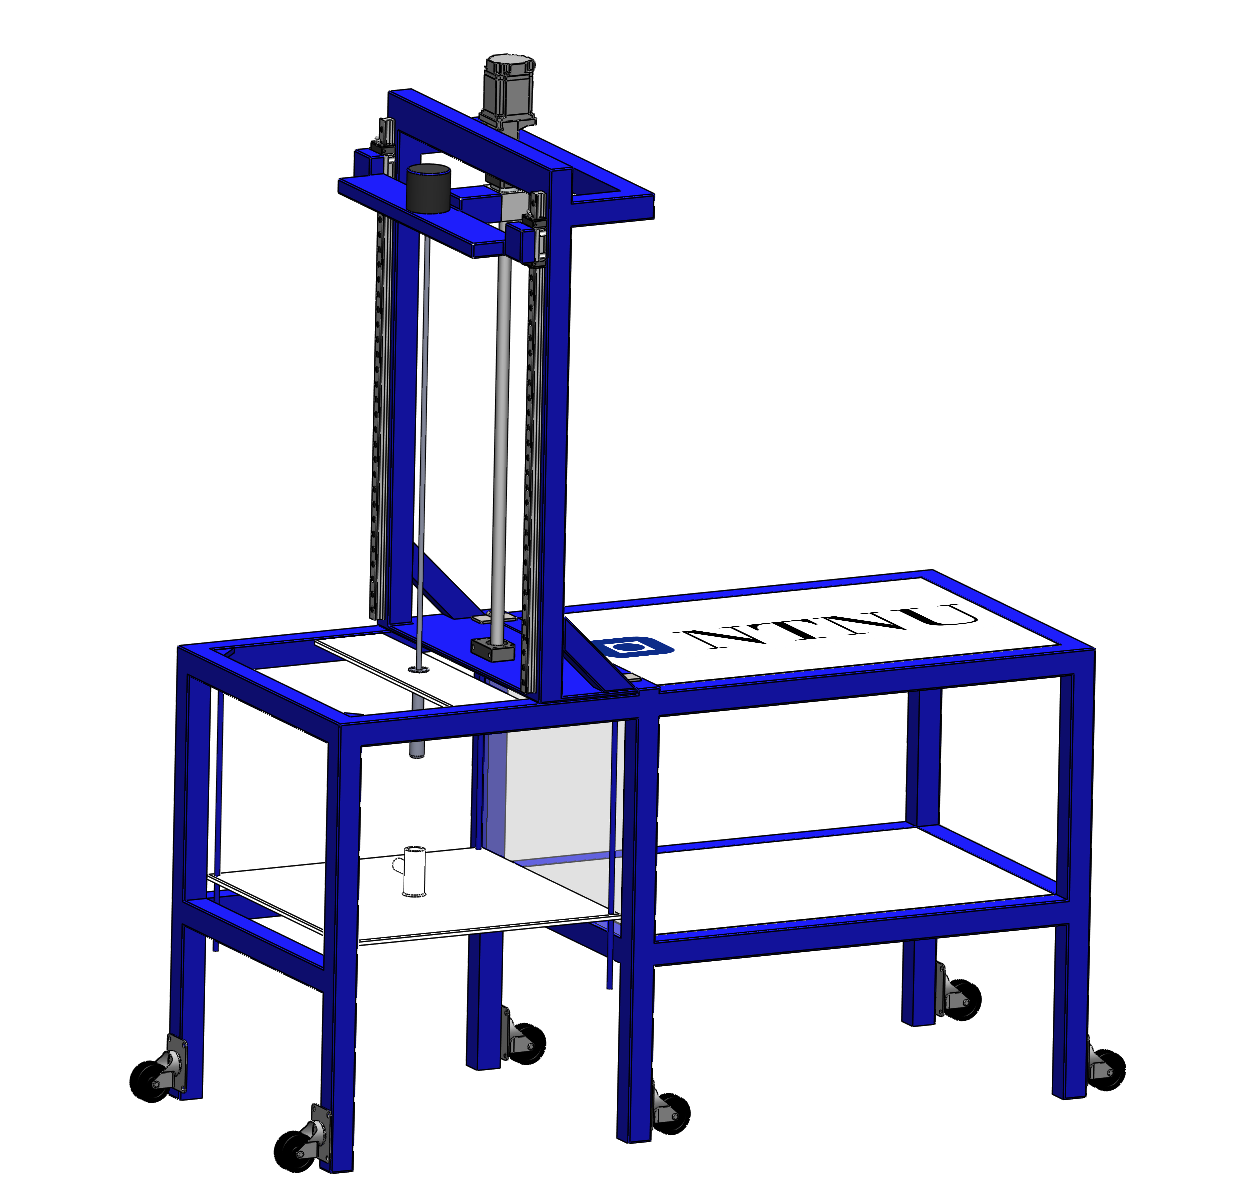
\includegraphics[width=0.6\textwidth]{figures/SideViewUp.PNG}
\caption{Illustration of the rig rig in upright position}
\label{fig:SideViewUp}
\end{figure}

\begin{figure} [H]
\centering
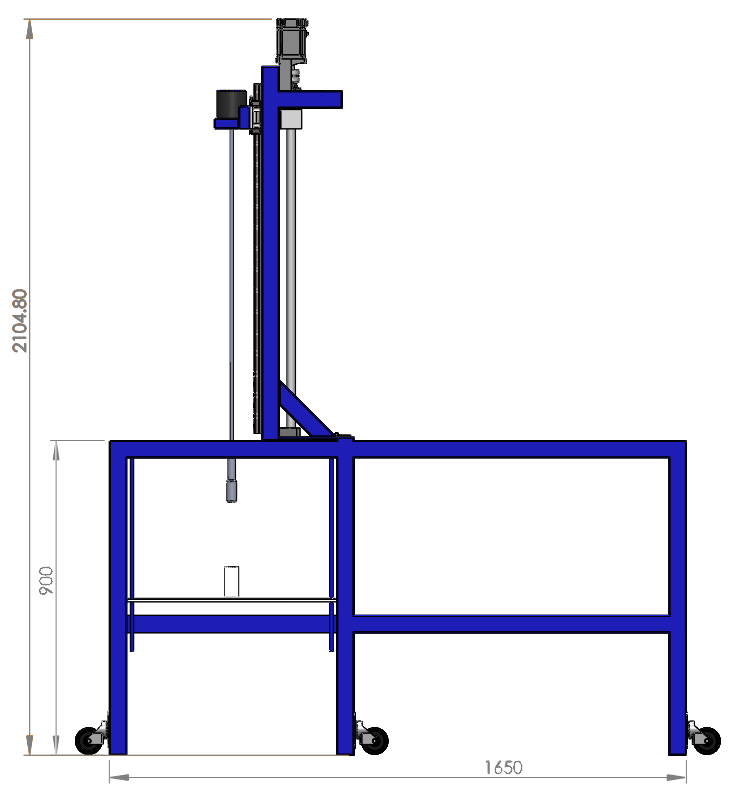
\includegraphics[width=0.6\textwidth]{figures/Sidedimensions.PNG}
\caption{Side view of the rig in upright position (dimensions in mm)}
\label{fig:SideViewUpDim}
\end{figure}


\begin{figure} [H]
\centering
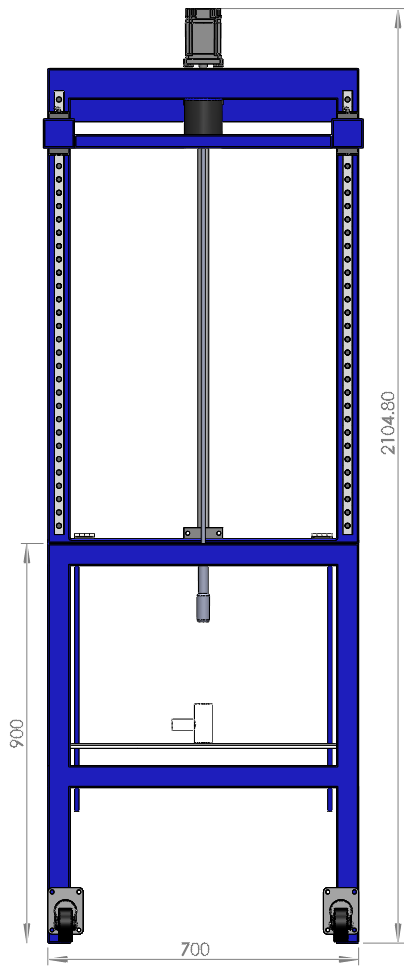
\includegraphics[width=0.3\textwidth]{figures/FrontDimensions.PNG}
\caption{Front view of the rig in upright position (dimensions in mm)}
\label{fig:FrontView}
\end{figure}


Because versatility has been important when designing the rig, the height and width of the structure were chosen to allow for a formation height up 70 cm and width up to 60 cm.

An adjustable steel plate with a thickness of 10 mm, guided by rails, will be lowered down to the formation top. The plate will, together with clamps, keep the formation at bay when drilling. A steel cylinder with a length of 80 mm and an inner diameter of 30 mm will be welded to the plate. It will be centered on the plate and work as a guiding shoe for the bit. Because the steel cylinder imitates the function of a riser, it will be referred to as a riser in the text.

\begin{figure} [H]
\centering
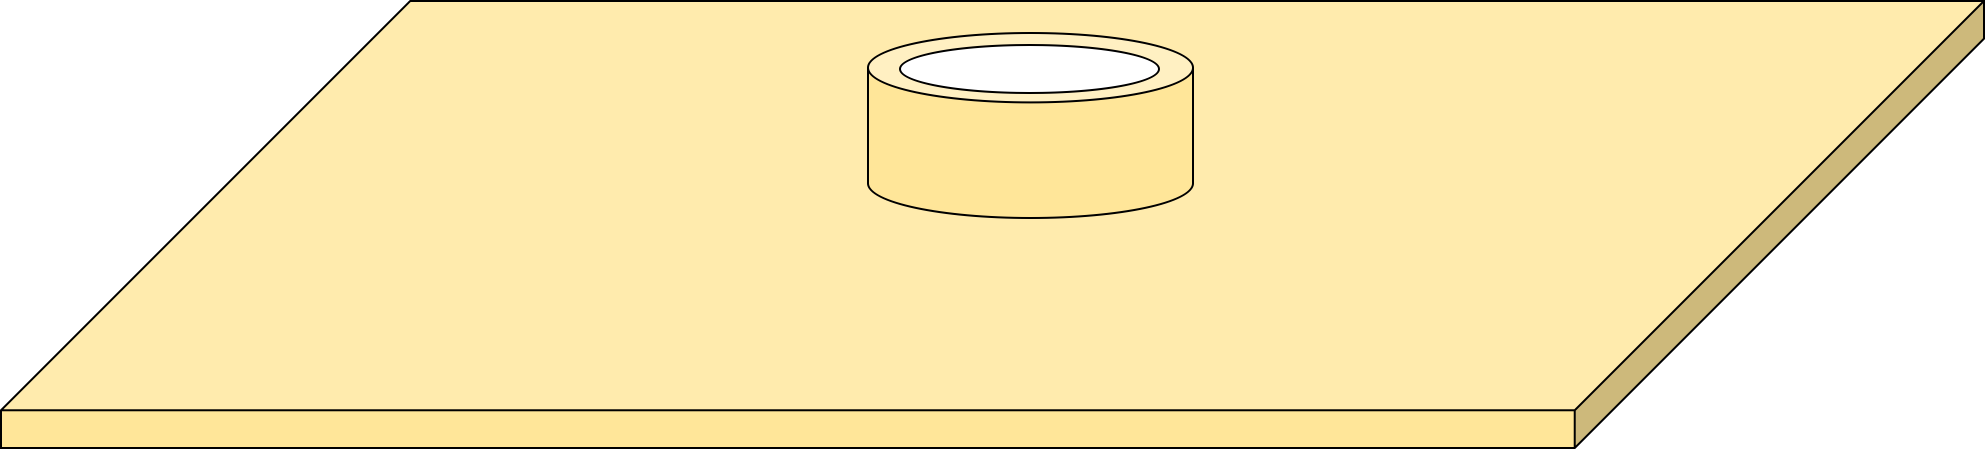
\includegraphics[width=0.6\textwidth]{figures/riser.png}
\caption{Illustration of steel plate and attached riser}
\label{fig:riser}
\end{figure}

A second cylinder with a length of 30 mm and an inner diameter of 10 mm will sit on the top of the BHA. It will consist of two parts: a hanger and a body. The hanger, of length 10 mm, will have an outer diameter larger than the outer diameter of the riser, and the body, of length 20 mm, will have an outer diameter smaller than the inner diameter of the riser. This will make it possible to land the cylinder on the riser.

\begin{figure} [H]
\centering
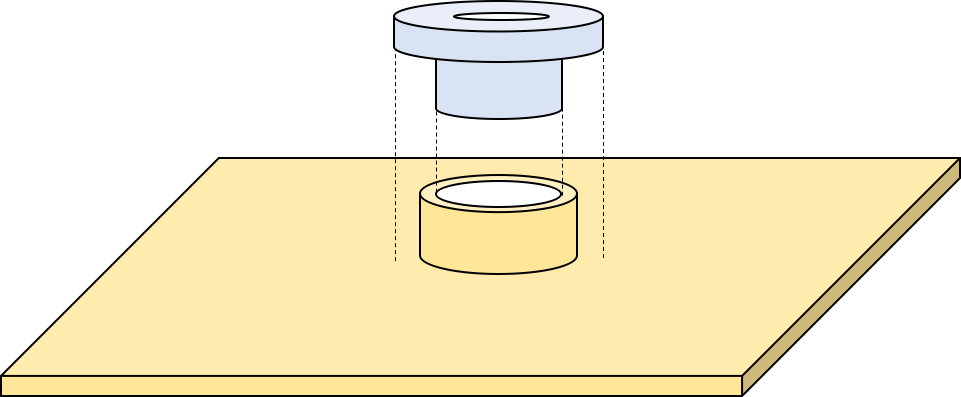
\includegraphics[width=0.6\textwidth]{figures/surfacestabilizer.png}
\caption{Illustration of steel plate, riser and surface stabilizer}
\label{fig:surfacestabilizer}
\end{figure}

As the drill string moves downwards, the cylinder will be guided into the riser and the hanger will make sure it stays inside the riser. This will provide stability for the drill string once the BHA and bit have entered the formation, and will therefore be referred to as a surface stabilizer. The combination of the riser and the surface stabilizer will provide stability during the entire drilling operation. See figure (\ref{fig:conductor}).
\begin{figure} [H]
\centering
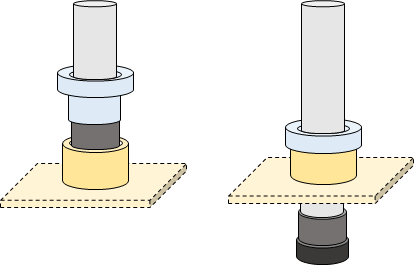
\includegraphics[width=0.6\textwidth]{figures/ConductorStab.png}
\caption{Illustration of riser and surface stabilizer}
\label{fig:conductor}
\end{figure}


A kelly bushing, in the form of a roller bearing, will be attached to the drill deck floor and serve as a stabilizing element to prevent excessive lateral vibrations and also imitate the actual drilling operation as much as possible. The inner diameter of the roller bearing will be slightly larger than the outer diameter of the drill pipe. The pipe will be guided through the roller bearing before BHA and bit is attached to the string. See figure (\ref{fig:Roller}). This roller bearing can easily be removed if the judges disallow it. 

\begin{figure} [H]
\centering
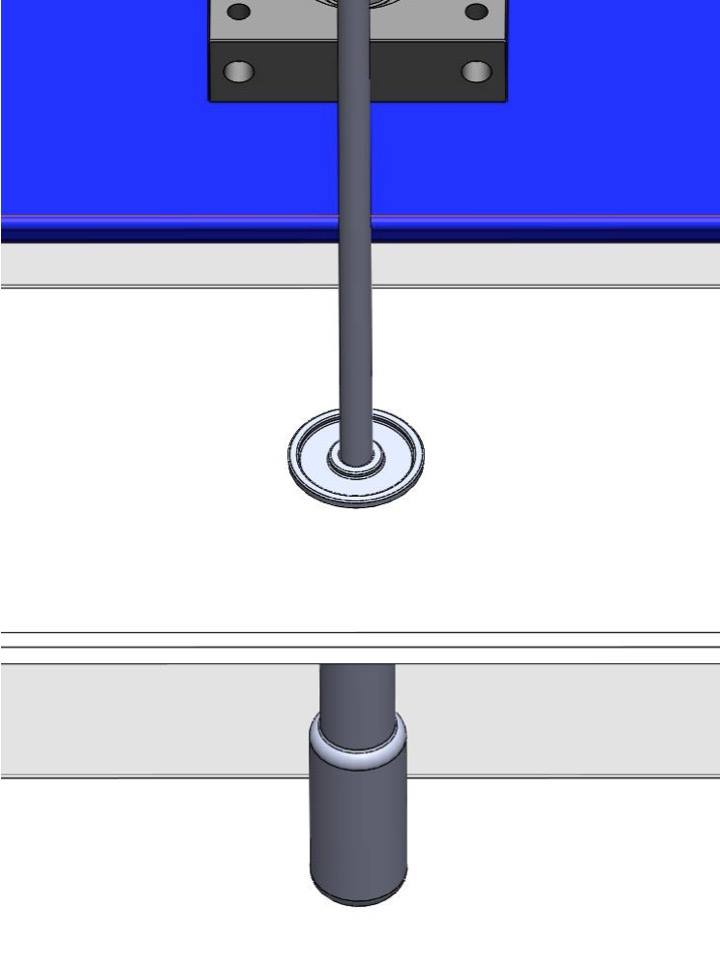
\includegraphics[width=0.5\textwidth]{figures/Roller.jpg}
\caption{Illustration of drill string running through roller bearing}
\label{fig:Roller}
\end{figure}

\subsection{Mobility of Rig}
The drilling rig is designed to easily be moved around, as well as to ensure quick rig up and rig down. Jack up casters are used on each leg to allow for mobility so that the rig can effortlessly be operated by one person. The casters will also make it possible to put the structure down on its steel legs to ensure stability when operating. The derrick is mounted to the rest of the structure by hinges and bolts, and can be folded down for a steady and safe transport. The structure is designed to be able to pass through a standard doorway, with a folded down height and width of 1.266 m and 0.7 m, respectively. Figure (\ref{fig:SideViewDown}) and (\ref{fig:SideViewDownDim}) illustrate the folded position of the rig with dimensions. 

\begin{figure} [H]
\centering
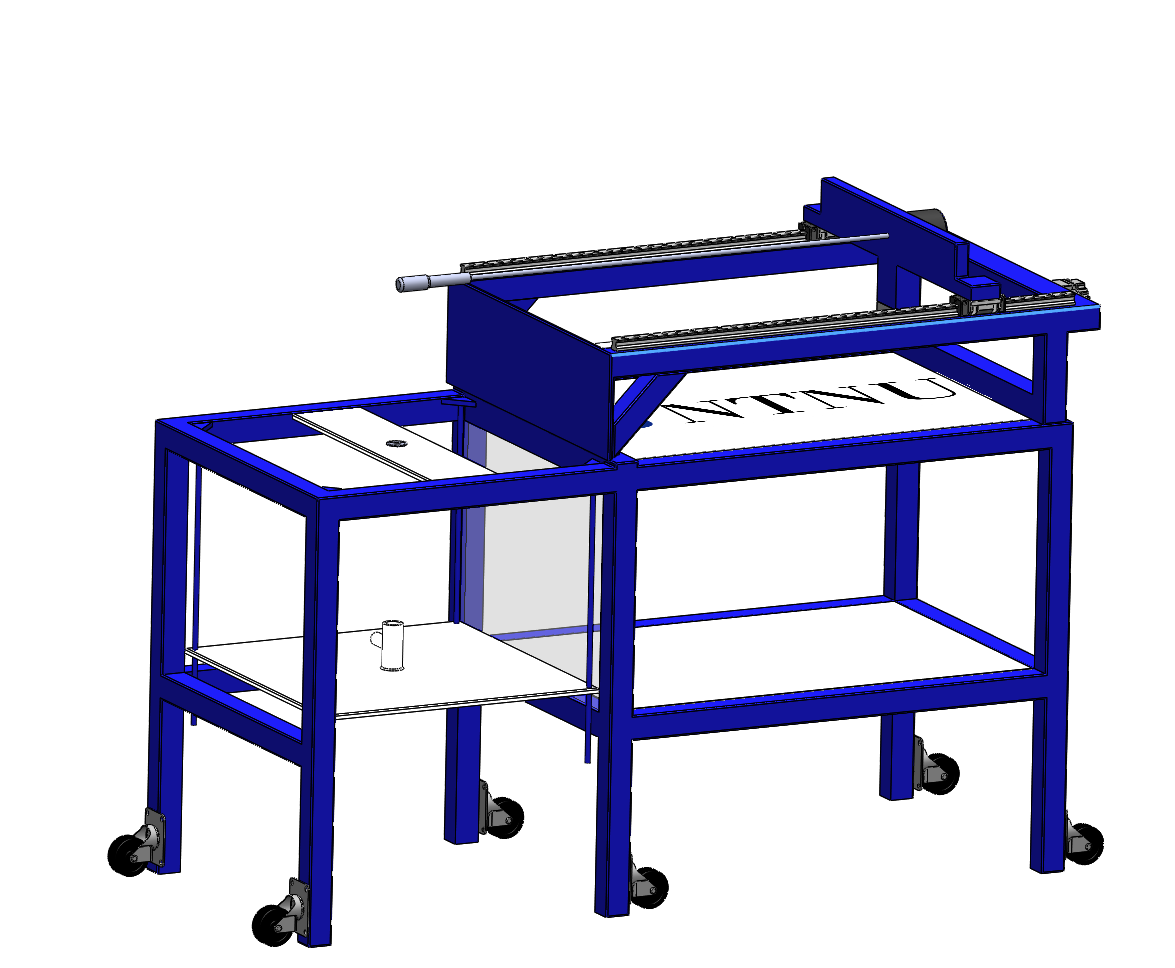
\includegraphics[width=0.7\textwidth]{figures/SideViewDown.PNG}
\caption{Illustration of the rig in folded position}
\label{fig:SideViewDown}
\end{figure}


\begin{figure} [H]
\centering
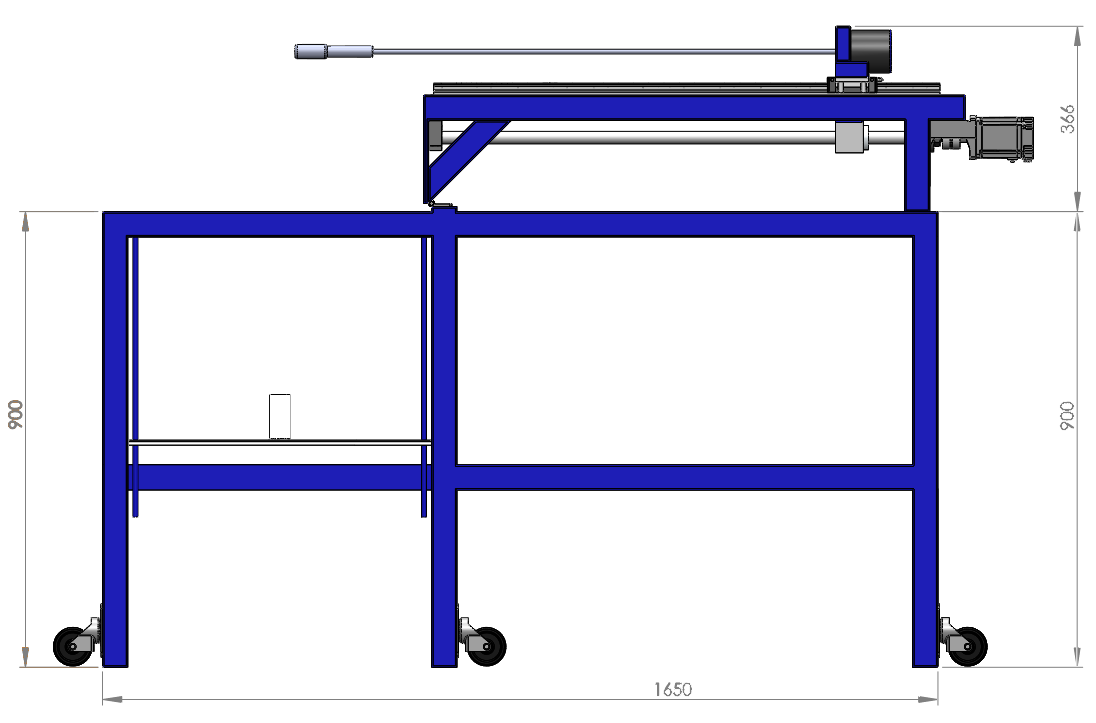
\includegraphics[width=0.7\textwidth]{figures/SideDimensionDown.PNG}
\caption{Side view of the rig in folded position (dimensions in mm)}
\label{fig:SideViewDownDim}
\end{figure}




\subsection{Hoisting System}
The hoisting system provides vertical movement of the travelling block assembly to perform the drilling operation. A traditional hoisting system with drawworks was considered, but found to be inapplicable because of its complexity and lack of precision. Unlike the traditional situation, this hoisting system needs to be able to push down the string to apply weight on bit. Rack and pinion drive was weighed against ball screw drive, where the ball screw was selected due to a higher accuracy and step resolution. 

\begin{figure} [H]
\centering
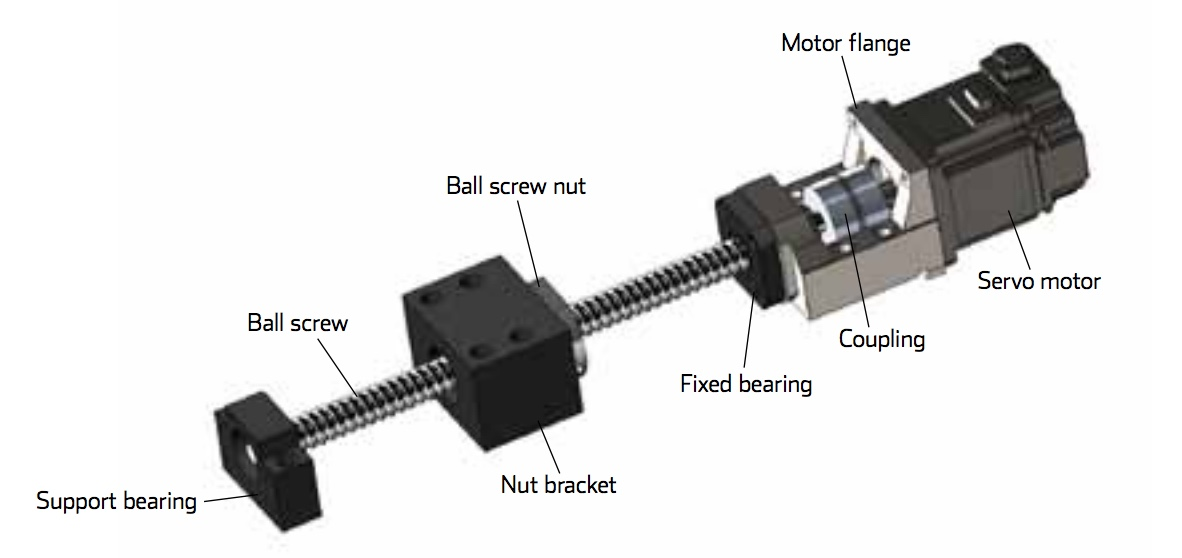
\includegraphics[width=0.7\textwidth]{figures/CompleteBS.jpeg}
\caption{Illustration of the complete ball screw package (MBA20-E-Comp) that will be used for the hoisting system \cite{aluflex}}
\label{fig:ballscrew}
\end{figure}

A 24 V DC-motor will drive the ball screw which converts rotational energy to linear motion. Because of the mechanical advantage of the ball screw, this motor will not need a high torque-output, but rather a high RPM. The power calculations for the motor will be performed in section 4.3.

A linear roller guide system will be combined with the ball screw to provide stable vertical motion and eliminate horizontal movement.

\begin{figure} [H]
\centering
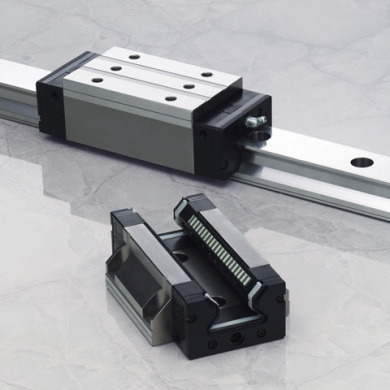
\includegraphics[width=0.5\textwidth]{figures/rollerguide.jpg}
\caption{Illustration of linear roller guide for hoisting system \cite{pic_rail}}
\label{fig:rollerguide}
\end{figure}


The linear roller guide is a low friction system which will ensure accurate WOB-measurements. It will also provide stability and high rigidity to the structure. The lead of the ball screw, together with motor selection, makes it possible to decide the hoisting speed and accuracy. An accurate hoisting system, with a low-lead ball screw, facilitates small incremented and precise weight on bit changes. 



\subsection{Rotary System}
The main function of the rotary system is to provide torque to the bit through the drill string. Both rotary table and top drive system have been considered, where the top drive system was chosen as the best solution. Even though the rotary table system would have made it easier to design the circulation system, the top drive system contains less components and provides higher power efficiency since the motor is directly connected to drill pipe. 

The top drive system will consist of a 24 V DC-engine, and the required motor power will be calculated in section 3.5. A swivel will also be included to implement the circulation system. 



\subsection{Drill String Design}
The drill string consists of a drill pipe and a BHA. The combined length of the drill string will be kept as short as possible to mitigate vibrations. It is stated in the competition guidelines that at least one length of drill pipe (91.4 cm) must be used. The BHA will be optimized to fit both the sensors and stabilizer, and will therefore have a length of 80 mm. Since the surface stabilizer has a length of 30 mm, the stabilizer in the BHA will be limited to a length of 60 mm to fulfill the requirements in the guidelines. The drill bit will have a maximum length of 64 mm.    

One of the main judging criteria is the verticality of the borehole. Stabilizers will be used to control the hole deviation and counteract vibrations. Several types of stabilizers have been considered, shown in tabel (\ref{tab:evastab}), where the welded stabilizers were chosen as the best suited solution due to their simplicity. 


\begin{table} [H]
    \centering
    \caption{Evaluation of Stabilizers}
    \begin{tabular}{p{2cm}|p{3cm}|p{3cm}|p{3cm}}
        Type & Description & Pros & Cons \\ \hline \hline
        Integral blade & Blades are an integral part of the tool body & No risk of leaving components into wellbore & Difficult to machine, expensive \\ \hline
        Welded blade & Blades are welded on to the tool body & Easy to make, cheap & Weak points in welding  \\ \hline
        Sleeve type & Replaceable sleeve mounted onto the tool body & Replaceable & Needs threading  \\ \hline
        Non-rotating & Rubber sleeve – remains stationary while the string rotates & Less wear on the blades, good for hard formations & Difficult to make, expensive  \\
    \end{tabular}
    \label{tab:evastab}
\end{table}


The main body of the BHA will have an outer diameter of 22.9 mm. To minimize frictional forces, the stabilizer blades will have an outer diameter of 28 mm, which is slightly smaller than the diameter of the wellbore being drilled. Spiral blades will be used, and the distance between the blades will provide enough space to transport cuttings and avoid pressure build-up in the wellbore. An illustration of the stabilizer is shown in figure (\ref{fig:stabilizer})

\begin{figure} [H]
\centering
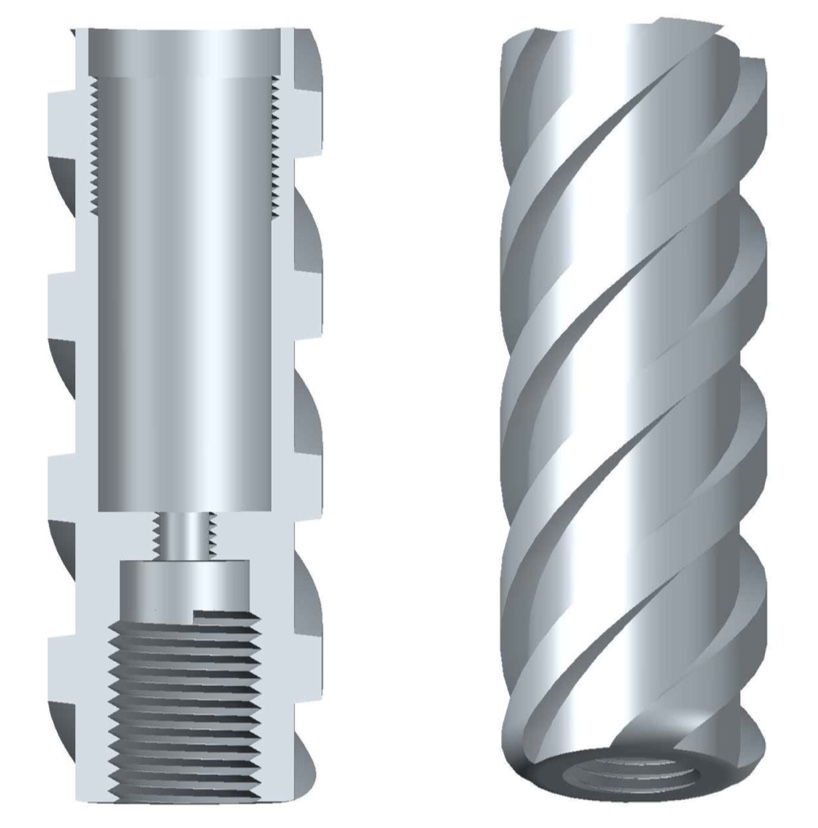
\includegraphics[width=0.5\textwidth]{figures/Stabilizer.jpeg}
\caption{Illustration of the stabilizer, showing a side cut on the left hand side}
\label{fig:stabilizer}
\end{figure}



Hydraulic connections will be used as tool joints between the BHA and the pipe as well as between the pipe and the swivel. The internal pressure in the drill string may exceed 40 bar to increase the internal stiffness in the pipe. Hydraulic connections have been chosen because of this high pressure felt by the drill string during operation. 

\newpage
\section{Power Consumption Estimation}
\label{sec:4}
The power system consists of a top drive motor, a hoisting motor, a fluid pump and a computer for the control system. As stated in the guidelines, the total power consumption cannot exceed 18.64 kW. This means that the fatigue of the system components will be the limiting factor rather than the electric power available. However, the operation should be as energy efficient as possible and the expected electrical loads will therefore be calculated.   

\numberwithin{equation}{section}
\numberwithin{figure}{section}
\numberwithin{table}{section}


\subsection{Top Drive Motor}
The top drive motor is dimensioned from the pipe torque limit as the drill pipe is the weakest element in the system. The torque limit for the drill pipe was calculated using the triaxial failure criterion showed in equation (\ref{eq:triaxialfc}). The critical point was set to be at the top of the drill pipe, where the largest axial force and internal pressure are felt. 


\begin{equation}
\centering
   (\sigma_\theta - \sigma_z)^2 + (\sigma_r - \sigma_\theta)^2 + (\sigma_z - \sigma_r)^2 = 2\sigma_{ys}^2
\label{eq:triaxialfc}
\end{equation}

$\sigma_\theta$ is the tangential stress (Pa) given by equation (\ref{eq:sigmat}), $\sigma_r$ is the radial stress (Pa) given by equation (\ref{eq:sigmar}), $\theta_z$ is the axial stress (Pa) given by equation (\ref{eq:sigmaz}), $\tau$ is the shear stress (Pa) and $\sigma_{ys}$ is the yield strength of aluminum (Pa).

\begin{equation}
\centering
   \sigma_\theta=\frac{(\frac{d_o}{2})^2+(\frac{d_i}{2})^2}{(\frac{d_o}{2})^2-(\frac{d_i}{2})^2}
\label{eq:sigmat}
\end{equation}

\begin{equation}
\centering
   \sigma_r=-P_i
\label{eq:sigmar}
\end{equation}

\begin{equation}
\centering
   \sigma_z=\frac{(\frac{d_i}{2})^2 P_i}{(\frac{d_o}{2})^2-(\frac{d_i}{2})^2}
\label{eq:sigmaz}
\end{equation}

$P_i$ is the internal pressure in the pipe (Pa), $d_o$ is the outer diameter of the pipe (m) and $d_i$ is the inner diameter of the pipe (m). 

The torque limit for the pipe was then calculated using equation (\ref{eq:tcrit}).

\begin{equation}
\centering
   T_{crit} \approx \tau_{crit} \frac{\pi}{4} (d_o^2-d_i^2)\frac{d_o+d_i}{4}
\label{eq:tcrit}
\end{equation}

$T_{crit}$ is the critical torque limit (Nm) and $\tau_{crit}$ is the critical shear stress (Pa).

The yield strength of the aluminum pipe has been assumed to be 96.55 MPa, the outer diameter of the pipe is 9.53 mm, the inner diameter of the pipe is 7.75 mm and the internal pressure is 5.26 MPa. The critical shear stress of the pipe has been calculated to be 55.66 MPa. This gave a critical torque limit of 5.80 Nm. 

Shaft power for the top drive motor is given by equation (\ref{eq:shaftpower}) \cite{bourg}.

\begin{equation}
\centering
   P_{TD}=\omega T \cdot \frac{1}{\varepsilon}
\label{eq:shaftpower}
\end{equation}

$P_{TD}$ is the shaft power for the top drive motor (W), $\omega$ is the angular velocity of the shaft (rad/sec) given by equation (\ref{eq:omega}), T is torque (Nm) and $\varepsilon$ is the efficiency factor (dimensionless).

\begin{equation}
\centering
   \omega=\frac{2\pi N}{60}
\label{eq:omega}
\end{equation}

N is revolutions per minute (RPM). 

Since this system is small scale compared to a real drilling rig, and has a very unconventional bit size, it is hard to give a good estimate of the RPM interval limits. To give a rough estimate, a 1.125” bit would have 2000 RPM to get the same tangential speed as a 12.25” bit with an upper limit of 300 RPM. Critical RPM values for the system are to be avoided to reduce the impact of large vibrations. The analysis of critical RPM will be done in section 6.1. 

Using the critical torque value of 5.80 Nm, an RPM of 2000 and an efficiency factor of 0.9, the power consumption of the top drive motor was calculated to be 1350 W. This is not a fixed value and RPM will be adjusted according to the critical values for the system.

\subsection{Hoisting Motor}
The hoisting motor power was calculated in the same way as for the top drive motor, using equation (\ref{eq:shaftpower}). Torque was estimated using equation (\ref{eq:torquealu}) \cite{aluflex}.

\begin{equation}
\centering
   T =\frac{F \cdot l}{2\pi \cdot \varepsilon_{BS}}
\label{eq:torquealu}
\end{equation}

F is the force acting on the ball screw (N) and l is the lead of the ball screw (m). The total force acting on the ball screw, from weight of drill string, stiffening force, top drive motor and carriage, was estimated to be 491 N. To ensure precision while drilling, the lead of the ball screw was chosen to be 5 mm, which is the lowest lead value available from Aluflex. The efficiency factor for the ball screw was set as 0.90 \cite{aluflex}. Torque was then estimated to be 0.43 Nm.  

For calibration purposes, the carriage should be able to move from top to bottom of the guide system within 10 seconds, which results in an RPM of 1440. The efficiency factor for the hoisting motor was set as 0.9, and the motor power required was calculated to be 73 W.  

\subsection{Fluid Pump}
The fluid pump will supply power to the circulation system to ensure proper hole cleaning and to provide geometric stiffness by increasing the internal pressure of the drill string.

The power of the pump was calculated using equation (\ref{eq:pumppower}).

\begin{equation}
\centering
   P_{Pump}=pQ \cdot \frac{1}{\varepsilon}
\label{eq:pumppower}
\end{equation}

$P_{pump}$ is the power of the pump (W), $p$ is the pump pressure (Pa) and Q is the flow rate (m$^3$/s).

The factors limiting the power of the pump are the maximum pump pressure and minimum pump flow rate. The maximum pressure was estimated from the burst pressure of the pipe, as calculated in section \ref{sssec:burst}, and was found to be 5.43 MPa. The flow rate was estimated from hole cleaning requirements, as calculated in section \ref{sssec:pressureloss}, and was found to be 0.00014 m$^3$/s. The pump efficiency was set to be 0.9, which is a typical value for piston pumps \cite{pumps}. The power of the pump was then calculated to be 775 W.

\subsection{Computer}
The computer used for the control system will use approximately 70 W, which is a maximum value for a general laptop.  

\subsection{Summary}
The power distribution for the motor, pump and computer in the system is presented in table (\ref{tab:sumpower}). The total power consumption is 2.27 kW, which is only 12\% of the power consumption limit at 18.64 kW. 

\begin{table} [H]
    \centering
    \caption{System power distribution}
    \begin{tabular}{p{3cm} p{3cm}}
        Component & Power [kW] \\ \hline \hline
        Top Drive Motor  & 1350 \\ \hline
        Hoisting Motor & 73 \\ \hline
        Fluid Pump & 775 \\ \hline
        Computer & 70 \\
    \end{tabular}
    \label{tab:sumpower}
\end{table}

\newpage
\section{Drill String Compression Analysis}
\label{sec:5}

\numberwithin{equation}{section}
\numberwithin{figure}{section}
\numberwithin{table}{section}

Pipe buckling is expected to be one of the main sources of pipe failure because of the weakness of the pipe provided by DSATS \cite{dsats} and reports from previous contests. The drill string will therefore be designed to address this issue and thus limit the risk of buckling.

Buckling occurs when too much weight is applied at the top of the drill string. This puts the pipe in a state of compression where it starts bending and becomes prone to increased metal fatigue failure. Furthermore, the body of the drill pipe wears rapidly due to abrasion along the wall. The worst-case scenario is that the pipe fails because of buckling.

This phenomenon can be prevented by increasing the tension of the drill string and thus avoiding entering a state of compression. There are two ways to achieve this, one is to reduce the weight applied at the top and the other is to increase the weight in the lower part of the string.

Although reducing the weight applied by the top drive is a simple and effective solution, it will limit the amount of weight applied on the bit and thus slow down the drilling speed. Increasing the weight in the bottom hole assembly (BHA) has therefore been chosen as the best solution.

In the industry, the weight of the BHA is increased by adding drill collars and heavy-weight drill pipes. The scale of this project makes it difficult to add sufficient weight in this manner. The proposed solution is therefore to increase the tension in the pipe wall by increasing the internal pressure of the pipe. This will be achieved by adding a nozzle in the BHA which means that the increase in internal pressure will result in a force, $F_c$, acting downwards on the constriction area. 

The sum of the weight of the drill string and the force $F_c$ will define the limit of the weight applied by the top drive. This will also enable the estimation of the required diameter of constriction.

\subsection{Weight of Drill String}
    
The weight of the drill pipe may be estimated using equation (\ref{eq:masscollar}).

\begin{equation}
\centering
   m_{DP}= \frac{\pi}{4} (d_o^2-d_i^2) \rho_{al} L
\label{eq:masscollar}
\end{equation}

$m_{DP}$ is the total mass of the drill pipe (kg), $d_o is$ the outer diameter of the drill pipe (m), $d_i$ is the inner diameter of the drill pipe (m), $\rho_{al}$ is the density of the aluminum (kg/m$^3$) and L is the length of the pipe (m).

The outer diameter of the drill pipe is 9.53 mm, the inner diameter is 7.75 mm, the density of aluminum is assumed to be 2,750 kg/m$^3$, and the length is 91.4 cm. This gives a total drill pipe weight of 0.061 kg.

The weight of the BHA is 0.227 kg and the weight of the bit is 0.300 kg. These weights may be altered during phase II. The total weight of the drill string is therefore 0.588 kg.

The buoyed weight of the string can be calculated using \ref{eq:buoyedweight}.

\begin{equation}
\centering
   m_{B}= m_{DP}(1-\frac{\rho_{w}}{\rho_{al}})+(m_{BHA}+m_{bit})(1-\frac{\rho_{w}}{\rho_{steel}})
\label{eq:buoyedweight}
\end{equation}

The density of steel is assumed to be 7,750 kg/m$^3$. This results in a total buoyed weight of 0.498 kg.

\subsection{Magnitude of Force F$_c$}
Through the following calculations, the magnitude of F$_c$ will be determined to be able to estimate how much weight can be applied through the top drive without putting the drill pipe in a state of compression. An illustration of this is shown in figure \ref{fig:strekkstring}.

\begin{figure} [H]
\centering
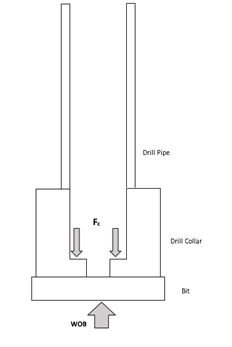
\includegraphics[width=0.5\textwidth]{figures/strekkstring.png}
\caption{Illustration of force F$_c$ counteracting the WOB and increasing the tension in the drill pipe wall}
\label{fig:strekkstring}
\end{figure}

The first step will be to calculate the burst pressure of the pipe as it is the limiting factor of the system. An estimate of the different pressure loss components in the circulation system will then make it possible to estimate the maximum value of $F_c$ and the maximum pump pressure. Finally, estimating the pressure drop over the constriction will enable the dimensioning of the constriction.

\subsubsection{Burst Pressure} \label{sssec:burst}
The limiting factor of the system is the risk of burst in the aluminum drill pipe. The increase in internal pressure inside the pipe causes an increase in differential pressure over the pipe wall which could lead to burst. Barlow’s formula, equation \ref{eq:barlow}, will be used to determine the ultimate burst pressure. 

\begin{equation}
\centering
   p_{br}=0.8 \frac{2 \sigma_{ys} t}{d_o}
\label{eq:barlow}
\end{equation}

$p_{br}$  is the maximum internal pressure the pipe can withstand (Pa), $\sigma_{ys}$ is the yield strength of aluminum (Pa), $t$ is the wall thickness of the pipe (m) and $d_o$ is the outer diameter of the pipe (m).

The yield strength of aluminum has been assumed to be 96.5 MPa, the safety factor has been chosen as 3, but may be changed during the construction phase, the thickness of the pipe wall is 0.89 mm and the outer diameter of the pipe is 9.53 mm. The burst pressure of the drill pipe has been estimated to be 5.26 MPa.

\subsubsection{Pressure Loss in Circulation System} \label{sssec:pressureloss}
The main purpose of the circulation system of this drilling rig is to provide additional internal pressure in the drill pipe to increase its geometric stiffness and reduce the risk of buckling. In addition to this, the circulation system will facilitate the removal of cuttings, cool and lubricate the drill string and bit, as well as provide well control through hydrostatic pressure. 

Fresh water was selected as drilling fluid to enable the circulation of cuttings out of the well. The use of mineral oil was considered, but due to the limited distance of transportation and the expected low pore pressure, it was concluded that fresh water was a better choice. This is a cheaper and more accessible alternative to standard drilling muds used in the industry.

\begin{figure} [H]
\centering
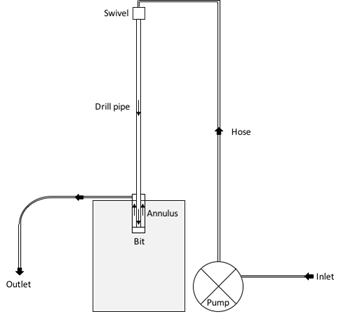
\includegraphics[width=0.5\textwidth]{figures/fluidsystem.png}
\caption{Illustration of the circulation system consisting of a mud pump, hose, swivel, drill pipe, BHA, bit nozzles and flowline.}
\label{fig:fluidsystem}
\end{figure}

A pump will be installed to both circulate the drilling fluid through the system and increase the internal pressure of the drill string. The recirculation of drilling fluid is not included in this design as it requires an advanced solid removal system. The fluid will be conducted out of the well and into a separate tank for storage. 

A density of 998.2 kg/m3 and dynamic viscosity of 0.001002 Pa·s have been used in the pressure loss calculations. This is based on the properties of water at a temperature of 20\degree C \cite{engtool}.

The fluid velocity through the different components was determined based on the minimum required flow velocity in the annulus to circulate the cuttings out of the well. It has been decided that the flow rate will be maintained constant during the drilling operation.

\paragraph{Fluid Flow Velocity}
To remove cuttings from the wellbore, the annular velocity must be greater than the cutting slip velocity. The cutting slip velocity is given by equation (\ref{eq:vsl}) which is valid for all Reynold’s numbers \cite{bourg}.

\begin{equation}
\centering
   v_{sl}= \sqrt{\frac{d_s}{f} \frac{(\rho_s-\rho_f)}{\rho_f}}
\label{eq:vsl}
\end{equation}

$d_s$ is the particle diameter (m), $\rho_s$ is the solid density (kg/m3), $\rho_f$ is the fluid density (kg/m3) and $f$ is the friction factor.

The maximum particle diameter was in this case assumed to be half the distance between the borehole wall and the outer diameter of the BHA, resulting in a particle diameter of 0.7 mm. The solid density was assumed to be 2,640 kg/m3 (based on density of granite). The friction factor $f$ can be estimated using an empirical relationship between Re, the sphere diameter and the sphericity. Because Re is dependent on the unknown slip velocity, an initial simplifying assumption must be made. To calculate the initial Reynold’s number, the slip velocity $v_sl$ will be approximated by Stokes’ relation for creeping flow around a spherical particle given by equation (\ref{eq:stoke}) \cite{bourg}.

\begin{equation}
\centering
   v_{sl}= \frac{d_s^2 (\rho_s-\rho_f)}{\mu}
\label{eq:stoke}
\end{equation}

The initial guess for the particle slip velocity is 0.42 m/s. Re can now be calculated based on the input data and the particle slip friction factor can then be estimated based on the empirical friction factor chart \cite{bourg}. Assuming a sphericity factor of 1, the friction factor is expected to be 0.6. This results in a cutting slip velocity of 0.16 m/s. Iterations were then performed until a good approximation was found. The final cutting slip velocity was found to be 0.12 m/s.
It is usually desirable to have a transport efficiency, equation (\ref{eq:va}), of 50\% or higher, the aim will therefore be to have an annulus fluid velocity of 0.25 m/s.

\begin{equation}
\centering
   v_{a}= \frac{v_{sl}}{transport efficiency}
\label{eq:va}
\end{equation}

Assuming the flow rate is constant throughout the system, the minimum flow rate delivered by the pump is then determined by multiplying the annulus velocity by the annulus cross-sectional area. The borehole diameter is approximated by the bit diameter, 28.6 mm, and the outer diameter of the pipe is 9.53 mm, this yields a cross-sectional area of 570.1 mm2. The minimum flow rate in the system is, based on these calculations, 0.00014 m3/s.
Based on the above result, the fluid velocity in the different components of the circulation system may be calculated. This constitutes the basis of the pressure loss calculations which will be conducted in the following paragraphs.

\paragraph{Pressure Loss in Hose}
The first step in the process of calculating the pressure drop through the hose is to determine the type of flow regime. This may be done by estimating Reynold’s number given by equation (\ref{eq:reynold}).

\begin{equation}
\centering
   Re= \frac{\rho v d_i}{\mu}
\label{eq:reynold}
\end{equation}

$Re$ is Reynold’s number (dimensionless), $\rho$ is the fluid density (kg/m3), $v$ is the fluid velocity (m/s), $d_i$ is the inner diameter of the pipe (m) and $\mu$ is the fluid viscosity (Pa·s). The density and the viscosity were presented in section 5.3.2.

The inner diameter of the hose is assumed to be 7.75 mm, the same as for the pipe. This is an initial estimate and will be reconsidered during phase II when equipment will be ordered.

Laminar flow is when $R_e$<2,500, transitional flow when 2,500<$R_e$<4,000 and turbulent flow when $R_e$>4,000 (Cengel, 2006). In this case, with the parameters listed above, Reynold’s number is $R_e$=23,334 which means the flow is turbulent.

In the case of turbulent flow, the friction factor must be determined using an empirical correlation. The Colebrook Equation, which is widely used in the field of fluid dynamics, was chosen as a good approximation and is given by equation (\ref{eq:friction}). It is an implicit equation and it has therefore been solved numerically using Excel.

\begin{equation}
\centering
   \frac{1}{\sqrt{f}}=-4 log (\frac{0.269\varepsilon}{d}+\frac{1.255}{Re\sqrt{f}})
\label{eq:friction}
\end{equation}

$f$ is the friction factor (dimensionless) and $\varepsilon$ is the roughness of the hose (m).

The friction factor is then used in the Fanning Equation given by equation (\ref{eq:pressuredrop}) \cite{bourg} to calculate the frictional pressure drop in the hose.

\begin{equation}
\centering
   \Delta p_f = \frac{f\rho v^2 L}{25.8 d}
\label{eq:pressuredrop}
\end{equation}

$\Delta p_f$ is the frictional pressure loss (Pa) and $L$ is the length of the hose (m). In the case of laminar flow, a simpler set of equations may be used \cite{bourg}.


The pressure drop through the hose, $\Delta p_1$, was estimated to be 190.0 kPa.

\paragraph{Pressure Loss in Swivel}
It has been assumed that the pressure loss through the swivel can be approximated by calculating the pressure loss through a regular 90\degree elbow with screwed fitting. The same method as for the pressure loss in a pipe can be used for this calculation, however, the length must be substituted by an equivalent length. Based on a pipe diameter of 7.75 mm, the equivalent length is 0.9 m \cite{engtool}.

The flow through the swivel was found to be turbulent and the total pressure drop through it, $\Delta p_2$, was estimated to be 105.4 kPa. A more accurate estimate of the pressure loss will be provided by the manufacturer of the swivel in phase II. 

\paragraph{Pressure Loss in Pipe and BHA}
The pressure loss in the drill pipe and the bottom hole assembly were calculated in the same way as the pressure loss in the hose. The inner diameter of the drill pipe is 7.75 mm and the inner diameter of the BHA is 18 mm. The length of the drill pipe is 91.4 cm m and the length of the BHA is 8 cm.

From equation (\ref{eq:reynold}) it was determined that the flow through both the pipe and the BHA is turbulent. Equation (\ref{eq:friction}) was used to determine the friction factor and, finally, equation (\ref{eq:pressuredrop}) was used to estimate the pressure drop. 

The pressure drop through the drill pipe, $\Delta p_3$, was estimated to be 107.0 kPa and the pressure drop through the BHA, $\Delta p_4$, was estimated to be 0.43 kPa.


\paragraph{Pressure Loss in Bit and Nozzle}
The pressure loss in the bit was calculated in the same way as for a pipe (equations (\ref{eq:reynold}), (\ref{eq:friction}) and (\ref{eq:pressuredrop})), but the pressure loss through the two nozzles was based on equation (\ref{eq:nozzle}).

\begin{equation}
\centering
   \Delta p_n = \frac{\rho Q^2 L}{C_d^2 A^2}
\label{eq:nozzle}
\end{equation}

$Q$ is the fluid flow rate (kg/m$^3$), $C_d$ is the discharge coefficient (dimensionless) and $A$ is the cross-sectional flow are (m$^2$). The discharge coefficient was estimated to be 0.95 and the flow area was determined assuming it consists of two nozzles with circular area, each with a diameter of 4.34 mm$^2$.

\paragraph{Pressure Loss in Annulus}
The pressure loss through the annulus was based on equations (\ref{eq:reynold}), (\ref{eq:friction}) and (\ref{eq:pressuredrop}). The value of the diameter used in these equations is an equivalent diameter calculated using equation (\ref{eq:eqdiameter}).

\begin{equation}
\centering
   d_{eq} = \sqrt{d_a^2-d_o^2}
\label{eq:eqdiameter}
\end{equation}

$d_a$ is the diameter of the annulus and $d_o$ is the outer diameter of the pipe (m).

The flow rate was estimated to be turbulent through the annulus as well and resulted in a pressure drop, $\Delta p_8$, of 0.11 kPa.

\paragraph{Summary of Pressure Loss in Circulation System}
The pressure loss trough the different components is presented in Table \ref{tab:sumpressure}. The different pressure drops have been numbered from 1-8 starting with the hose and ending with the annulus. $\Delta p_5$ is not present in the table as it represents the pressure loss over the constriction and will be calculated in the next section.

\begin{table} [H]
    \centering
    \caption{Pressure Loss in Circulation System}
    \begin{tabular}{p{3cm} p{4cm}}
        Component & Pressure Loss [kPa] \\ \hline \hline
        Hose, $\Delta p_1$  & 190.0 \\ \hline
        Swivel, $\Delta p_2$ & 105.4 \\ \hline
        Drill Pipe, $\Delta p_3$ & 107.0 \\ \hline
        BHA, $\Delta p_4$ & 0.4 \\ \hline
        Bit, $\Delta p_6$ & 1.5 \\ \hline
        Bit Nozzles, $\Delta p_7$ & 150.3 \\ \hline
        Annulus, $\Delta p_8$ & 0.1 \\ \hline
        Total, $\Delta p_{tot}$ & 553.7 \\
    \end{tabular}
    \label{tab:sumpressure}
\end{table}

The pressure drop through the different components of the circulation system will now be used to determine the force acting on the constriction.

\subsubsection{Calculation of $F_c$}
To determine the force acting on the constriction, an equation describing the pressure loss components in the system is shown in equation (\ref{eq:sumpressure}). 

\begin{equation}
\centering
   p_{pump}=\Sigma_{i=1}^{8} \Delta p_i
\label{eq:sumpressure}
\end{equation}

The parameter dimensioning the pressure at the constriction is the burst pressure of the pipe. The internal pressure of the pipe will be within this limit as long as the pressure at the top of the pipe is less than $p_{br}$. The pressure at the constriction may be determined by subtracting the pressure loss in the drill pipe and BHA from the maximum burst pressure as shown in equation (\ref{eq:pcons}).

\begin{equation}
\centering
   p_{c}=p_{br} -\Sigma_{i=3}^{4} \Delta p_i
\label{eq:pcons}
\end{equation}

From the previous section, the sum of $\Delta p_3$ and $\Delta p_4$ is 107.4 kPa and based on this the pressure at the constriction can be assumed to be 5,147.9 kPa.

To determine the magnitude of the tension force $F_c$, the area the force is acting on must be calculated. For the sake of simplicity, the area will be assumed to be the complete cross sectional area of the drill pipe. It may be calculated using equation (\ref{eq:areacons}).

\begin{equation}
\centering
   A_t = \frac{\pi}{4} d_i^2
\label{eq:areacons}
\end{equation}

The inner diameter of the drill pipe is 7.75 mm and this yields a cross-sectional area of 47.1 mm$^2$.

The hydraulic force can then be calculated by multiplying $P_c$ by $A_t$. This results in a force $F_c$ of 304.6 N, equivalent to a weight of 31.0 kg. 


\subsection{Constriction Diameter}

To calculate the diameter of the constriction, the maximum pressure drop over the constriction must be estimated. This can be calculated by subtracting the pressure loss over the bit, bit nozzles and annulus from the pressure acting on the constriction as shown in equation (\ref{eq:pdcons}).


\begin{equation}
\centering
   \Delta p_{c}=\Delta p_{br} -\Sigma_{i=5}^{8} \Delta p_i
\label{eq:pdcons}
\end{equation}

The pressure at the constriction was estimated to be 5,147.9 kPa, the pressure drop through the bit is 1.5 kPa, through the nozzles is 150.3 kPa and through the annulus is 0.1 kPa. This results in a pressure drop over the constriction equal to 4,997.1 kPa.

To dimension the size of the nozzle, equation (\ref{eq:nozzlesize}) was solved for the diameter of the nozzle using Excel.

\begin{equation}
\centering
   \Delta p_{c}=\frac{1}{2} \rho_f (1-\beta^4)(\frac{q}{C_d A_t})^2
\label{eq:nozzlesize}
\end{equation}


Where $\beta = \frac{d_n}{d_i}$.


Input data for equation (\ref{eq:nozzlesize}) can be found in table (\ref{tab:inputdata}).

\begin{table} [H]
    \centering
    \caption{Input Data for Hydraulic Force Calculations}
    \begin{tabular}{p{7cm} p{2cm}}
        Density of fluid [kg/m$^3$] & 998.2 \\ \hline
        Flowrate [m/s] & 0.25 \\ \hline
        Cd & 0.95 \\ \hline
        Pressure drop at constriction [kPa] & 4,997 \\ \hline
        Inner diameter of pipe [mm] & 7.75 \\ 
    \end{tabular}
    \label{tab:inputdata}
\end{table}

The diameter of the constriction was found to be 1.38 mm.

\subsection{Euler's Critical Load Analysis}

Even though the main goal is to keep the drill string completely in tension, it is not possible to predict how much WOB that will be required to drill through the formation and it might therefore be required to increase the WOB above the limit defined in section . To set an absolute upper limit of WOB, Euler's equation (\ref{eq:eulerbuckling}) for critical load will be used. This will enable the estimation of the maximum load the pipe can bear without experiencing lateral deflection.

\begin{equation}
\centering
   F_{cr}=\frac{\pi^2 E I}{(KL)^2}
\label{eq:eulerbuckling}
\end{equation}

where $F_{cr}$ is the critical compression load (N) on the drill pipe, $E$ is the modulus of elasticity of pipe material (Pa), $I$ is the minimum area moment of inertia of the cross section of the pipe (m$^4$) given by equation (\ref{eq:momentinertia}), $L$ is the unsupported length of the pipe (m) and $K$ is the effective length factor determined by the end conditions of the pipe given in figure (\ref{fig:endcondpipe}).

\begin{equation}
\centering
   I=\frac{\pi}{64} (d_o^4-d_i^4)
\label{eq:momentinertia}
\end{equation}

where $d_o$ and $d_i$ is the outer and inner diameter of the pipe respectively.

\begin{figure} [H]
\centering
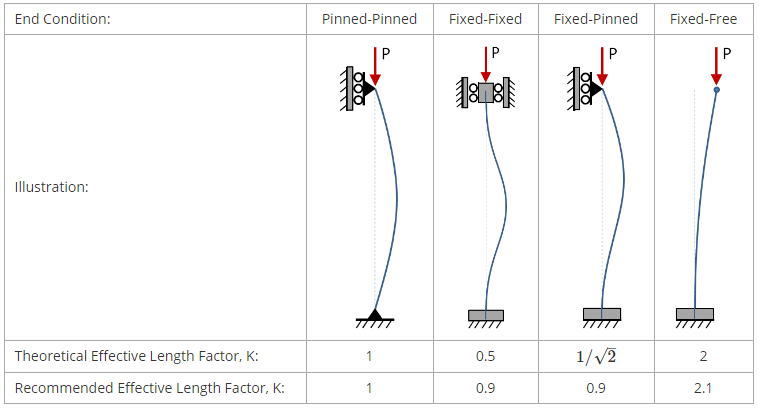
\includegraphics[width=1.0\textwidth]{figures/endcondpipe.PNG}
\caption{End conditions of pipe \cite{buckling}}
\label{fig:endcondpipe}
\end{figure}

Due to the implementation of a riser above the formation, the end conditions will be \textit{fixed-fixed}, which yields a recommended effective length factor, $K$, of 0.9.

Input data for equation (\ref{eq:eulerbuckling}) can be found in table (\ref{tab:inputdataeuler})


\begin{table} [H]
    \centering
    \caption{Input data for Euler's Critcal Load}
    \begin{tabular}{p{2cm} p{3cm}}
        E [Pa] & $6.9\cdot10^{10}$ \\ \hline
        I [m$^4$] & $2.27\cdot10^{-10}$ \\ \hline
        K & $0.9$ \\ \hline
        L [m] & $0.91$ \\ 
    \end{tabular}
    \label{tab:inputdataeuler}
\end{table}

The critical load was found to be 230.7 N, equivalent to a weight of 23.5 kg. This means that when the internal pressure is increased using the nozzle in the BHA, the pipe will enter a state of compression when the WOB passes 31.0 kg, but it will not, based on this estimation buckle until it reaches the sum of F$_c$, the drill string weight and the critical load, in this case 50 kg.

The goal will still be to avoid putting the string in compression, but if it becomes clear during phase II that a WOB of 31.0 kg is insufficient to drill efficiently, it will be considered whether a higher WOB can be used or not.

\subsection{Drill String Compression Analysis Results} \caption{ssec:comp}

\begin{table} [H]
    \centering
    \caption{Estimated values for Fc, weight of drill string and maximum WOB.}
    \begin{tabular}{p{5cm} p{2cm}}
        $F_c$ [kg] & 31.0 \\ \hline
        Weight of Drill String [kg] & 0.5 \\ \hline
        Maximum WOB [kg] & 31.5 \\ \hline
        Critical WOB [kg] & 50.0 \\ \hline
    \end{tabular}
    \label{tab:summarywob}
\end{table}

A total of 31.5 kg can be applied on the drill string through the top drive while maintaining the neutral point in the BHA when using a constriction with a flow diameter of 1.38 mm in the BHA.




\newpage
\section{Drill String and Bit Dysfunctions}
\label{sec:6}
To improve drilling performance, a closer look must be taken at the integrity of the drill string and the borehole. Drilling dysfunctions, such as vibrations and high shock loads, can cause tool failure and hole problems, which means that to maintain the integrity of the well, drilling dysfunctions should be avoided. When looking at the consequences of drilling dysfunctions, it is easy to see how much you can optimize the overall drilling operation by using a proactive approach to either prevent or reduce these destructive forces.	

Many drilling dysfunctions with critical consequences occur because of high amplitude vibrations. The causes and effects of vibrations in the drill string will therefore be reviewed. Other drilling dysfunctions such as bit balling and interfacial severity will also be reviewed, but because they are not expected to occur in this situation, they will not be the focus of this analysis. 

\numberwithin{equation}{section}
\numberwithin{figure}{section}
\numberwithin{table}{section}


\subsection{Dysfunctions resulting from Vibrations}
The causes and effects of vibrations in the drill string are of large concern. The damage caused by vibrations can be severe both in terms of safety and of drilling efficiency, and that is the main motivation behind this analysis.
Some of the damages caused by vibrations are damage to the bit cuttings and bearings, stick/slip and stuck pipe, component and connection fatigue, and wear. This can severely damage the equipment as well as reduce the drilling rate.

Vibrations are usually more violent in a vertical well because the drill string may move more freely than in deviated wells. In addition to this, using a PDC bit accentuates transverse vibrations and bit whirl because they usually have aggressive side cutters that dig into the borehole. Vibrations are therefore expected to be one of the main sources of failure and trouble in our system. 

The restrictions on WOB related to the yield strength of the pipe mean that the aim will be to maintain a high RPM to have a good ROP. This in turn means that it will be crucial to conduct a thorough vibration analysis to optimize the drilling efficiency.

The goal of this analysis is to reduce and control the vibrations. This may be done by minimizing the generation of the vibrations and/or by reducing the life of the vibrations by damping and avoiding reflections, coupling and resonance. 


\subsubsection{Background}
There are three main types of vibrations that can occur while drilling: axial, torsional and lateral. Each of these modes has a different type of destructive nature: axial vibrations can cause bit bounce, torsional mode can cause irregular downhole rotation and lateral mode can cause large shocks as the BHA impacts the borehole wall. All three vibration types can occur during rotary drilling and they can all cause significant damage.

\paragraph{Axial Vibrations}
Axial vibrations can cause bit bounce which can damage the bit and the cutters. Axial mode is not expected to have any large impact on the drilling performance and will therefore not be focused on in this analysis.

\paragraph{Torsional Vibrations}
Stick-slip is a severe form of drill string rotational oscillation and is characterized by the release and absorption of energy. Stick-slip occurs when the drill bit cutters meet the rock and a combination of the potential of the rock and friction causes the drill bit to stay stationary for a period (stick). During stick, the bit starts to absorb energy. In the release phase (slip), the bit starts to spin out of control and the energy accumulated during the stationary period is released to the rest of the drill string as turns and twists. The severity of the torsional vibrations increases as the length of the stick period increases.

\paragraph{Lateral Vibrations}
Lateral vibrations are the most destructive type of vibrations, and are, together with axial vibrations, more violent in vertical wells.  Lateral vibration shocks are caused by the interaction between the BHA and the wellbore and may cause a high-frequency, large-magnitude, bending moment which can lead the system into whirl. 

As the system is lead into whirl, the center of rotation is offset from the center of the hole, resulting in a drill string that walks around the hole as it is rotating around itself. Whirl is a result of bit vibrations and a misalignment of the drill string and BHA. It creates a fatigue damage in the drill string through bending stress cycles which may lead to failure of connections. 

To reduce the risk of damaging the drill string through vibrations, the theory behind natural frequency will be reviewed. This will create the basis of the analysis of critical RPM.

\subsubsection{Natural Frequency}
Natural frequency is the frequency at which a system tends to oscillate in the absence of any driving or damping force. When drilling through a formation, the drilling operation leads to vibrations that pass from the bit through the BHA and finally to the drill string. If the vibrations reach the same natural frequency as that of the drilling equipment, resonance is established. 
Resonance is a phenomenon that occurs when a vibrating system drives another system to oscillate with greater amplitude at a specific frequency. In this case, it may result in a higher amplitude displacement of the equipment, thus damaging it even more. 
Rotation of the bit causes vibrations that spread through the equipment (Drillstring Vibrations and Vibration modelling, 2010). It is critical to find the rotation speed, RPM, that does not create vibrations with the same frequency as the drilling equipment’s natural frequency. By avoiding the critical RPM, the lifetime of the equipment may be increased and the drilling operations will be optimized. 

\subsection{Other Drill String and Bit Dysfunctions}

\subsubsection{Bit Balling}
Bit balling is when cuttings stick to the surface of the bit and it can happen when drilling through water reactive shale or clay formations. Electrochemical and mechanical sticking are the two main mechanisms that contribute to bit balling. If poor hydraulic design is used or the mud flow is stopped, an electrostatic force may cause cuttings to stick on the surface of the bit, and once initiated, it is easier for cuttings to build up and eventually ball up the bit. \cite{schlumvib} 

Bit balling may be detected by a sudden reduction in ROP, without any significant change in other drilling parameters. The torque is usually lower than normal since the cutters are covered up by cuttings and there may also be a sudden increase in standpipe pressure because balling reduces the annular flow area which increases the pressure. \cite{bitballing}

As soon as bit balling is spotted, the best way to mitigate the problem is to reduce the WOB and increase the flow rate. By doing this, the cuttings stuck on the drill string may be washed out \cite{bitballing}.

\subsubsection{Bottom-Hole Balling}
Bottom-hole balling is the accumulation of cuttings at the bottom of the hole which can clog the hole and prevent contact between the drill bit and the rock formation. It usually occurs when the hydrostatic pressure is very high and in impermeable rock, and results in a very high MSE and a reduced ROP. The ROP is usually unresponsive to changes in WOB, so the best way to respond is to increase the pump flow rate and the RPM.

\subsubsection{Interfacial Severity}
Interfacial severity is when a harder rock, a new layer or an inclusion in the current layer, is encountered in the formation. The force on the bit is then concentrated on the part of the bit in contact with the hard rock instead of on the entire surface area of the bit. This can cause bit damage. The best response is to reduce the WOB to minimize the damage on the bit.




\newpage
\section{Algorithm/Simulation/Model}
\label{sec:7}
Automated drilling will most likely involve linking downhole and surface measurements with real-time models to improve the safety and efficiency of the drilling process. The main idea is that downhole and surface sensors will communicate measurements to a computer which in turn will display and process the data, as well as control drilling parameters. A computer algorithm will then control that the operation is safe and try to optimize the drilling efficiency by adjusting a set of controllable parameters. The only manual control will be the START button, which means that when drilling has started, no additional manual intervention should be required.

\numberwithin{equation}{section}
\numberwithin{figure}{section}
\numberwithin{table}{section}

A safe operating range will be defined for all the monitored parameters and any measurement outside the range will cause the control system to reduce the RPM and WOB, lift the drill string off-bottom or shut down the system depending on how critical the situation is. The value of the different limits will be based on both equipment specifications and experimental work.

To ensure the efficiency of the operation, an optimization function will be defined. It will seek to improve the drilling efficiency while ensuring the safety of the personnel and equipment. By continuously adjusting the control parameters and monitoring their response, the algorithm will aim to optimize the drilling operation. In this case, the control parameters will be the WOB, RPM and the pump flow rate, and the response parameters will be the torque, ROP, vibration amplitude, inclination and azimuth, temperature and pressure. 

\begin{figure} [H]
\centering
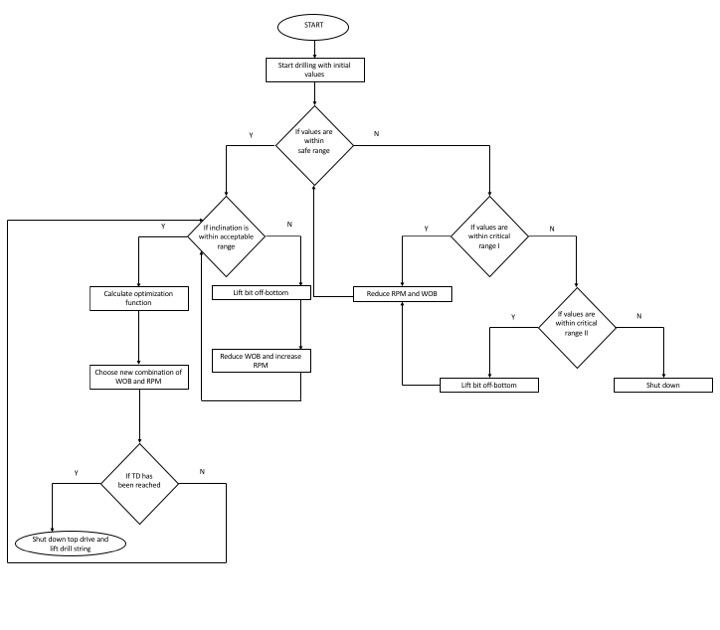
\includegraphics[width=1.0\textwidth]{figures/GeneralAlg.jpg}
\caption{Flow chart illustrating the general control algorithm}
\label{fig:algoflowchart}
\end{figure}


Figure (\ref{fig:algoflowchart}) shows how the drilling algorithm works step by step. When pressing the START button, the initial values for the control parameters are set, and drilling and continuous monitoring of key parameters start. The next step is to ensure that all parameters are within the safe operating range. If they are not, the algorithm will respond. If parameters are within the safe range, drilling continues and optimization can start. 

The purpose of the optimization function is to choose the best combination of control parameters to maximize the efficiency of the drilling operation. This procedure will continue until the desired depth has been reached. 

A way to monitor drilling efficiency is to measure the speed of drilling, or in other terms, the Rate of Penetration (ROP). ROP is a measure of depth drilled per unit time and maximizing this value will be crucial in carrying out an efficient drilling operation. 

\subsection{Drilling Optimization}
Maximizing ROP can be treated as an optimization problem. The goal of optimization is to maximize or minimize a given function by systematically choosing input values and calculating the value of the function. In more general terms, optimization is finding the best available value of a function given a defined domain. Applying the theory of mathematical optimization to this case, the goal will be to find the best available value of WOB and RPM to generate the highest possible ROP. The first step in this problem will be to define an optimization function.

There are different possible optimization functions, one of them is the concept of Mechanical Specific Energy. The function relates WOB, RPM, ROP and torque, and is a measure of how much energy is required to remove a unit volume of rock. Minimizing MSE is one way to maximize the ROP and consequently, the drilling efficiency. 

Another approach is to define a function which quantifies the amount of energy wasted in the system. It would be a function of the vibrations in the drill string as these are expected to be the largest cause of energy loss. Minimizing the energy waste would result in maximizing the useful energy and, thus, maximizing the drilling efficiency.

A third approach is to combine the two concepts introduced above. Such a function would improve drilling efficiency both by ensuring the least possible amount of energy is needed to remove the rock and by reducing the amount of energy wasted.

A further introduction to drilling optimization will be given to provide a deeper understanding of the choice of optimization function and algorithm.

\subsubsection{MSE Minimization}

A possible optimization function that can be used in this case is the function of Mechanical Specific Energy which is a measure of how much energy is required to remove a unit volume of rock and it is usually expressed in terms of drilling parameters such as weight on bit (WOB), torque, rate of penetration (ROP) and rotational speed (RPM). Choosing the optimum combination of controllable variables to minimize the MSE, will result in optimizing the drilling efficiency. 

MSE is defined by equation (\ref{eq:mse}).

\begin{equation}
\centering
   MSE = \frac{Total Energy Input}{Volume Removed}
\label{eq:mse}
\end{equation}

There are two forces acting on the bit during drilling: WOB (axial force) and torque (rotational force). MSE can be expressed in terms of these forces, as shown in equation (\ref{eq:msev}) and (\ref{eq:mset}). 

\begin{equation}
\centering
   MSE = \frac{Vertical Energy Input}{Volume Removed} + \frac{Rotational Energy Input}{Volume Removed}
\label{eq:msev}
\end{equation}

\begin{equation}
\centering
   MSE = \frac{WOB x \Delta h}{Area x \Delta h} + \frac{Torque x 2\pi x Numbers of rotations}{Volume Removed}
\label{eq:mset}
\end{equation}

Because the distance travelled by the bit is the ROP divided by the RPM, equation (\ref{eq:mset}) can be rearranged to give equation (\ref{eq:mser}).

\begin{equation}
\centering
   MSE = \frac{WOB}{Area} + \frac{2\pi x RPM x Torque}{Area x ROP}
\label{eq:mser}
\end{equation}

As shown in equation (\ref{eq:mser}), MSE is a function of drilling parameters that will be monitored continuously through the drilling process. Using MSE as an optimizing function is therefore a possible solution to ensuring an effective drilling operation. 

However, an important factor to consider is that MSE is not only a function of drilling efficiency, it is also a function of the type of rock that is being drilled through.

Instead of choosing WOB and RPM combinations randomly, experiments can be done to define a few regimes that will work well in the most common formations. This will be done to avoid trying out combinations that are unlikely to have good results. It is important to note that this is not a way to identify rock types, it is a way to make a better initial guess for the optimization algorithm.

A few different rock types will be selected based on what is most likely to encounter when drilling a well and they will have very different properties to cover a wider range of possibilities. Test drilling will then be performed to determine the best ranges of WOB and RPM for the different rock types. These ranges of values will be the main area where the algorithm looks for a good combination of control parameters. The tests will be conducted once the rig has been constructed and the system is ready to be tested.

\subsubsection{Vibration Minimization}

A second way to optimize the drilling efficiency is to minimize the waste of energy. When drilling, the goal is that all the energy provided by the top drive should be used to remove rock. However, a lot of the energy transforms into vibrations. To ensure that the operation is as efficient as possible, the goal will be to minimize the waste of energy.

Vibrational motion can be understood in terms of the conservation of energy. When the pipe is displaced from its center, some potential energy is stored in the pipe. When it is released and returns to its neutral state, its mass is accelerated and the potential energy is transformed into kinetic energy. The mass then decelerates and transfers the kinetic energy back to its potential. Oscillation of the drill string therefore amounts to transferring back and forth from kinetic energy to potential energy.

To quantify the amplitude of the vibrations, the amount of energy in the oscillation can be calculated. By using an accelerometer downhole, continuous measurements of the movement can be made and this will enable the calculation of the waste of energy through vibrations. 

The waste of energy can then be minimized by creating an optimization algorithm that uses the accelerometer measurements to monitor the vibration energy, and the control parameters to reduce the vibration amplitude.

\subsubsection{Borehole Verticality}

One of the main requirements of the rig is to be able to drill as vertically as possible which will be ensured by downhole sensors. A gyroscope and an accelerometer will be included in the same sensor and, although they are similar in purpose, they measure different things and together they provide accurate information about position and orientation.

The expected cause behind deviation is the occurrence of a tilted layer or encountering a new layer/rock inclusion with different rock properties. This may cause the bit to deviate from vertical position as it attempts to find the easiest path to drill.

To include a response to a change in inclination in the optimization function, a range of acceptable inclination values must be defined. This means that if the change in inclination is larger than a given value, the control system will respond by lifting the bit a pre-defined length and resume drilling with lower WOB and the same or higher RPM.


\subsection{Algorithm for finding Global Maximum of Optimization Function}

As explained previously, the aim of the model is to continuously ensure the safety of the equipment and personnel, as well as improve drilling efficiency by using an optimization algorithm. There are several optimization methods that can be used in this situation and a review of three different possibilities will be provided below.

\subsubsection{Gradient Descent and Gradient Ascent}

The Gradient Descent method, also known as Steepest Descent, is a first order iterative optimization algorithm. Given a function defined by different sets of parameters, the Gradient Descent method starts with a set of initial parameter values. By solving the problem iteratively, for each step of iteration a new set of variables is chosen and we move towards a minimum point to minimize the given function. In other words, we take steps proportional to the negative of the gradient. 

Gradient Descent is an algorithm used to find the nearest minimum point. Gradient Ascent is the opposite. The same procedure is used, but in this case, the nearest maximum is approached by moving proportionally to the positive of the gradient. This a sort of Hill Climbing solution method. 

Gradient Descent and Gradient Ascent are excellent choices if there is only one maximum or minimum point. In this problem, the number of maximum or minimum points is unknown. 
Both Gradient Descent and Gradient Ascent use local searches and the risk of getting stuck in a local optimum or minimum is therefore large. This means that the algorithm is tricking us to believe the given set of variables is the best solution to optimize the drilling operation. In reality, there exists a set of other parameters that may lead to better drilling performance. Our main goal is to optimize the drilling operation without getting stuck in a local maximum or minimum and try to find the global maximum or minimum, the gradient descent/ascent method is therefore not the optimal choice.


\begin{figure} [H]
\centering
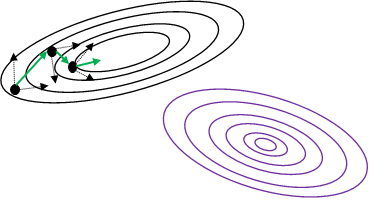
\includegraphics[width=0.7\textwidth]{figures/gradientdescentmethod.png}
\caption{Illustration of the gradient descent method}
\label{fig:gradientdm}
\end{figure}

As illustrated in figure (\ref{fig:gradientdm}), the Gradient Ascent method uses a local search to find the optimum point of the function. The risk is that it finds a local optimum, black circles, instead of a global optimum, purple circles.

\subsubsection{Simulated Annealing}

Simulated Annealing (SA) is a probabilistic method to estimate the global maximum of a given problem. The method uses the same approach as Hill Climbing, but it occasionally selects random sets of variables and allows the algorithm to use solutions that are worse than the current. By doing this, the algorithm avoids a premature convergence which occurs when the algorithm thinks the chosen variables are optimal (stuck in a local optimum), but the solution is actually a suboptimal. 

Compared to the method of gradient descent/ascent, this method eliminates the risk of getting stuck in a local optimum point which is positive. However, it allows using solutions that are worse than the current one which might cause the method to be less effective than the steepest descent. The benefit of reaching a global optimum versus only a local optimum should be compared to the drawback of spending time drilling in a regime that is worse than the current one.

Figure (\ref{fig:siman}) illustrates how the Simulated Annealing algorithm chooses random sets of variables (x1, x2, x3…) to determine the location of the global maximum and how it allows using solutions that are worse than the current one (x4 and x5 vs x3).

\begin{figure} [H]
\centering
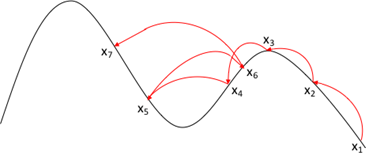
\includegraphics[width=1.0\textwidth]{figures/siman.png}
\caption{Illustration of the simulated annealing method}
\label{fig:siman}
\end{figure}

\subsubsection{Genetic Algorithms}

Genetic Algorithms (GA) is a method inspired by Charles Darwin’s Theory of Natural Selection and is used to solve both constrained and unconstrained optimization problems. Genetic Algorithms start with randomly selected variables in the initial generation of candidate solutions that are tested against the objective function. From the initial generation, the best performing variables are favored and selected to reproduce. 

There are two possible outcomes for the next generation. The first one is called a crossover and involves two favorable variables from the previous generation combining to create a new generation of population. The previous generation can be referred to as parents and the new one as children. 

The second one is called a mutation. Here, one favorable parent from the previous generation is combined with one favorable child from the current generation to create an individual for the new generation. Using mutations helps to find the global optimum point and avoids the risk of the algorithm getting stuck in a local optimum. 

For each new generation, individuals that are evolving towards an optimal solution of the function will be used as parents for the next generation. This process continues until the desired optimization is established. 

Figure (\ref{fig:genetic}) shows the evolution of the different generations and how the algorithm differentiates between local optimums (blue circles) and the global optimum (red circles). The favorable variables, the ones closest to a local or global optimum, are shown as colored triangles and the desired optimum is the black triangle.

\begin{figure} [H]
\centering
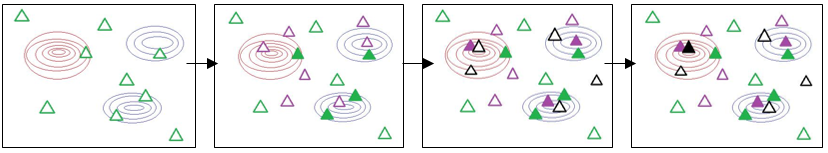
\includegraphics[width=1\textwidth]{figures/genetic.PNG}
\caption{Illustration of the concept of genetic algorithms}
\label{fig:genetic}
\end{figure}


The benefit of using a Genetic Algorithm is that the risk of getting stuck in a local optimum point is eliminated. The problem is that it requires trying out many different combinations of parameters for every generation of solutions and this may be too time-consuming for a small-scale drilling operation.

\subsubsection{Proposed Solution}

The Gradient Descent method will not be used because the risk of getting stuck in a local optimum point is large compared to the other two methods. Both the Genetic and Simulated Annealing methods are good choices, but they are time consuming since they must test many control parameter combinations before selecting the optimum solution. The main difference between the two methods is that the Genetic Algorithms will test several combinations before moving to the next step, while Simulated Annealing will test one combination for each step. Because many different rock types may be encountered when drilling, the range of the control parameters is expected to be large and the Genetic Algorithm is therefore preferred.

To solve this optimization problem, the Genetic Algorithm method has been chosen, but it has been simplified in order to save time. The optimization function will be a combination of MSE and vibration energy, and the aim will be to minimize it.

\begin{figure} [H]
\centering
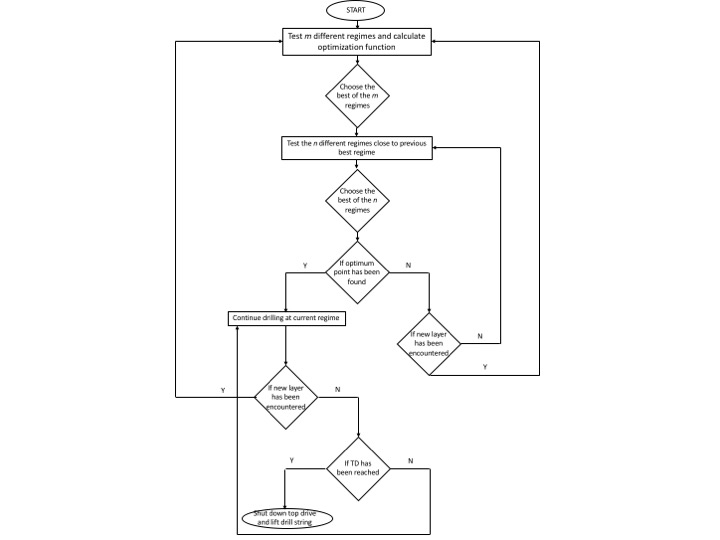
\includegraphics[width=1.0\textwidth]{figures/OptAlg.jpg}
\caption{Flow chart of the optimization algorithm}
\label{fig:optialgo}
\end{figure}

The first step is to choose m combinations of input values within the range of data determined from the testing of rock samples. Drilling will continue at the regime that resulted in the optimum value for the optimization function. Next, the search range is reduced and moved close to the previous best solution. n new combinations of parameters are tested and drilling continues with the best combination. 

A criterion to determine whether the drilling efficiency is satisfactory must be defined. A possibility is to use MSE. When the difference between the MSE at the previous regime and the MSE at the current regime is small enough, the control parameters can be assumed to be optimal. The critical value y will be determined during the testing phase. This combination of parameters will be used until a new layer is reached.

A possible way to identify a new layer is to monitor how much the ROP changes. When the change in ROP is sudden and large, it may be assumed that a new layer is encountered and the optimization process must start again from the first step.

The algorithm is illustrated in figure (\ref{fig:optialgo}).

In this year’s competition, a pilot hole will be pre-drilled using the same bit as the on-site test and must be less than 1 in deep. This will not require any optimization, so a simpler version of the drilling algorithm will be used, as shown in figure (\ref{fig:pilothole}).

\begin{figure} [H]
\centering
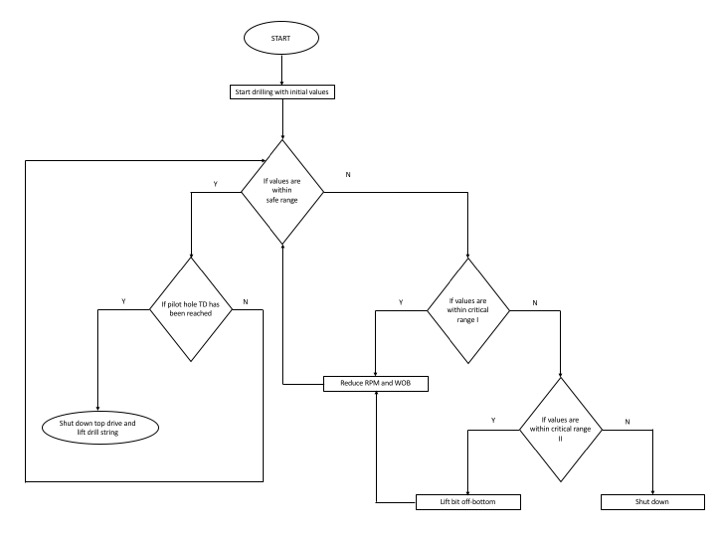
\includegraphics[width=1.0\textwidth]{figures/PilotHole.jpg}
\caption{Flow chart for the pilot hole algorithm}
\label{fig:pilothole}
\end{figure}













\newpage
\section{Control System}
\label{sec:8}
The drilling operation will be controlled by a programmable logic controller (PLC) which will receive analog input from downhole and surface sensors, digitalize the data so that the control algorithm can be applied, and then transmit analog signals to the motor controllers to adjust the control parameters. The PLC can be programmed using Simulink which is integrated in Matlab, enabling the incorporation of Matlab algorithms. 

\numberwithin{equation}{section}
\numberwithin{figure}{section}
\numberwithin{table}{section}

The sensors included in the control system measure key drilling parameters. Vibration, inclination, azimuth and bit temperature will be monitored downhole, while RPM, torque, pressure, flow and the position of the ball screw are all surface measurements. The measurements will continuously be transmitted to and processed by the PLC which will in turn send signals to the hoisting motor, top drive and pump to adjust the WOP, RPM and flow rate.

\begin{figure} [H]
\centering
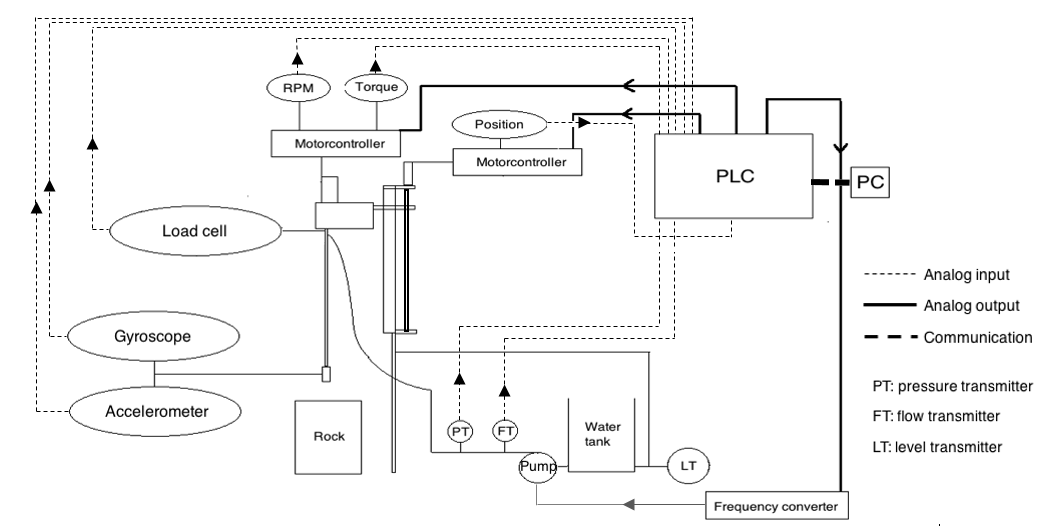
\includegraphics[width=1.0\textwidth]{figures/controlsystemflc.png}
\caption{Control System Flow Chart}
\label{fig:controlsystemflc}
\end{figure}

\subsection{Measurement and Sensors}

The analog data from the sensors will be transmitted to the PLC through wires. The wires will be placed inside the drill pipe, along the pipe wall. Wireless transmission was considered, but the water in the drill pipe, the thickness of the pipe wall and the rotation of the string, may cause noise which makes the data unreliable. 

No sensor is perfect, and even sensors from the same manufacturer can yield different readings. In addition to this, the sensors may change response if they are subjected to varying conditions like heat, humidity and shocks. Calibrating the sensors will therefore be of great importance to build and operate a complete automated drilling system. 

There are different methods of calibration, all varying in complexity \cite{ada}. The one-point method is the simplest method and is used when the sensor calibration is scaled and only sensor offset needs to be corrected. It is done by taking a measurement with the sensors, comparing the measurement with the reference standard, calculating the offset by subtracting the sensor reading from the reference reading and finally adding the offset to every sensor reading in the code.

The second method is two-point calibration. It is more complex than the one-point method, but can be applied to both scaled and raw sensor output. This method rescales the output and corrects both slope and offset errors. It can be used in cases where the output is known to be relatively linear. This method of calibration is performed by taking two measurements from the sensor: one near the low end and one near the high end. These measurements must then be repeated with the reference instrument and the corrected value can then be calculated by using equation (\ref{eq:twopoint})


\begin{equation}
\centering
   Corrected value = \frac{(raw Value - Raw Low Value) x Reference Range}{Raw Range}+Reference Low Value
\label{eq:twopoint}
\end{equation}

The last method is the multi-point curve fitting calibration. This is the most complex method and is used for sensors that are not linear. This can be done using Excel or similar spreadsheet programs. 

The need for calibration will be different for every sensor. The downhole sensors may experience large changes in conditions while the surface sensors will not, and they will therefore require a different type of calibration. 

Calibration will be performed during the testing period to determine reference standards for all sensors. Additional calibration will need to be done while drilling in case the sensor response changes. 

\subsubsection{Direct Output from Motors}
The RPM and the torque are direct outputs from the top drive motor. 
ROP will be estimated from the direct position output of the hoisting motor.

\subsubsection{Surface Sensors}
The following sensors are the sensors that will make measurements at surface. Some of these measurements will approximate downhole measurements.

\paragraph{Load Cell}
A load cell is a transducer which converts force into a measurable electrical output. It measures the tension in the drill string at surface, but the WOB can be estimated by suspending the bit off bottom. As the bit is lowered and touches bottom, the hook load decreases by an amount equal to the WOB. It will be placed at the top of the drill string.

\paragraph{Pressure Transducer}
A pressure transducer converts pressure into an analogue electrical signal. The main benefit of including this sensor is to be able to estimate the pressure in the different components of the circulation system.

\paragraph{Flowmeter}
A flowmeter is an instrument that measures the volumetric flow rate of a fluid, in this case the flow rate of the drilling fluid out of the pump. Because the pump pressure is expected to be high, the use of a flowmeter must be re-evaluated during the test phase. If the flowmeter cannot be used, the flow rate can be estimated from the rotational speed and cylinder size of the piston pump.

\subsubsection{Downhole Sensors}
\paragraph{Accelerometer and Gyroscope}
The accelerometer and the gyroscope will be included in the same sensor in the BHA. It will be placed over the constriction.

The accelerometer measures vibration, or acceleration, in the BHA. Its main use will be monitoring the amplitude of the vibrations.

The gyroscope provides estimates of inclination and azimuth by measuring the angle of deflection from the vertical. As the verticality of the borehole is an important factor during the competition, this will be a valuable measurement.

Temperature will also be measured using this sensor. The purpose of measuring the temperature is to avoid overheating the bit which can reduce the efficiency of drilling and damage the bit itself.

\subsection{Response Time}
The response time of measurements, data aggregation and control algorithms, will be estimated to ensure real-time control of the drilling process.

The response time of sensors will be determined experimentally as the theoretical approach requires thorough knowledge of the design of the sensor, its construction details, the properties and geometries of the sensor’s internal material as well as knowledge of the properties of the medium surrounding the sensor \cite{hash}.

Data aggregation will in this case consist of processing the data in the PLC and transmitting it to the PC.

Finally, the response time of the control algorithm needs to be estimated.


\newpage
\section{Data Handling and Display}
\label{sec:9}
The data gathered from the various sensors are transmitted through a PLC into a computer. The PLC converts the analog signals from the sensors into digital signals, so it is readable for the computer. A set of different parameters, either direct output from sensors or output from the computer, are monitored at all time to ensure safety and to optimize the drilling operation. 

\numberwithin{equation}{section}
\numberwithin{figure}{section}
\numberwithin{table}{section}

Simulink, which is a graphical programming environment for simulation, modelling and multi-domain dynamic system analysis, will be used to display parameters such as WOB, RPM, torque, ROP, MSE, flowrate, pump pressure, vibrations and inclination, on screen in real time. The data display will also notify the user of any parameters outside the safe operating range. A message about which safety measure the rig is taking will also appear on the screen. This will give an overview of the drilling operation at any time.

The accelerometer and gyroscope provide measurements that enable the monitoring of inclination, azimuth and position of the drill string in the formation. A possibility is to use the output of these sensors to create a 3D-plot of the wellbore in real time. 

Because the idea behind the drilling algorithm is to be able detect new layers, air pockets and drilling dysfunction, an illustration of where this changes occur could be displayed in the 3D-plot as well. The main purpose of this is to give us a live update of the wellbore and give a better understanding of the well path and the medium that is drilled in. 

\begin{figure} [H]
\centering
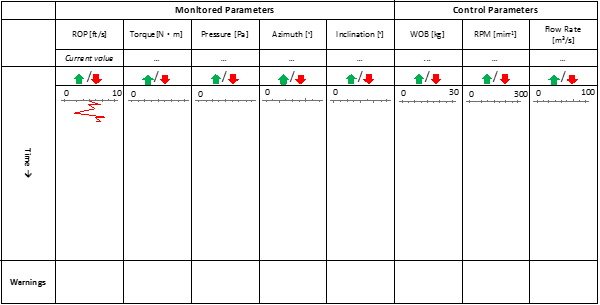
\includegraphics[width=1.0\textwidth]{figures/datadisplay.png}
\caption{Data Display 1}
\label{fig:datadisplay}
\end{figure}

\begin{figure} [H]
\centering
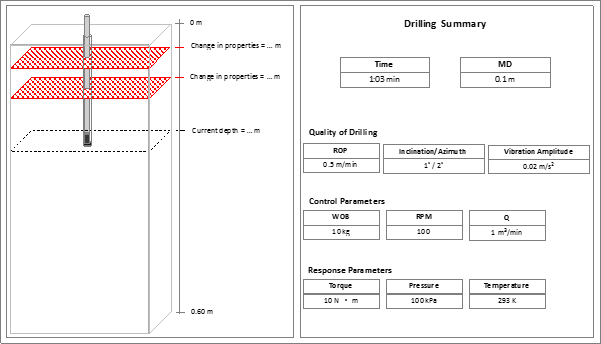
\includegraphics[width=1.0\textwidth]{figures/datadisplay2.png}
\caption{Data Display 2}
\label{fig:datadisplay2}
\end{figure}



\newpage
\section{Cost Estimate and Funding Plan}
\label{sec:10}
The cost of the rig and materials for 2016-2017 Drillbotics competition is limited to US\$ 10,000. The preliminary budget is shown in table (*), where all expected materials to be purchased are listed. Components that are already owned by the university or borrowed from companies are not included in the total expenses as they are free of cost.  

As of now the total expenditures will be covered by funding from the Petroleum Institute at NTNU. However, the goal for the coming months will be to attempt to get funding from relevant technology companies. We will try to implement innovative technology inspired by other industries, which can make it possible to get in touch with a wider range of companies. This can be companies that are working with control systems, sensors, vibration analysis etc. 

\begin{table} [H]
    \centering
    \caption{Cost Estimate}
    \begin{tabular}{p{4,5cm} p{3cm} p{1,5cm} p{2cm} p{2,5cm}}
        \large{Description} & \large{Cost per Unit} & \large{Amount} & \large{Unit} & \large {Total Cost} \\ \hline \hline
        \textit {\large{Rig structure}} \\
        Hollow section steel pipe (50mmx50mm) & &17.9 & m \\
        Hollow section steel pipe (50mmx80mm) & & 0.7 & m \\
        Hollow section steel pipe (100mmx40mm) & & 0.7 & m \\
        Adjustable plate (600mmx600mm) & & & m$^2$ \\
        Hinge & 200 & 2 & & 400 \\
        Table top (wood) & 300 & 2 & & 600 \\
        Caster & 120 & 6 & & 720 \\ \hline
         \textit {\large{Hydraulic System}} \\
        Pump (HAWK HC980A) & & 1 & & Owned \\
        Hose & 370 & 2.5 & m & 925 \\
        Safety valve & 400 & 1 & & 400 \\
        Swivel (3/8 in) (TESS) & 1,940 & 1 & & 1,940 \\ \hline
        \textit {\large{Linear Motion and Rotating Equipment}} \\
        Linear roller guide rail & 938.8 & 2 & & 1,877.5 \\
        Wagon for carriage & 686.9 & 2 & & 1,373.8 \\
        Ball screw system (MBA20-D-comp) & 3,294.4 & 1 & & 3,294.4 \\
        Top drive motor & & 1 & & \\
        Hoisting motor & & 1 & & \\ \hline
        \textit {\large{Sensors}} \\
        Accelerometer, gyroscope and temperature sensor & 70 & 1 & & 70 \\
        Load cell & & & & Owned \\
        Flowmeter \\ \hline
        \textit {\large{Other}} \\
        Machining/raw materials \\
        Electrical cables \\
        Coupling (swivel to drill pipe) \\
        Drill pipe & 200 & 3 & & 600 \\
        Tool joint & 300 & 1 & & 300 \\
        PLC & & 1 & & Provided by ABB \\
        Computer & & 1 & & Owned \\ \hline
        
         
        
    \end{tabular}
    \label{tab:sumpressure}
\end{table}


\newpage
\bibliography{biblio}

\newpage
\pagenumbering{Alph}
\appendix
\section*{Appendix}

\appendix
\section{Engineering Drawings} \label{App:AppendixA}

\begin{figure} [H]
\centering
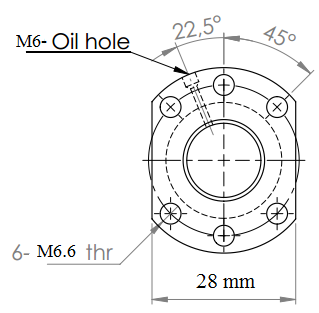
\includegraphics[width=0.6\textwidth]{figures/MechBS1}
\caption{Ball screw nut} \cite{aluflex}
\label{fig:MechBS1}
\end{figure}

\begin{figure} [H]
\centering
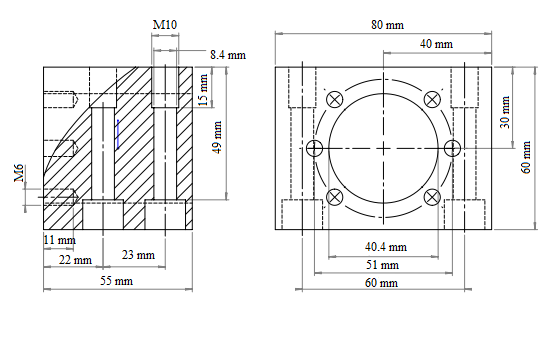
\includegraphics[width=0.8\textwidth]{figures/MechBS3}
\caption{Ball screw nut bracket MGD25} \cite{aluflex}
\label{fig:MechBS2}
\end{figure}


\begin{figure} [H]
\centering
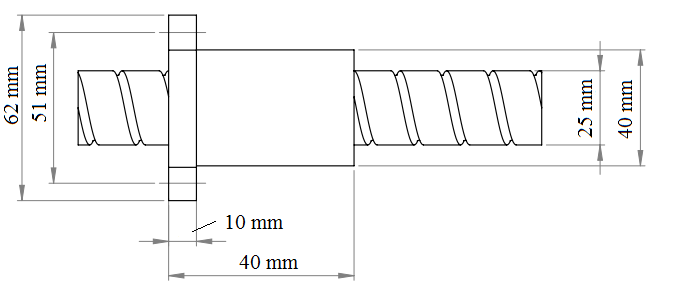
\includegraphics[width=0.8\textwidth]{figures/MechBS2}
\caption{Ball screw (MBA20-E-Comp)} \cite{aluflex}
\label{fig:MechBS2}
\end{figure}


\begin{figure} [H]
\centering
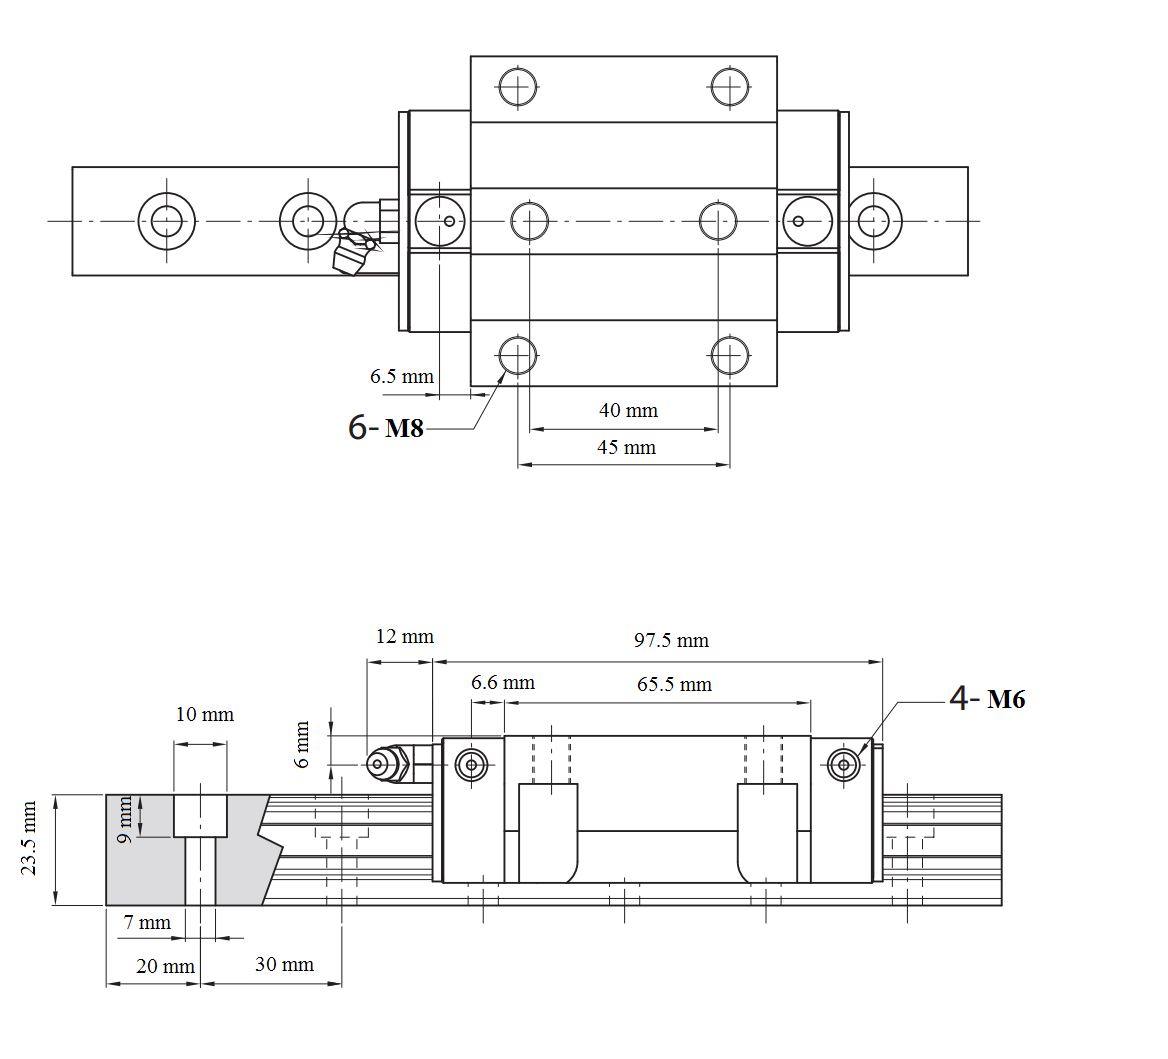
\includegraphics[width=0.8\textwidth]{figures/MechLBG1}
\caption{Complete linear roller guide package (MSR25 E) } \cite{Aluflex_LRG}
\label{fig:MechLRG1}
\end{figure}



\begin{figure} [H]
\centering
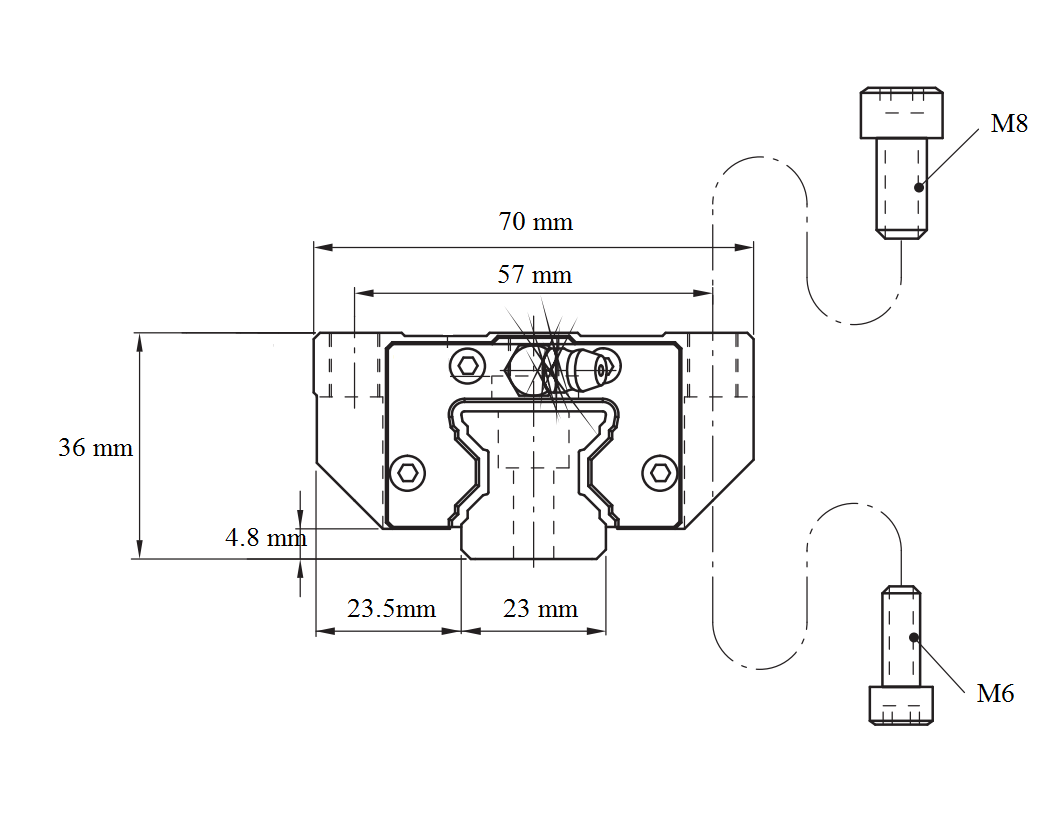
\includegraphics[width=0.8\textwidth]{figures/MechLBG2}
\caption{Linear roller guide carriage} \cite{Aluflex_LRG}
\label{fig:MechLRG2}
\end{figure}

\begin{figure} [H]
\centering
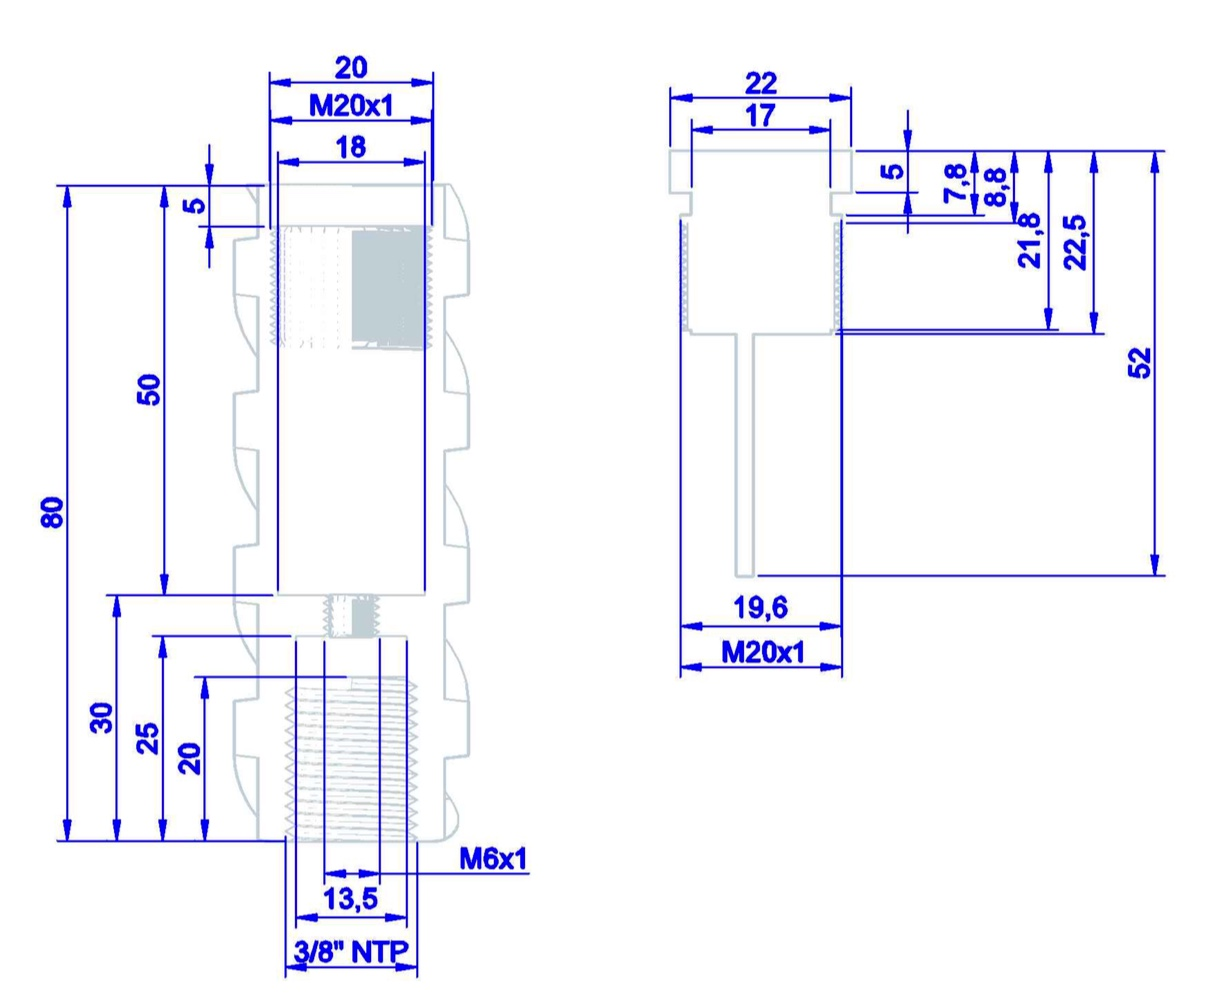
\includegraphics[width=0.8\textwidth]{figures/stabdim}
\caption{Side cut of stabilizer on the left hand side and sensor plate to be placed inside BHA on the right hand side. All dimensions in mm} 
\label{fig:StabDim}
\end{figure}

\newpage
\begin{figure} [H]
\centering
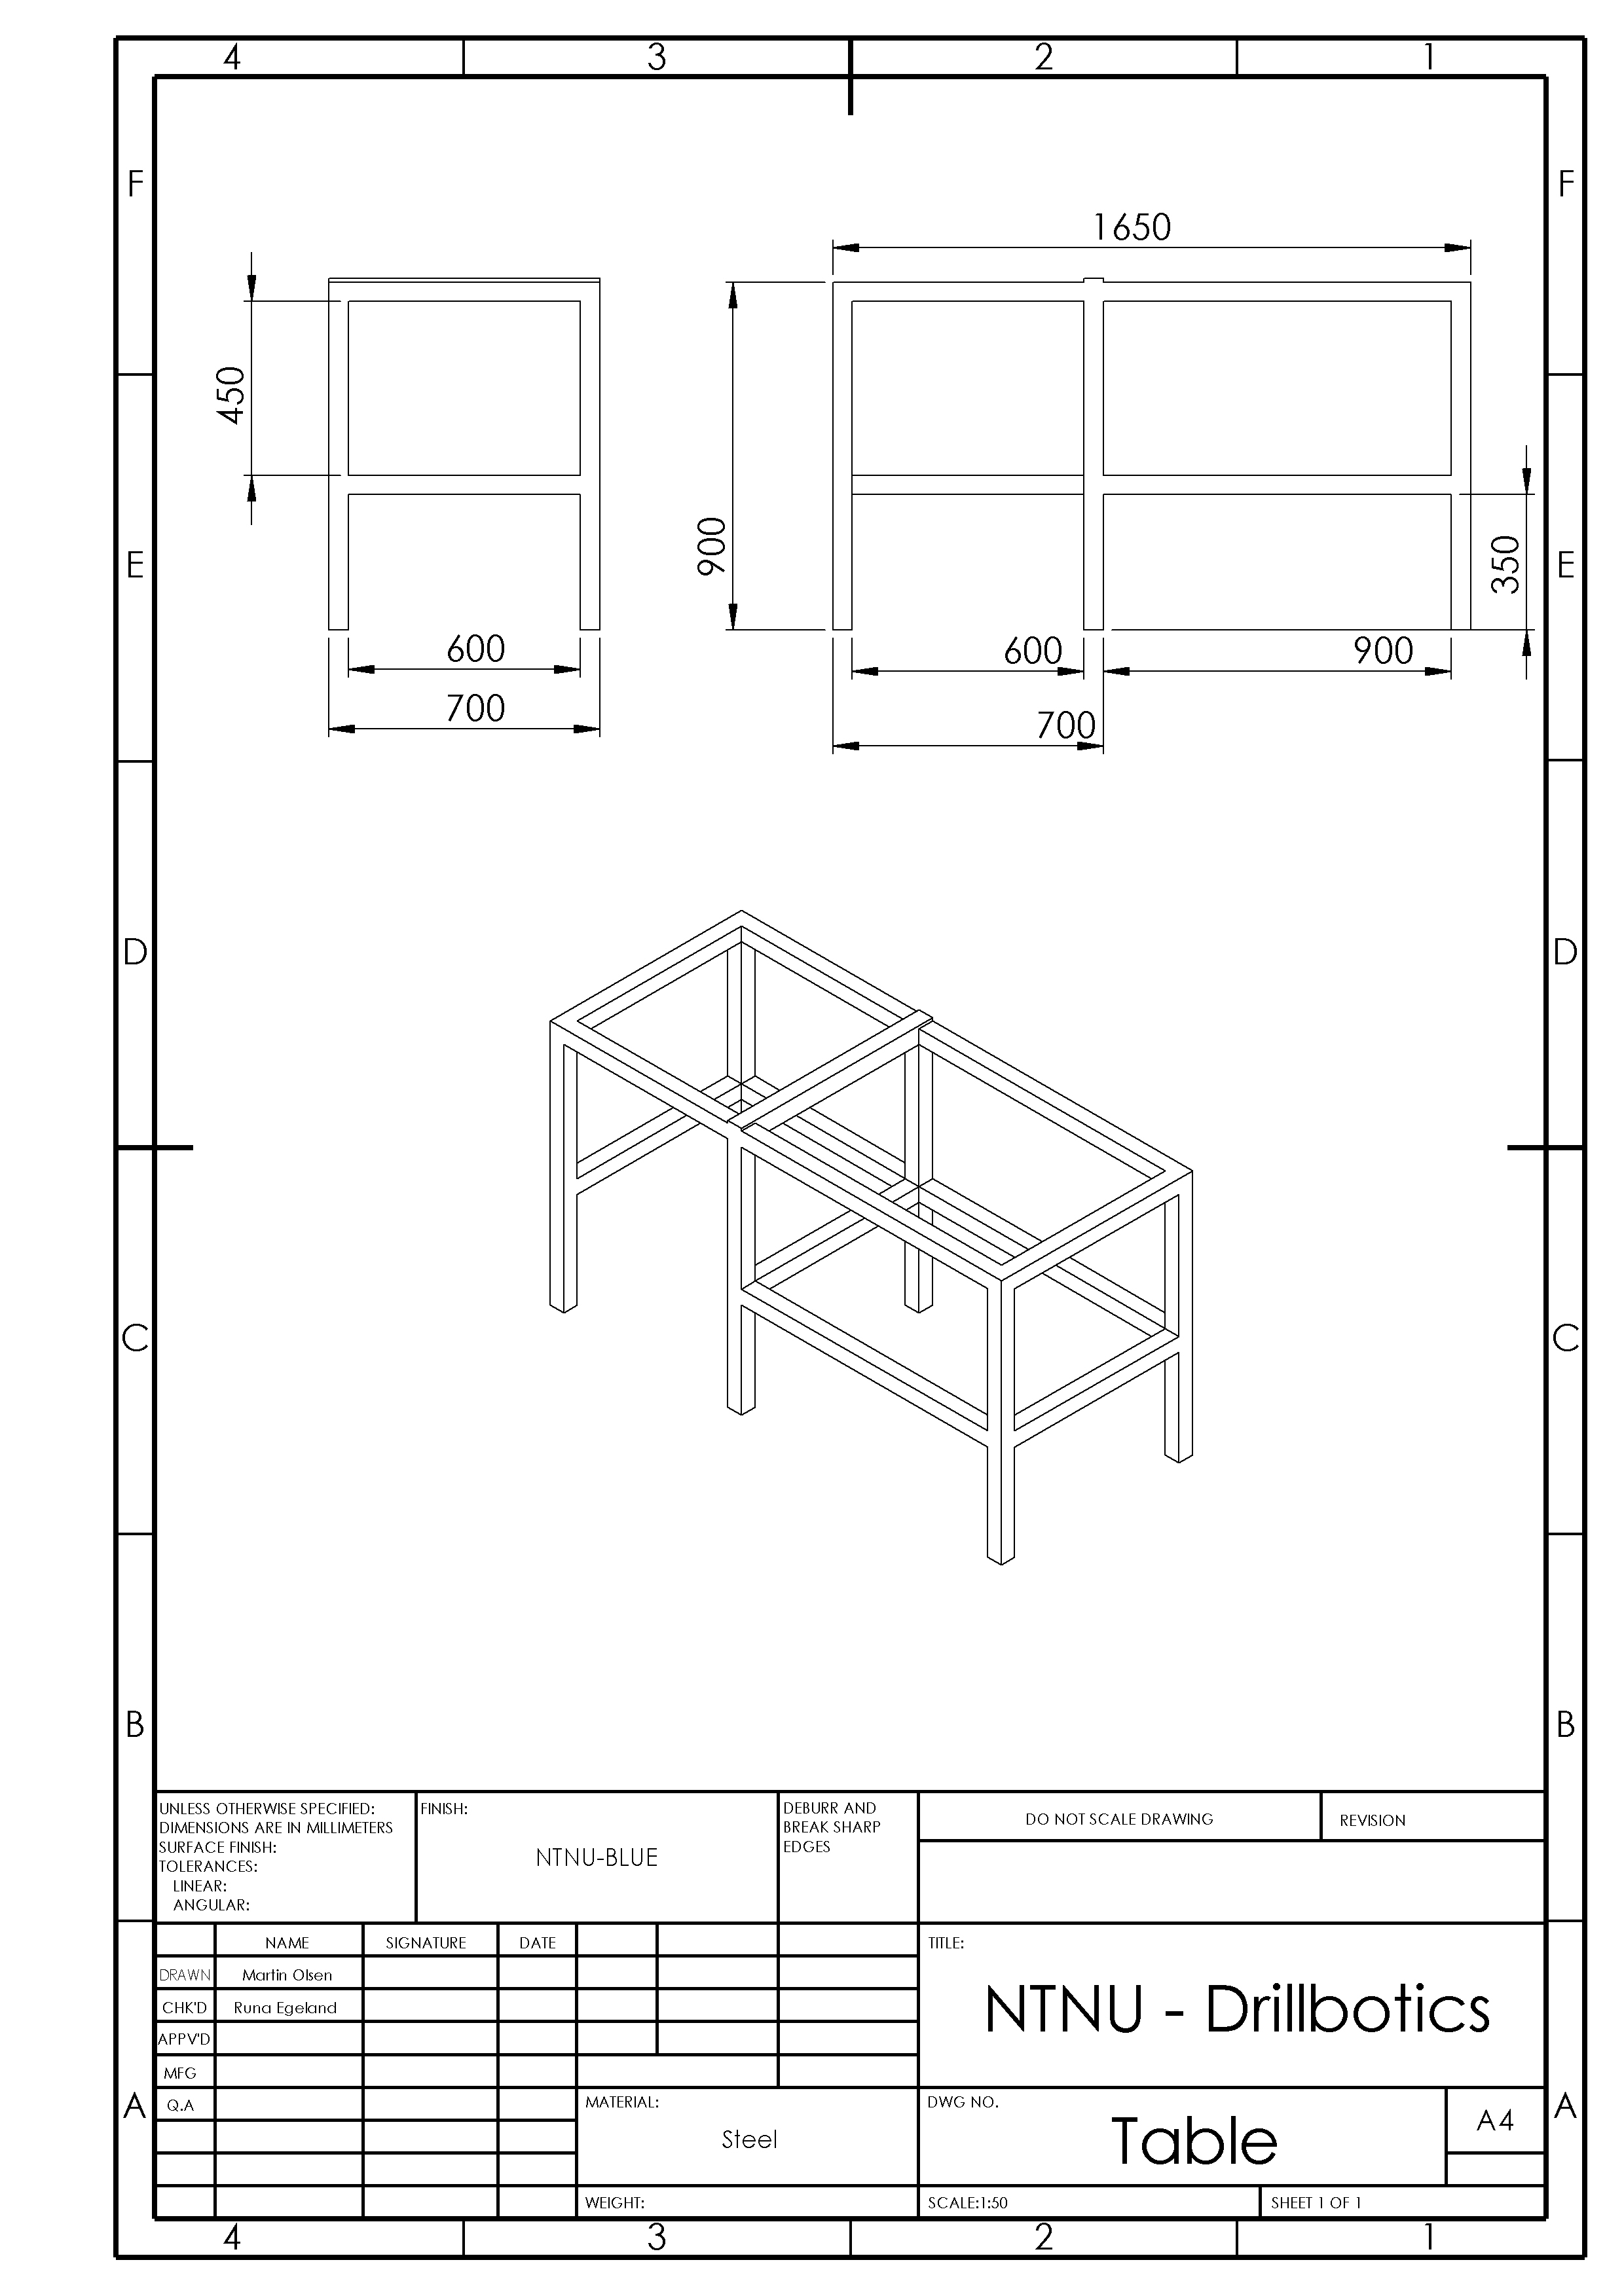
\includegraphics[width=1.0\textwidth]{figures/mechdrawings/Table.JPG}
\caption{Substructure of Rig. All dimensions in mm} 
\label{fig:table}
\end{figure}

\newpage
\begin{figure} [H]
\centering
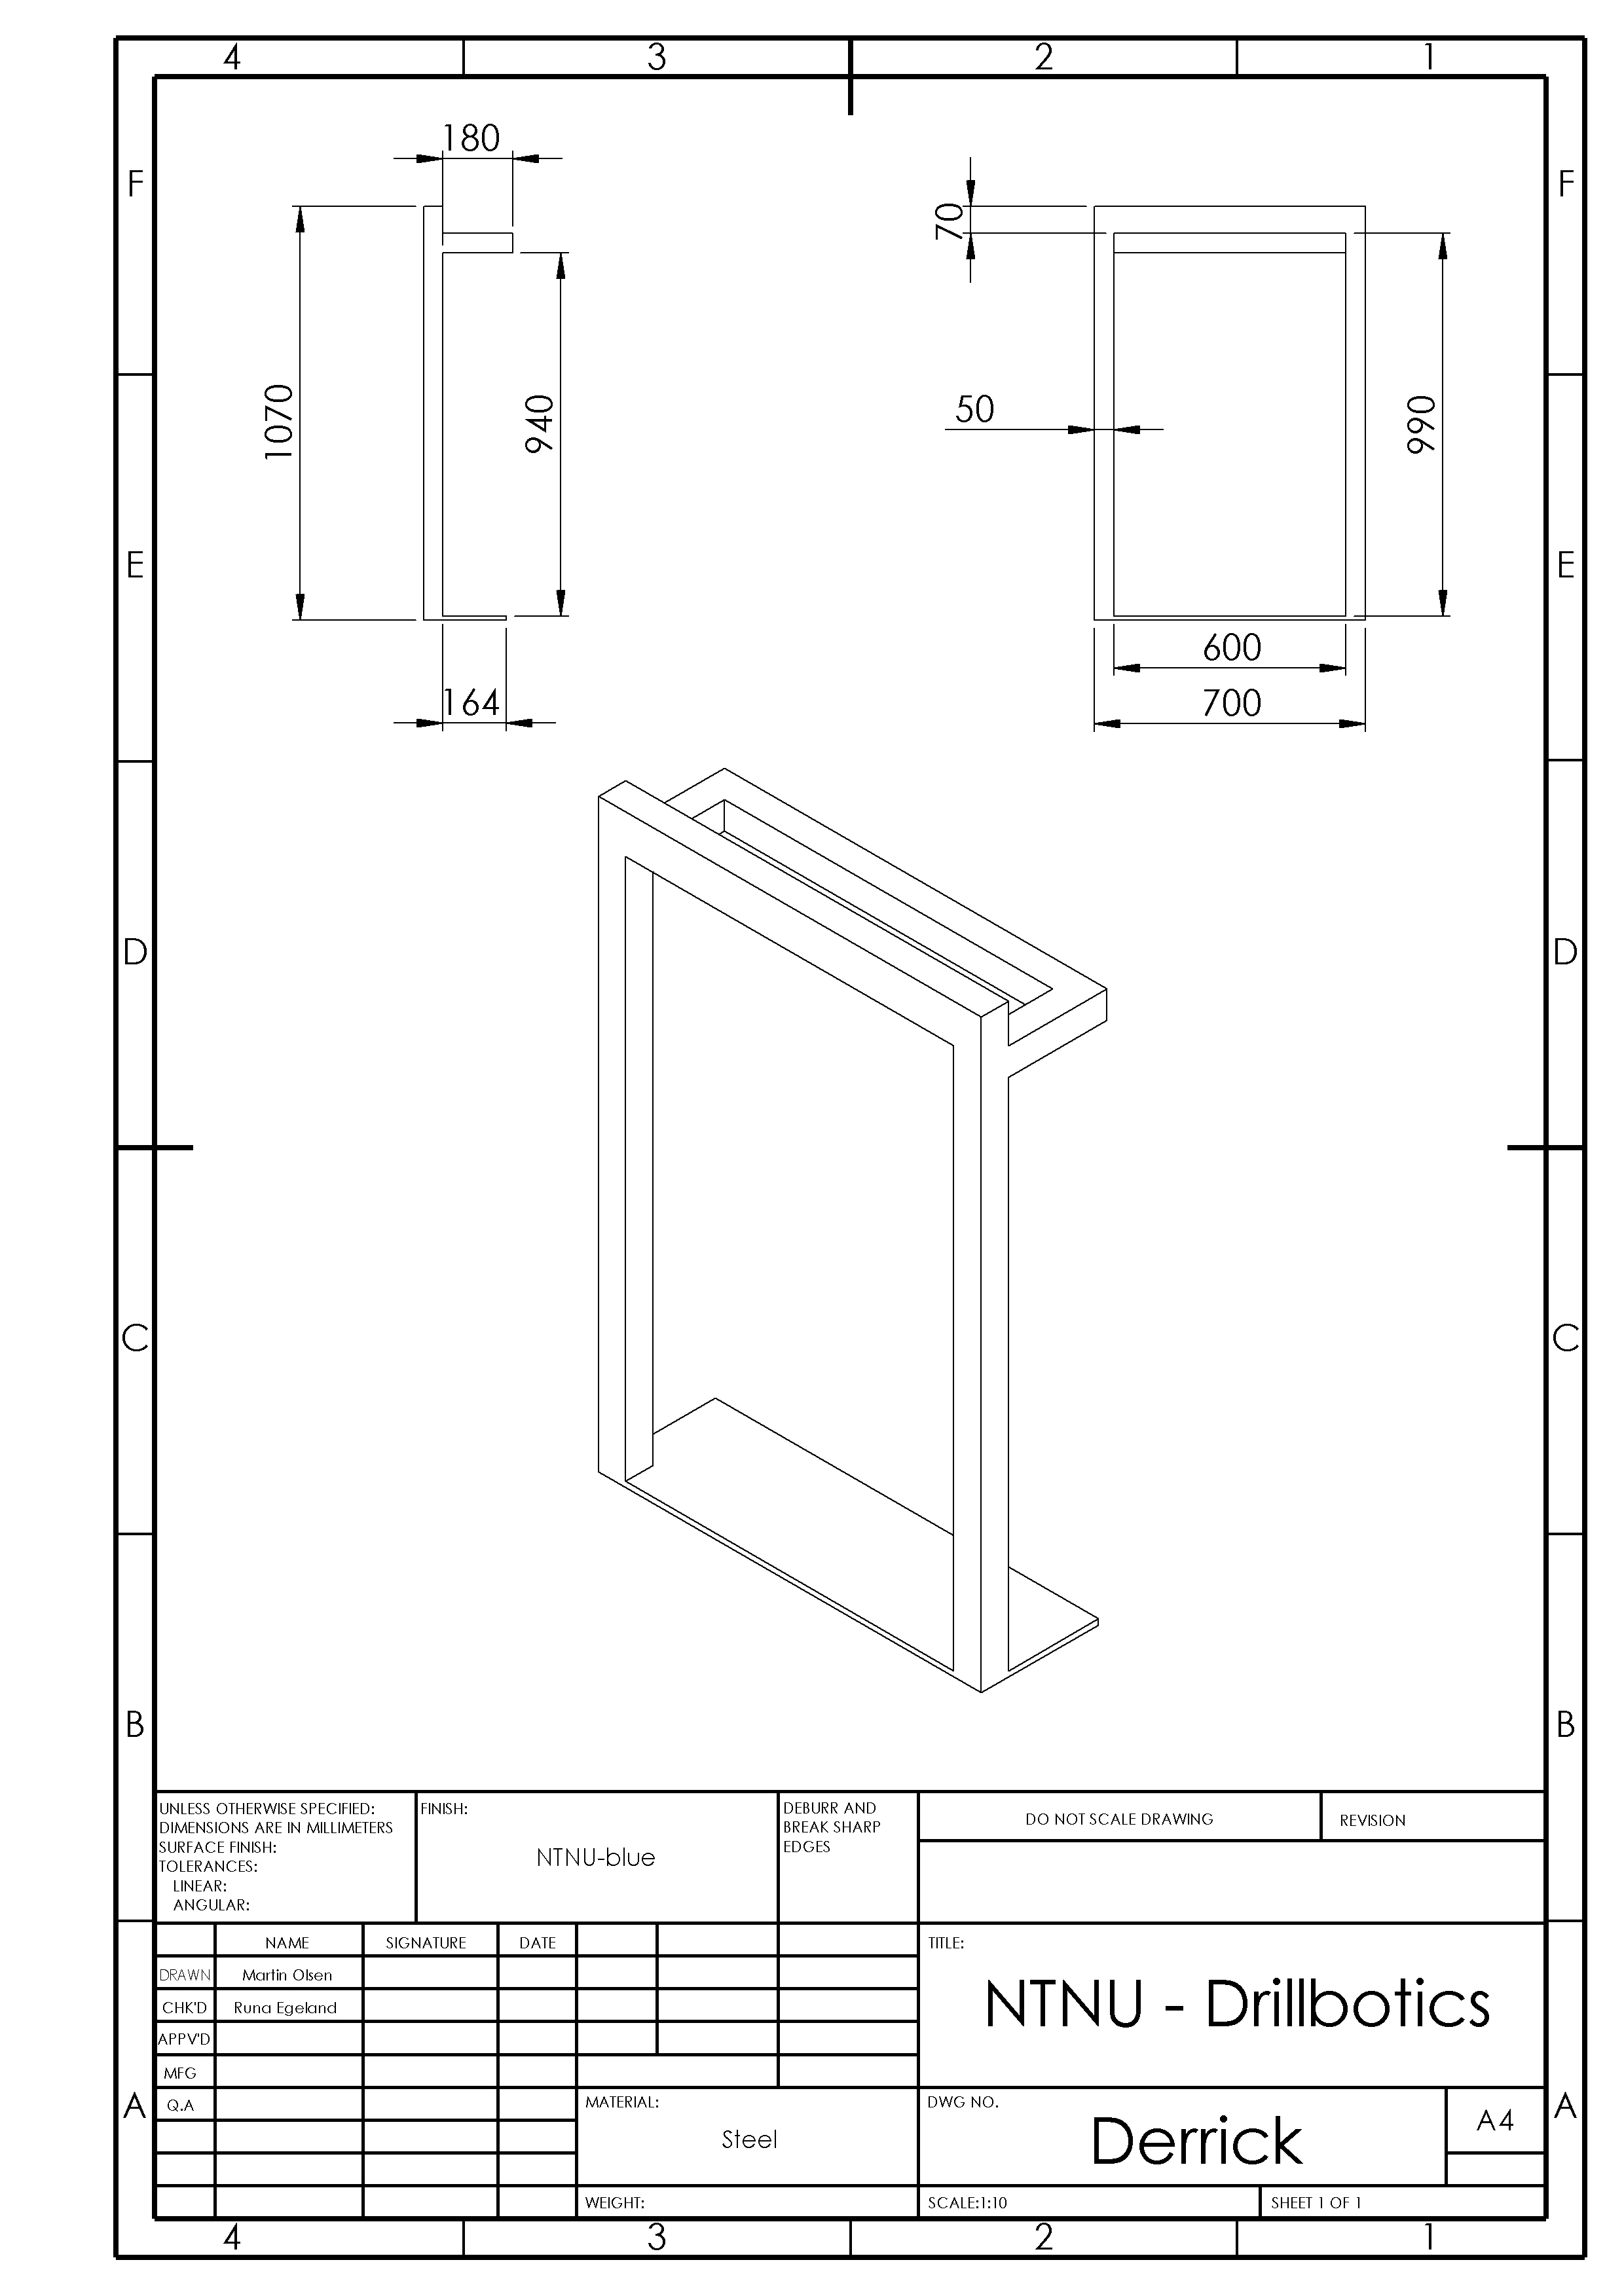
\includegraphics[width=1.0\textwidth]{figures/mechdrawings/Derrick.JPG}
\caption{Derrick. All dimensions in mm} 
\label{fig:Derrick}
\end{figure}

\newpage
\begin{figure} [H]
\centering
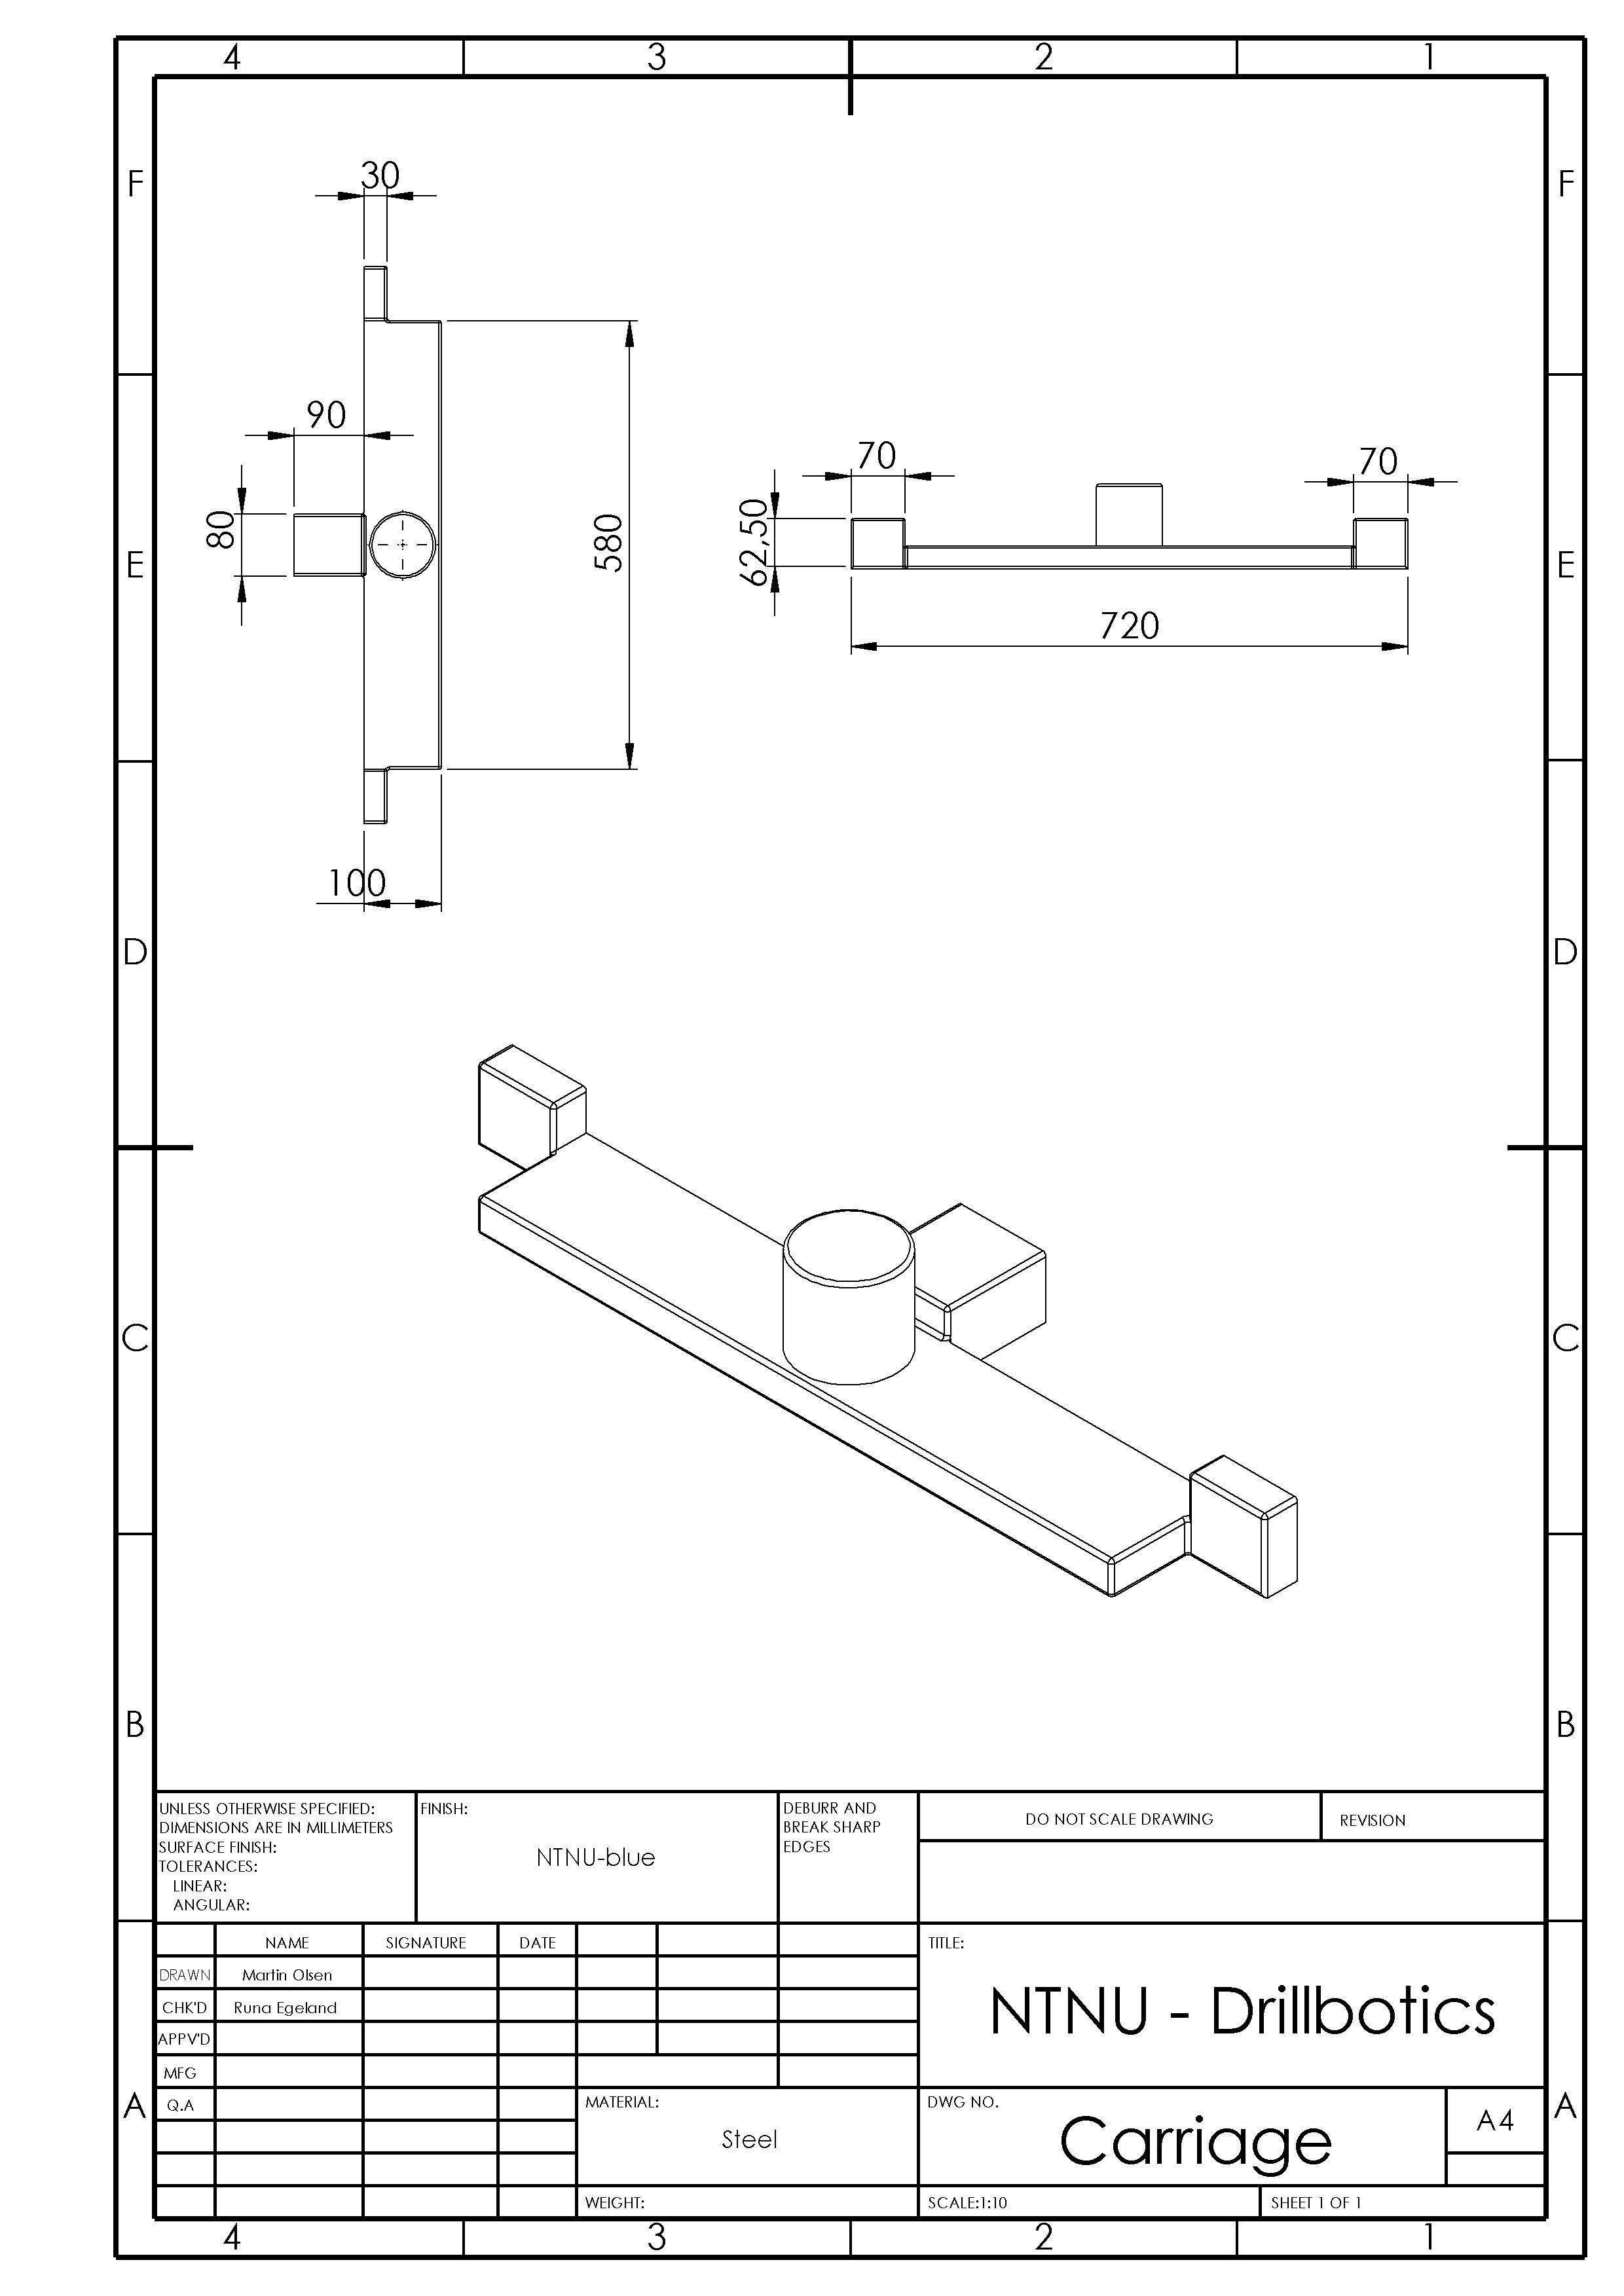
\includegraphics[width=1.0\textwidth]{figures/mechdrawings/Carriage.JPG}
\caption{Carriage. All dimensions in mm} 
\label{fig:Carriage}
\end{figure}

\newpage
\begin{figure} [H]
\centering
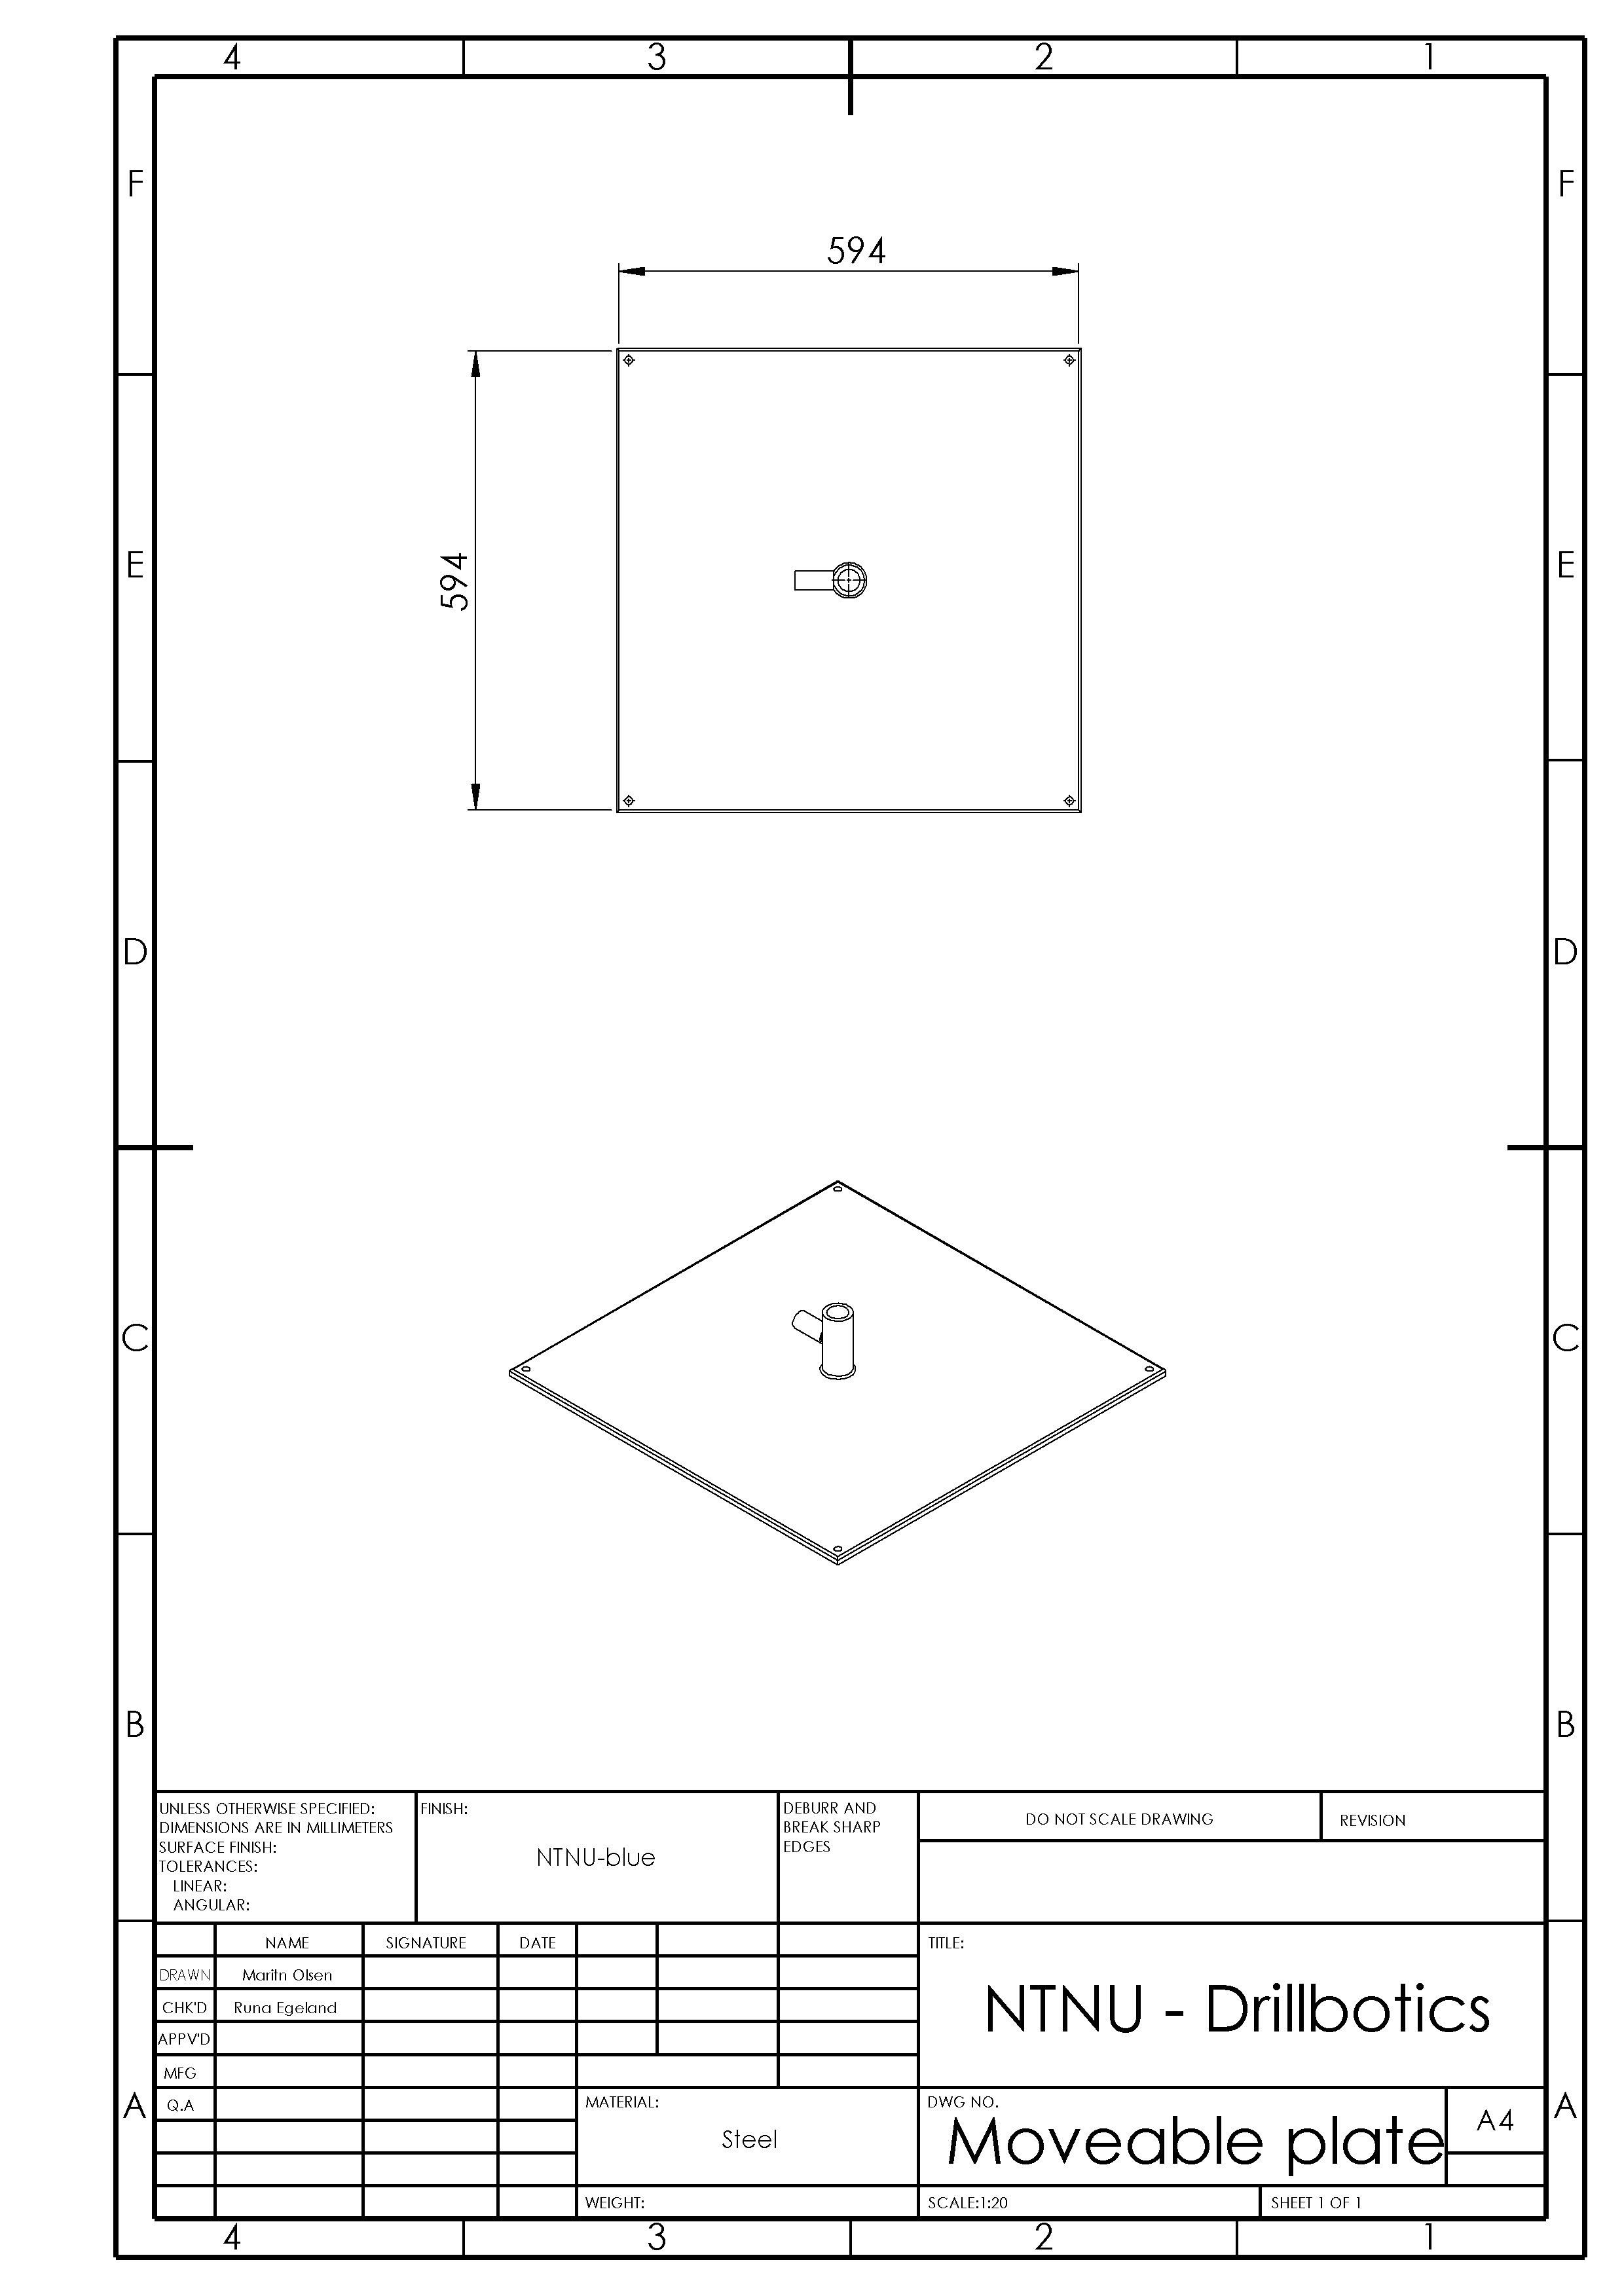
\includegraphics[width=1.0\textwidth]{figures/mechdrawings/Moveableplate.JPG}
\caption{Moveable Plate with Riser. All dimensions in mm} 
\label{fig:riserplate}
\end{figure}

\newpage
\begin{figure} [H]
\centering
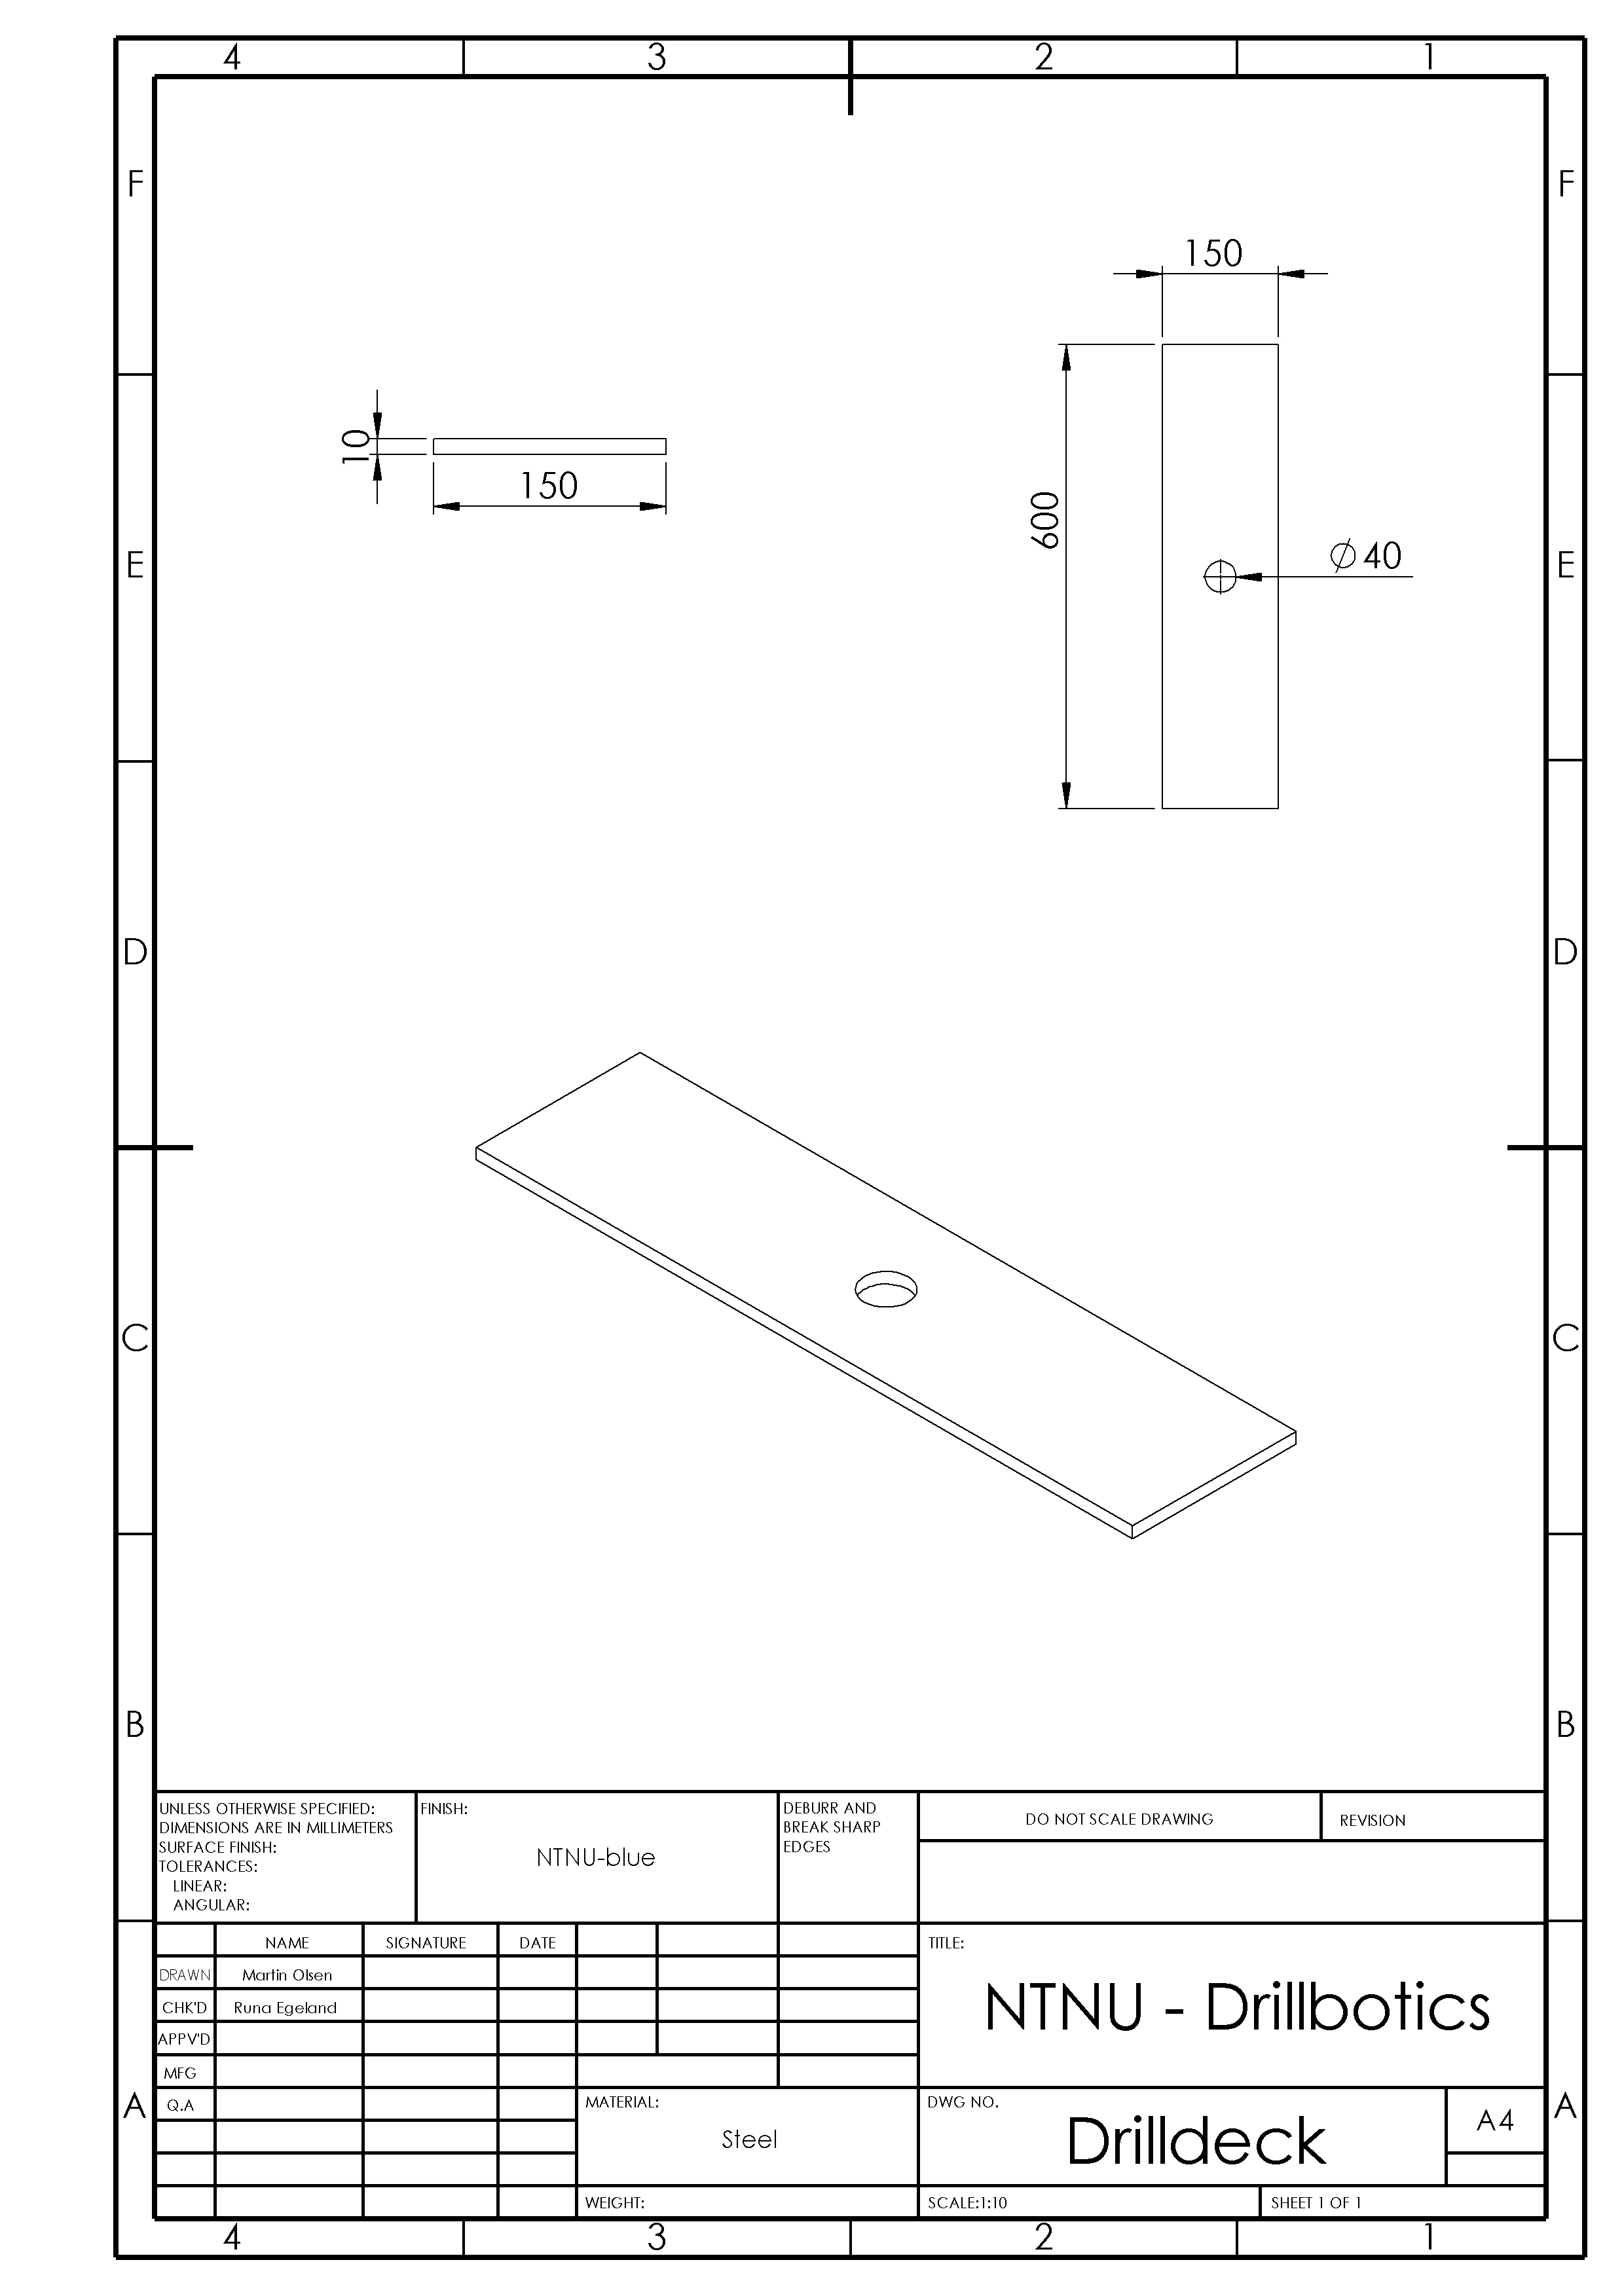
\includegraphics[width=1.0\textwidth]{figures/mechdrawings/Drilldeck.JPG}
\caption{Drilldeck with hole for bushing. All dimensions in mm} 
\label{fig:drilldeck}
\end{figure}

\newpage
\begin{figure} [H]
\centering
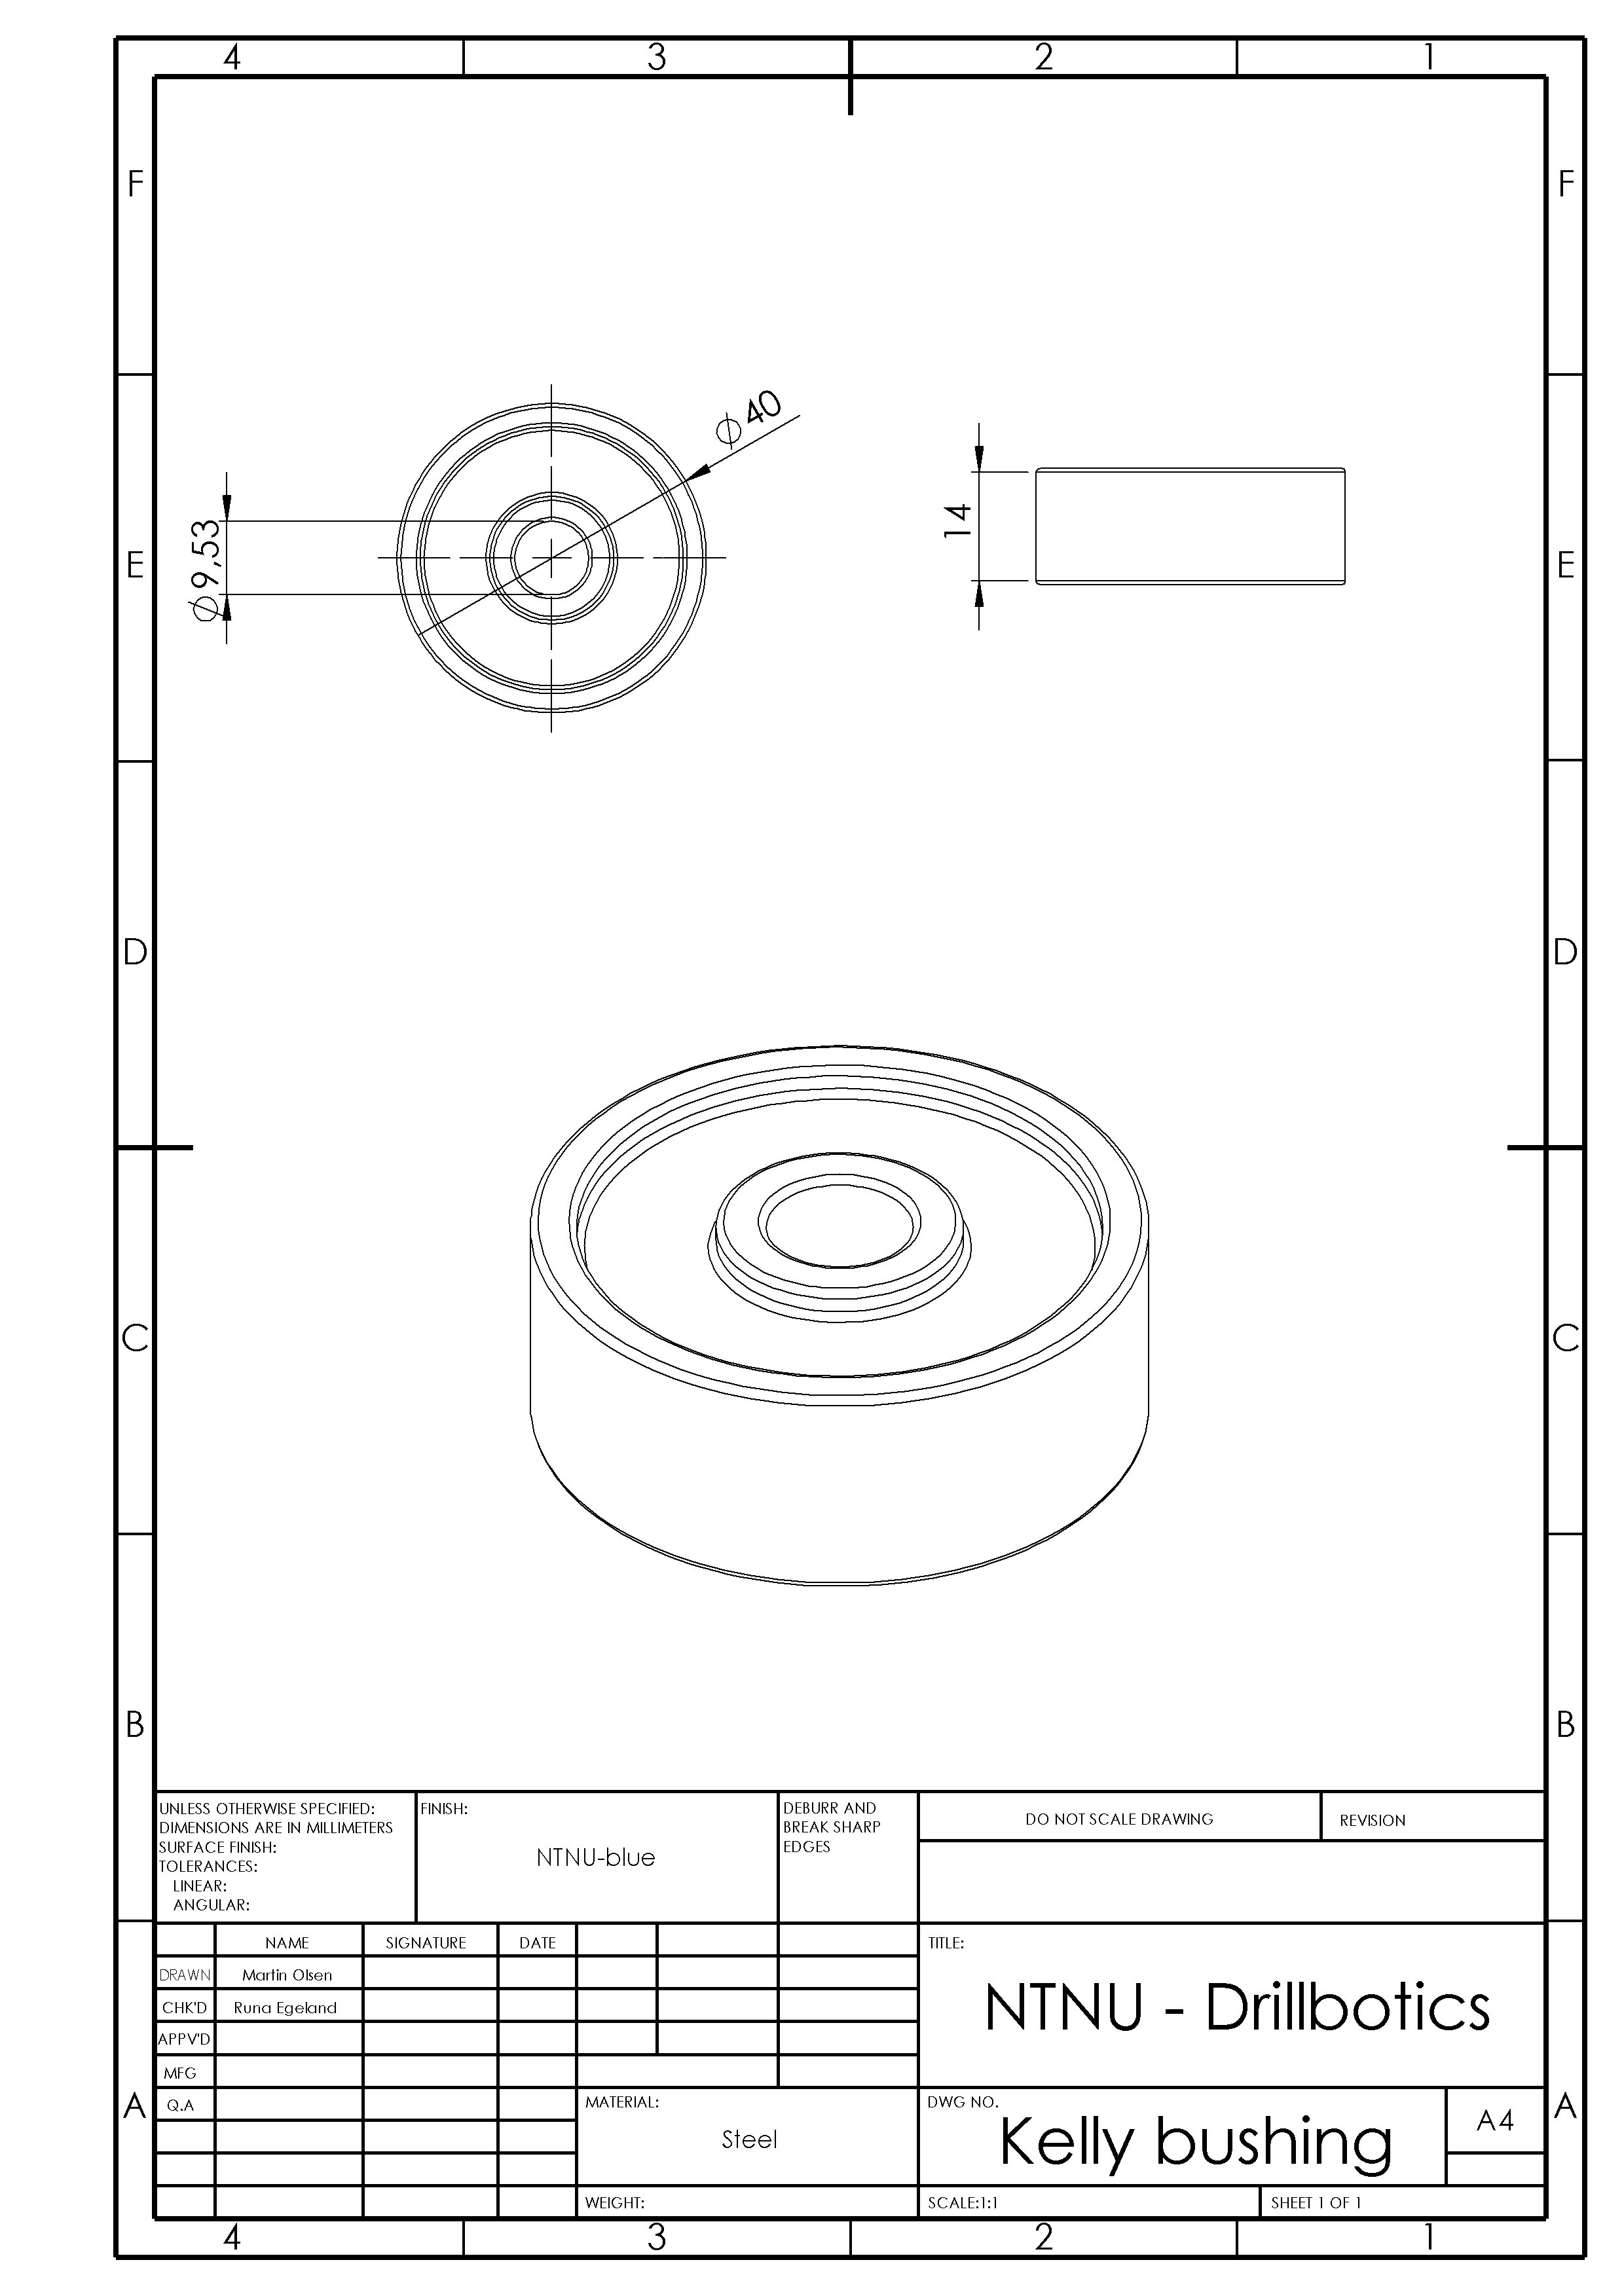
\includegraphics[width=1.0\textwidth]{figures/mechdrawings/Kellybushing.JPG}
\caption{Bushing for drilldeck. All dimensions in mm} 
\label{fig:bushing}
\end{figure}

\newpage
\begin{figure} [H]
\centering
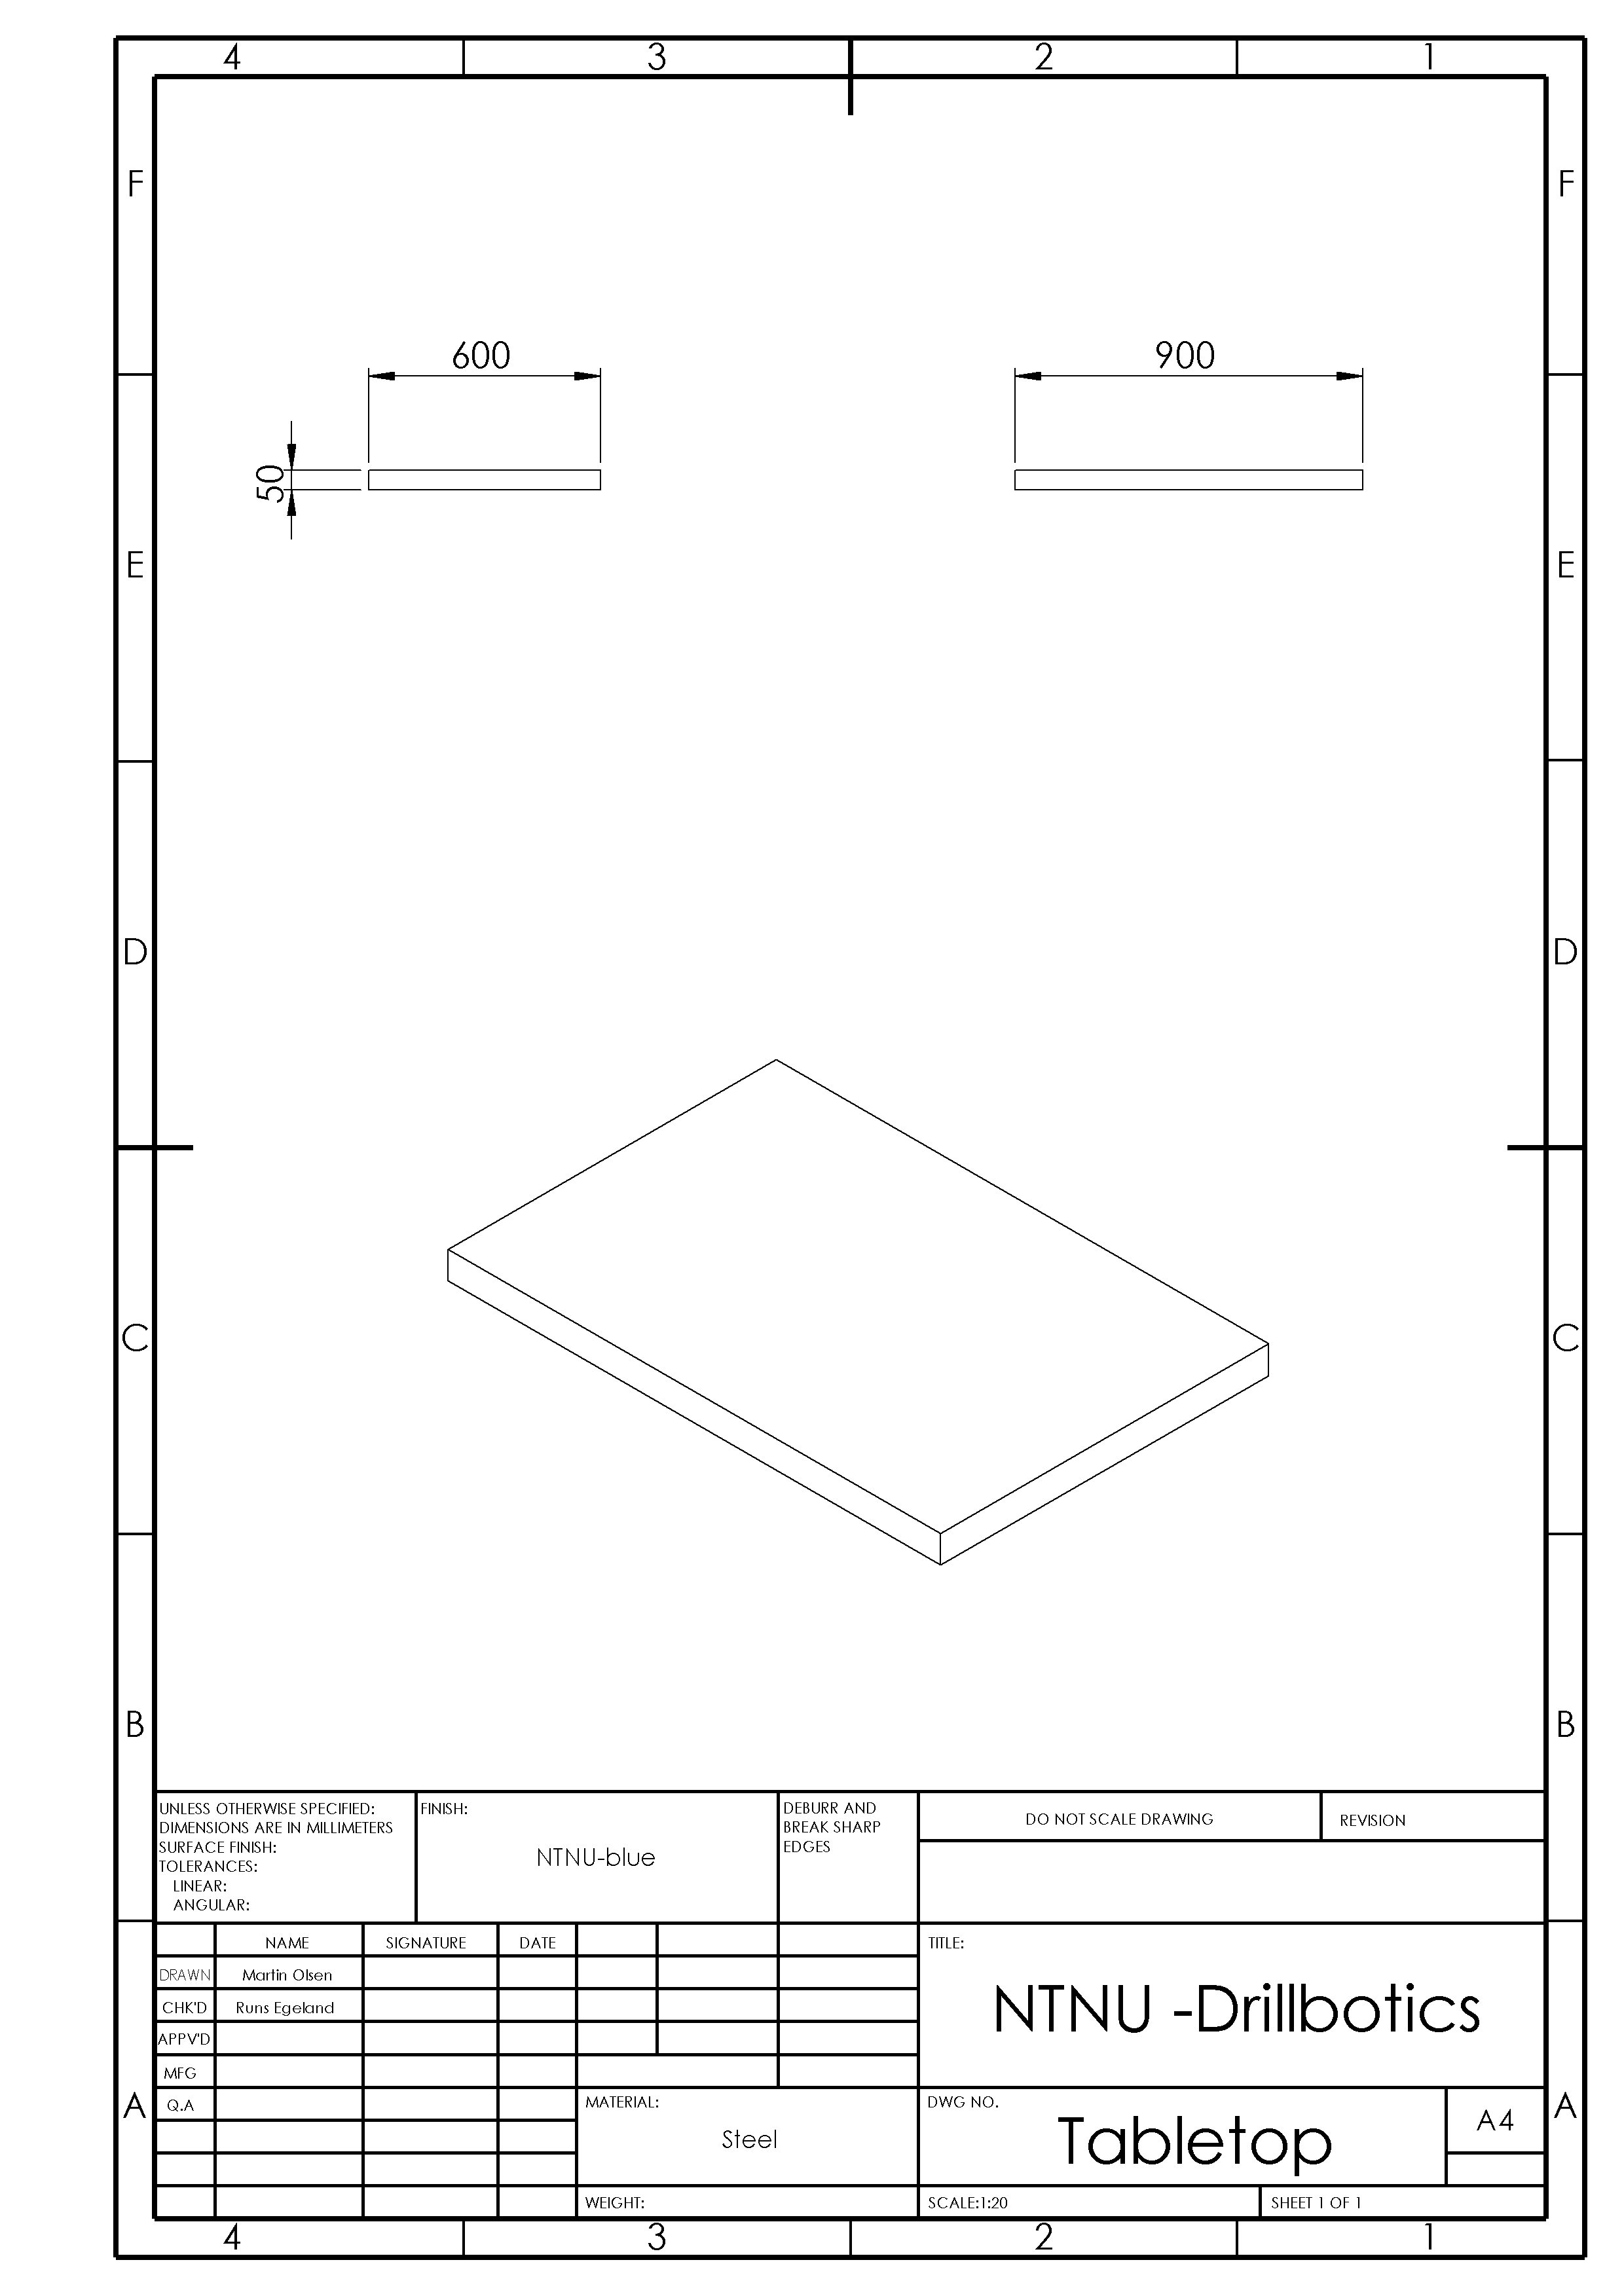
\includegraphics[width=1.0\textwidth]{figures/mechdrawings/Tabletop.JPG}
\caption{Tabletop. All dimensions in mm} 
\label{fig:tabletop}
\end{figure}

\newpage
\begin{figure} [H]
\centering
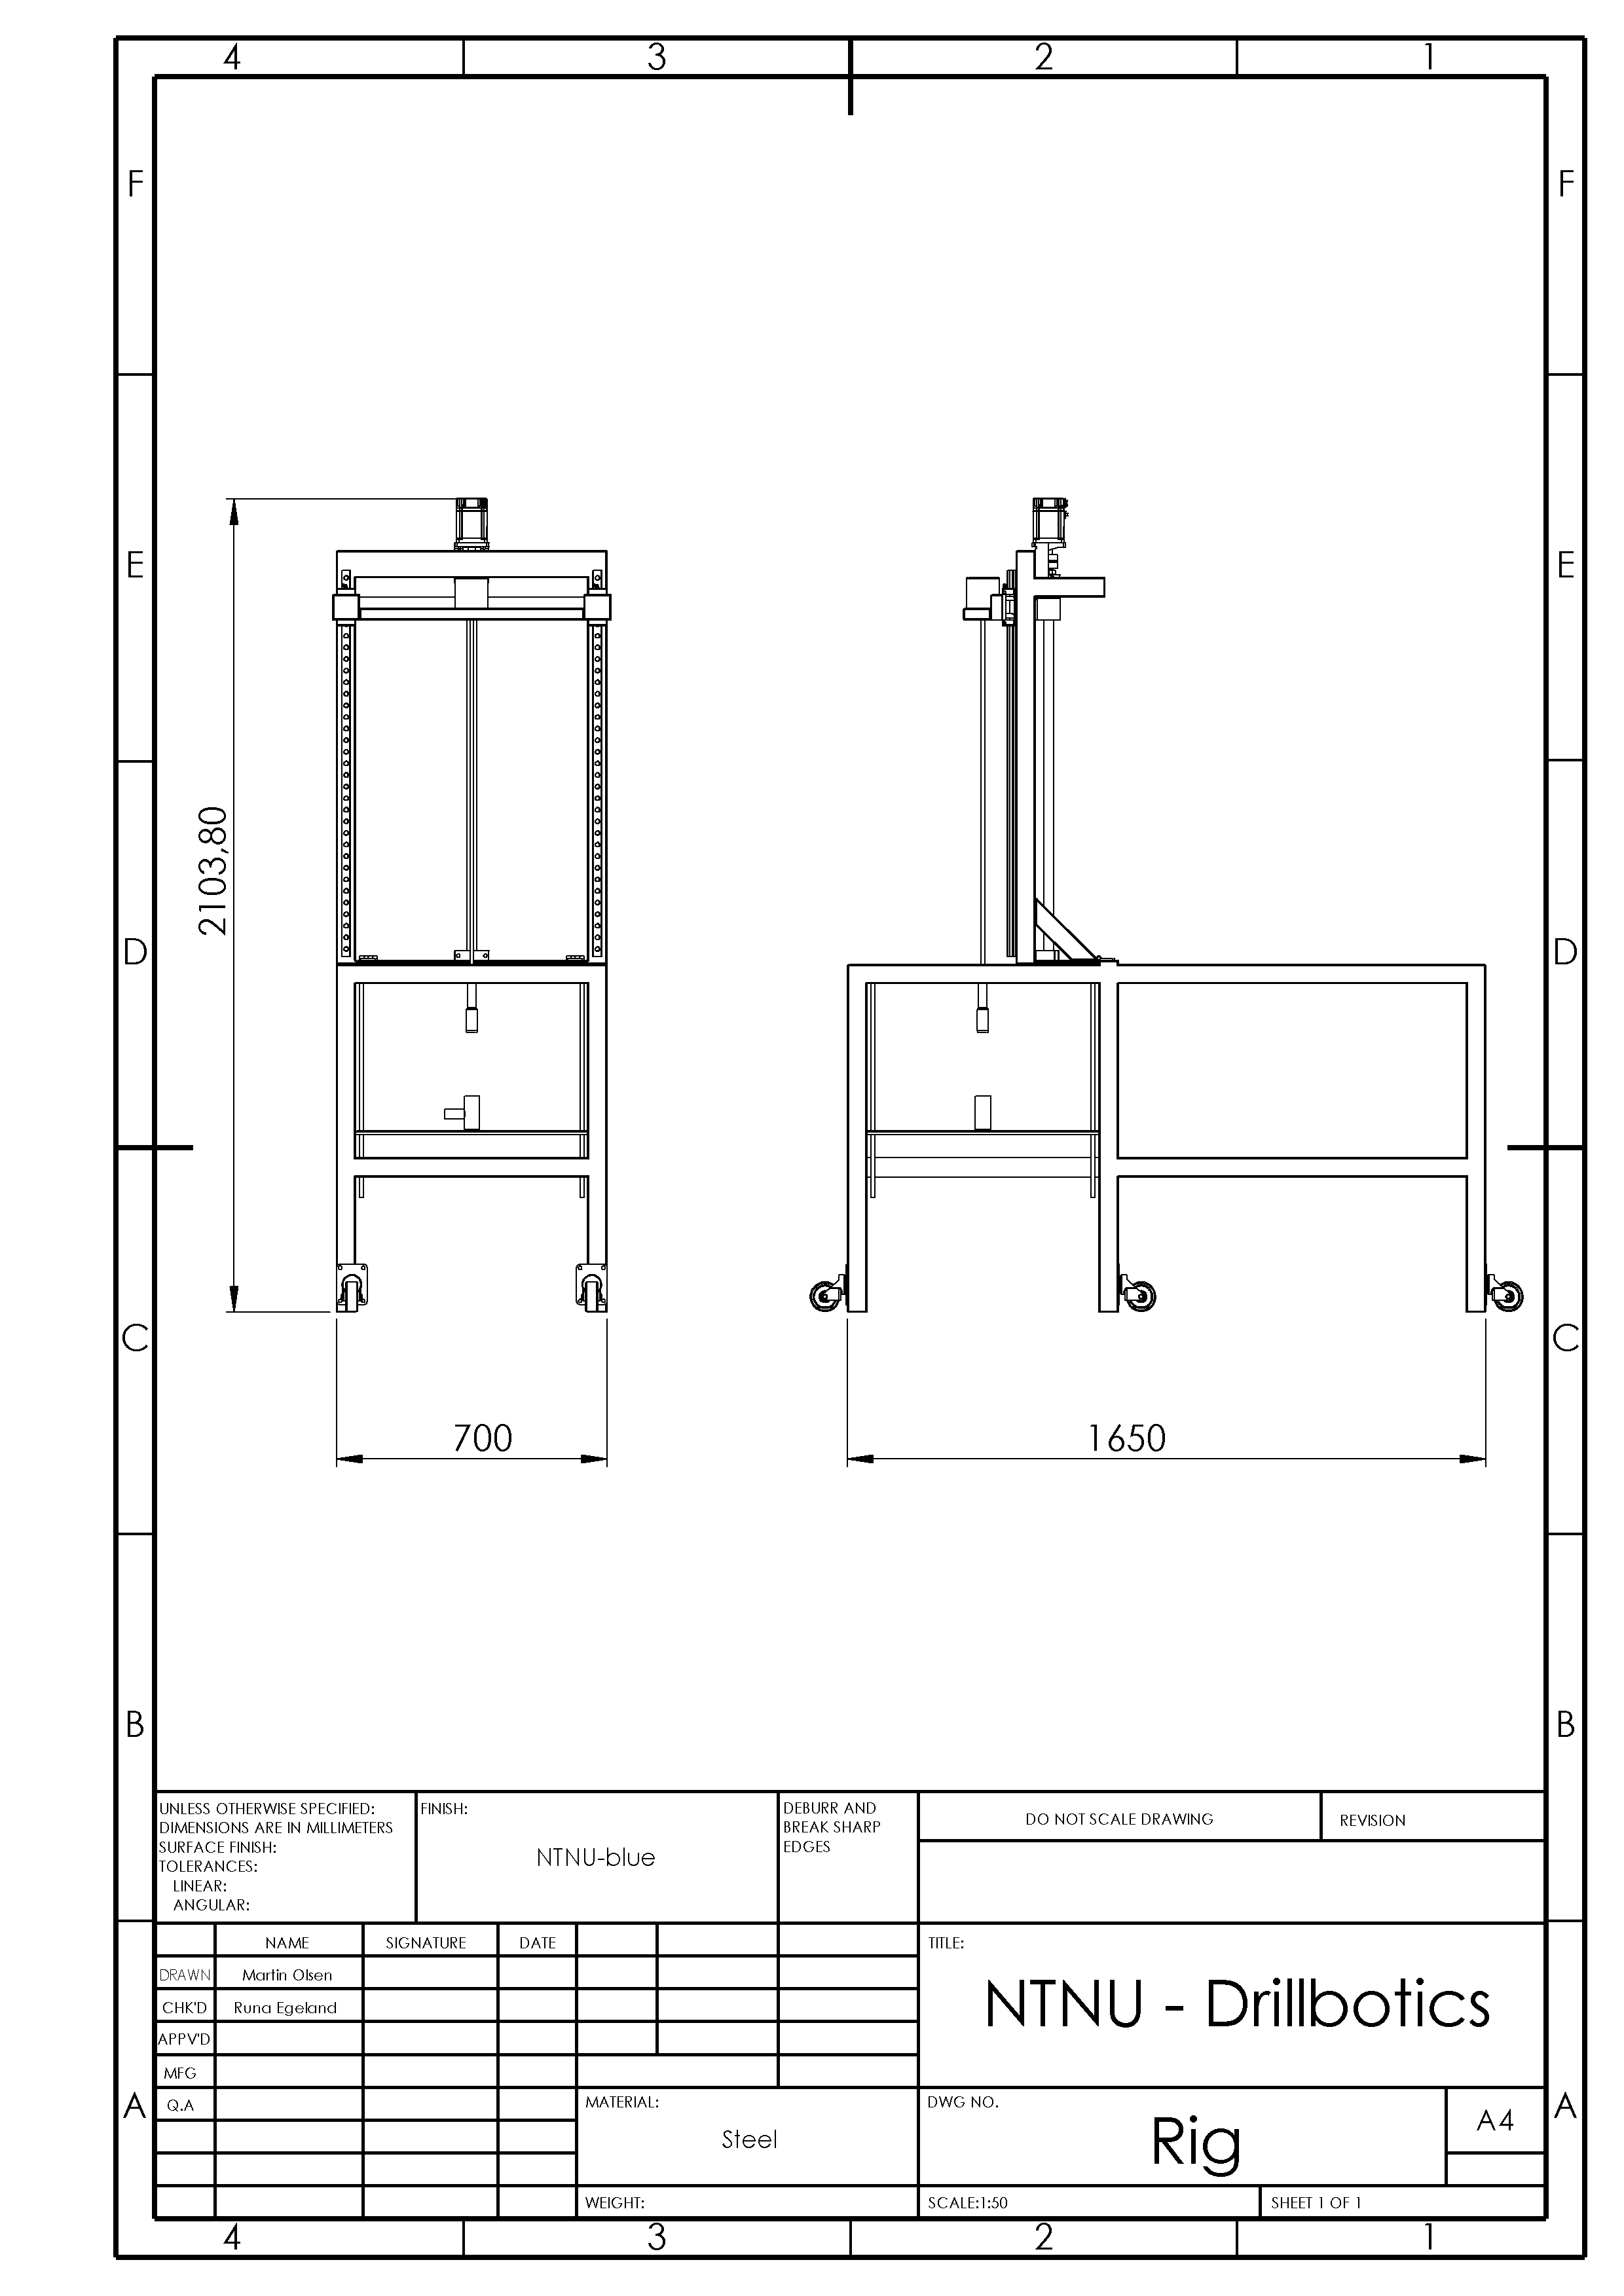
\includegraphics[width=1.0\textwidth]{figures/mechdrawings/Rigfrontandside.JPG}
\caption{Rig viewed from front and side. All dimensions in mm} 
\label{fig:rigview}
\end{figure}

\newpage
\begin{figure} [H]
\centering
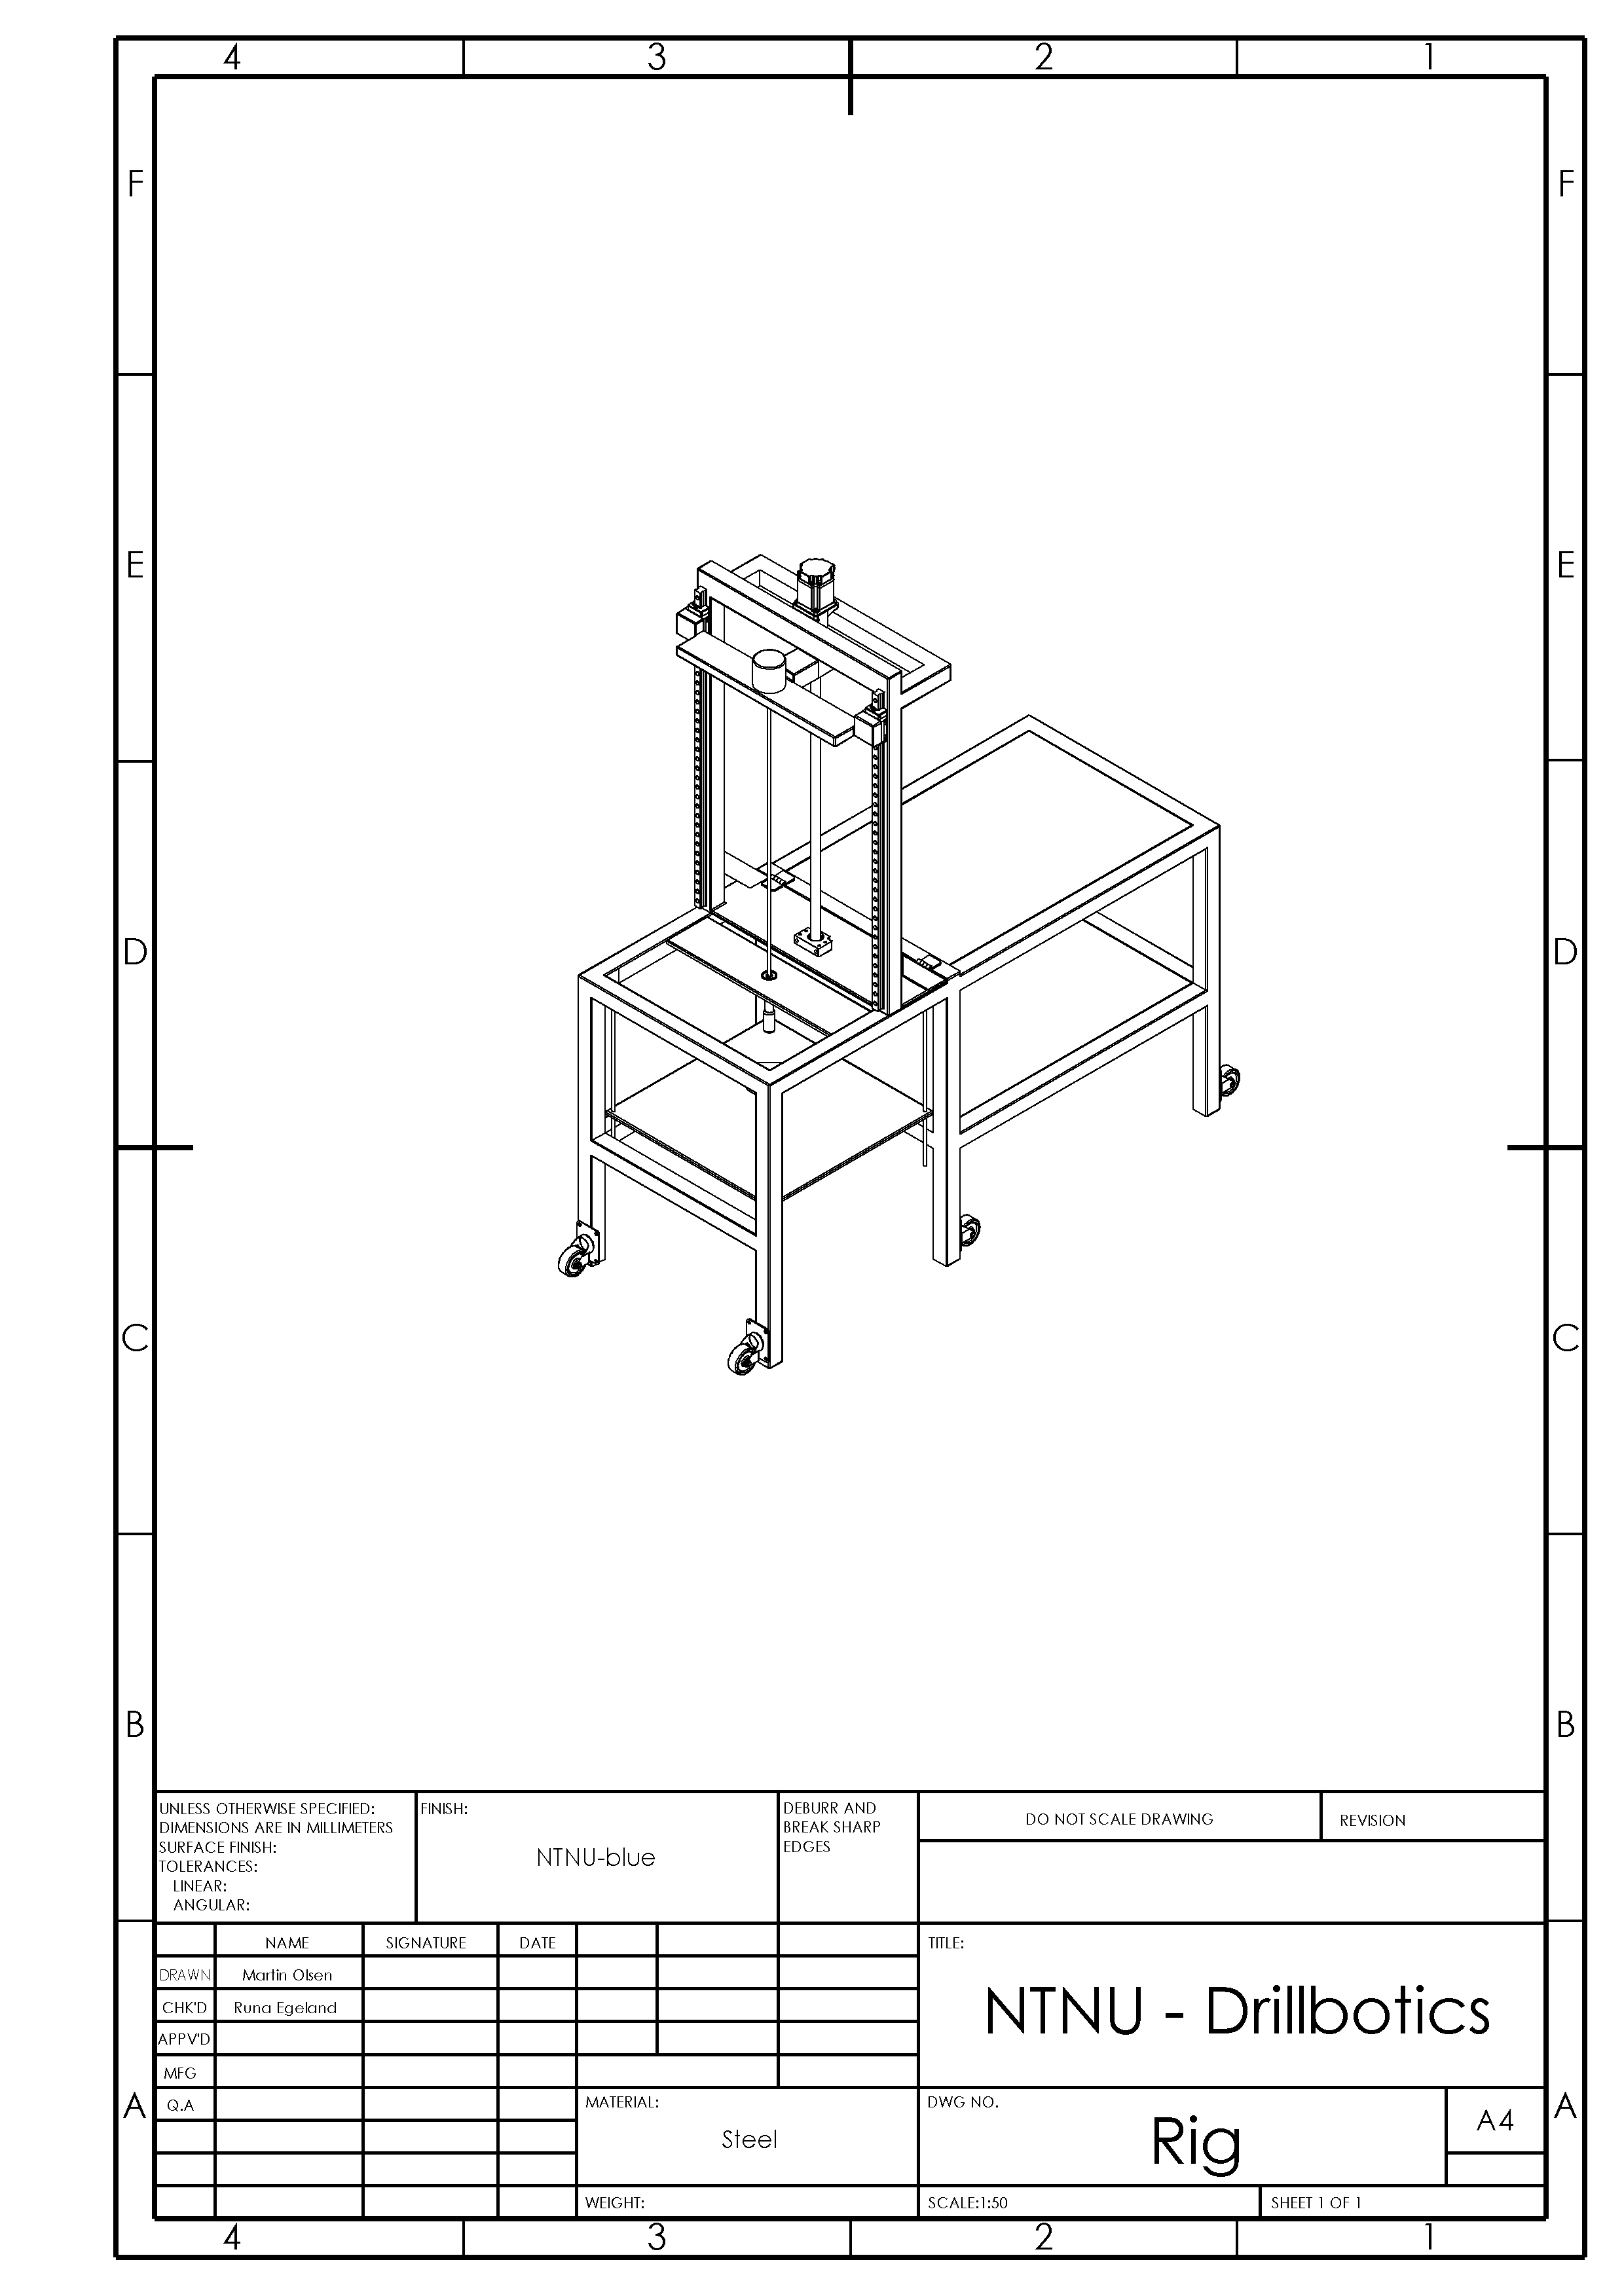
\includegraphics[width=1.0\textwidth]{figures/mechdrawings/Rig.JPG}
\caption{Assembled rig.} 
\label{fig:assemrig}
\end{figure}




\newpage
\section{Title of Appendix B} \label{App:AppendixB}





\end{document}